% Generated by Sphinx.
\def\sphinxdocclass{report}
\documentclass[letterpaper,11pt,english]{sphinxmanual}
\usepackage[utf8]{inputenc}
\DeclareUnicodeCharacter{00A0}{\nobreakspace}
\usepackage[T1]{fontenc}
\usepackage{babel}
\usepackage{times}
\usepackage[Bjarne]{fncychap}
\usepackage{longtable}
\usepackage{sphinx}
\usepackage{multirow}


\title{pypgapack Documentation}
\date{December 17, 2011}
\release{0.1.0}
\author{Jeremy Roberts}
\newcommand{\sphinxlogo}{}
\renewcommand{\releasename}{Release}
\makeindex

\makeatletter
\def\PYG@reset{\let\PYG@it=\relax \let\PYG@bf=\relax%
    \let\PYG@ul=\relax \let\PYG@tc=\relax%
    \let\PYG@bc=\relax \let\PYG@ff=\relax}
\def\PYG@tok#1{\csname PYG@tok@#1\endcsname}
\def\PYG@toks#1+{\ifx\relax#1\empty\else%
    \PYG@tok{#1}\expandafter\PYG@toks\fi}
\def\PYG@do#1{\PYG@bc{\PYG@tc{\PYG@ul{%
    \PYG@it{\PYG@bf{\PYG@ff{#1}}}}}}}
\def\PYG#1#2{\PYG@reset\PYG@toks#1+\relax+\PYG@do{#2}}

\def\PYG@tok@gd{\def\PYG@tc##1{\textcolor[rgb]{0.63,0.00,0.00}{##1}}}
\def\PYG@tok@gu{\let\PYG@bf=\textbf\def\PYG@tc##1{\textcolor[rgb]{0.50,0.00,0.50}{##1}}}
\def\PYG@tok@gt{\def\PYG@tc##1{\textcolor[rgb]{0.00,0.25,0.82}{##1}}}
\def\PYG@tok@gs{\let\PYG@bf=\textbf}
\def\PYG@tok@gr{\def\PYG@tc##1{\textcolor[rgb]{1.00,0.00,0.00}{##1}}}
\def\PYG@tok@cm{\let\PYG@it=\textit\def\PYG@tc##1{\textcolor[rgb]{0.25,0.50,0.56}{##1}}}
\def\PYG@tok@vg{\def\PYG@tc##1{\textcolor[rgb]{0.73,0.38,0.84}{##1}}}
\def\PYG@tok@m{\def\PYG@tc##1{\textcolor[rgb]{0.13,0.50,0.31}{##1}}}
\def\PYG@tok@mh{\def\PYG@tc##1{\textcolor[rgb]{0.13,0.50,0.31}{##1}}}
\def\PYG@tok@cs{\def\PYG@tc##1{\textcolor[rgb]{0.25,0.50,0.56}{##1}}\def\PYG@bc##1{\colorbox[rgb]{1.00,0.94,0.94}{##1}}}
\def\PYG@tok@ge{\let\PYG@it=\textit}
\def\PYG@tok@vc{\def\PYG@tc##1{\textcolor[rgb]{0.73,0.38,0.84}{##1}}}
\def\PYG@tok@il{\def\PYG@tc##1{\textcolor[rgb]{0.13,0.50,0.31}{##1}}}
\def\PYG@tok@go{\def\PYG@tc##1{\textcolor[rgb]{0.19,0.19,0.19}{##1}}}
\def\PYG@tok@cp{\def\PYG@tc##1{\textcolor[rgb]{0.00,0.44,0.13}{##1}}}
\def\PYG@tok@gi{\def\PYG@tc##1{\textcolor[rgb]{0.00,0.63,0.00}{##1}}}
\def\PYG@tok@gh{\let\PYG@bf=\textbf\def\PYG@tc##1{\textcolor[rgb]{0.00,0.00,0.50}{##1}}}
\def\PYG@tok@ni{\let\PYG@bf=\textbf\def\PYG@tc##1{\textcolor[rgb]{0.84,0.33,0.22}{##1}}}
\def\PYG@tok@nl{\let\PYG@bf=\textbf\def\PYG@tc##1{\textcolor[rgb]{0.00,0.13,0.44}{##1}}}
\def\PYG@tok@nn{\let\PYG@bf=\textbf\def\PYG@tc##1{\textcolor[rgb]{0.05,0.52,0.71}{##1}}}
\def\PYG@tok@no{\def\PYG@tc##1{\textcolor[rgb]{0.38,0.68,0.84}{##1}}}
\def\PYG@tok@na{\def\PYG@tc##1{\textcolor[rgb]{0.25,0.44,0.63}{##1}}}
\def\PYG@tok@nb{\def\PYG@tc##1{\textcolor[rgb]{0.00,0.44,0.13}{##1}}}
\def\PYG@tok@nc{\let\PYG@bf=\textbf\def\PYG@tc##1{\textcolor[rgb]{0.05,0.52,0.71}{##1}}}
\def\PYG@tok@nd{\let\PYG@bf=\textbf\def\PYG@tc##1{\textcolor[rgb]{0.33,0.33,0.33}{##1}}}
\def\PYG@tok@ne{\def\PYG@tc##1{\textcolor[rgb]{0.00,0.44,0.13}{##1}}}
\def\PYG@tok@nf{\def\PYG@tc##1{\textcolor[rgb]{0.02,0.16,0.49}{##1}}}
\def\PYG@tok@si{\let\PYG@it=\textit\def\PYG@tc##1{\textcolor[rgb]{0.44,0.63,0.82}{##1}}}
\def\PYG@tok@s2{\def\PYG@tc##1{\textcolor[rgb]{0.25,0.44,0.63}{##1}}}
\def\PYG@tok@vi{\def\PYG@tc##1{\textcolor[rgb]{0.73,0.38,0.84}{##1}}}
\def\PYG@tok@nt{\let\PYG@bf=\textbf\def\PYG@tc##1{\textcolor[rgb]{0.02,0.16,0.45}{##1}}}
\def\PYG@tok@nv{\def\PYG@tc##1{\textcolor[rgb]{0.73,0.38,0.84}{##1}}}
\def\PYG@tok@s1{\def\PYG@tc##1{\textcolor[rgb]{0.25,0.44,0.63}{##1}}}
\def\PYG@tok@gp{\let\PYG@bf=\textbf\def\PYG@tc##1{\textcolor[rgb]{0.78,0.36,0.04}{##1}}}
\def\PYG@tok@sh{\def\PYG@tc##1{\textcolor[rgb]{0.25,0.44,0.63}{##1}}}
\def\PYG@tok@ow{\let\PYG@bf=\textbf\def\PYG@tc##1{\textcolor[rgb]{0.00,0.44,0.13}{##1}}}
\def\PYG@tok@sx{\def\PYG@tc##1{\textcolor[rgb]{0.78,0.36,0.04}{##1}}}
\def\PYG@tok@bp{\def\PYG@tc##1{\textcolor[rgb]{0.00,0.44,0.13}{##1}}}
\def\PYG@tok@c1{\let\PYG@it=\textit\def\PYG@tc##1{\textcolor[rgb]{0.25,0.50,0.56}{##1}}}
\def\PYG@tok@kc{\let\PYG@bf=\textbf\def\PYG@tc##1{\textcolor[rgb]{0.00,0.44,0.13}{##1}}}
\def\PYG@tok@c{\let\PYG@it=\textit\def\PYG@tc##1{\textcolor[rgb]{0.25,0.50,0.56}{##1}}}
\def\PYG@tok@mf{\def\PYG@tc##1{\textcolor[rgb]{0.13,0.50,0.31}{##1}}}
\def\PYG@tok@err{\def\PYG@bc##1{\fcolorbox[rgb]{1.00,0.00,0.00}{1,1,1}{##1}}}
\def\PYG@tok@kd{\let\PYG@bf=\textbf\def\PYG@tc##1{\textcolor[rgb]{0.00,0.44,0.13}{##1}}}
\def\PYG@tok@ss{\def\PYG@tc##1{\textcolor[rgb]{0.32,0.47,0.09}{##1}}}
\def\PYG@tok@sr{\def\PYG@tc##1{\textcolor[rgb]{0.14,0.33,0.53}{##1}}}
\def\PYG@tok@mo{\def\PYG@tc##1{\textcolor[rgb]{0.13,0.50,0.31}{##1}}}
\def\PYG@tok@mi{\def\PYG@tc##1{\textcolor[rgb]{0.13,0.50,0.31}{##1}}}
\def\PYG@tok@kn{\let\PYG@bf=\textbf\def\PYG@tc##1{\textcolor[rgb]{0.00,0.44,0.13}{##1}}}
\def\PYG@tok@o{\def\PYG@tc##1{\textcolor[rgb]{0.40,0.40,0.40}{##1}}}
\def\PYG@tok@kr{\let\PYG@bf=\textbf\def\PYG@tc##1{\textcolor[rgb]{0.00,0.44,0.13}{##1}}}
\def\PYG@tok@s{\def\PYG@tc##1{\textcolor[rgb]{0.25,0.44,0.63}{##1}}}
\def\PYG@tok@kp{\def\PYG@tc##1{\textcolor[rgb]{0.00,0.44,0.13}{##1}}}
\def\PYG@tok@w{\def\PYG@tc##1{\textcolor[rgb]{0.73,0.73,0.73}{##1}}}
\def\PYG@tok@kt{\def\PYG@tc##1{\textcolor[rgb]{0.56,0.13,0.00}{##1}}}
\def\PYG@tok@sc{\def\PYG@tc##1{\textcolor[rgb]{0.25,0.44,0.63}{##1}}}
\def\PYG@tok@sb{\def\PYG@tc##1{\textcolor[rgb]{0.25,0.44,0.63}{##1}}}
\def\PYG@tok@k{\let\PYG@bf=\textbf\def\PYG@tc##1{\textcolor[rgb]{0.00,0.44,0.13}{##1}}}
\def\PYG@tok@se{\let\PYG@bf=\textbf\def\PYG@tc##1{\textcolor[rgb]{0.25,0.44,0.63}{##1}}}
\def\PYG@tok@sd{\let\PYG@it=\textit\def\PYG@tc##1{\textcolor[rgb]{0.25,0.44,0.63}{##1}}}

\def\PYGZbs{\char`\\}
\def\PYGZus{\char`\_}
\def\PYGZob{\char`\{}
\def\PYGZcb{\char`\}}
\def\PYGZca{\char`\^}
\def\PYGZsh{\char`\#}
\def\PYGZpc{\char`\%}
\def\PYGZdl{\char`\$}
\def\PYGZti{\char`\~}
% for compatibility with earlier versions
\def\PYGZat{@}
\def\PYGZlb{[}
\def\PYGZrb{]}
\makeatother

\begin{document}

\maketitle
\tableofcontents
\phantomsection\label{index::doc}



\chapter{Getting Started With pypgapack}
\label{getting_started::doc}\label{getting_started:getting-started-with-pypgapack}\label{getting_started:pypgapack-a-light-python-wrapper-for-pgapack}\label{getting_started:sec-getting-started}

\section{Background}
\label{getting_started:background}
\code{pypgapack} is a Python wrapper for the parallel genetic
algorithm library pgapack, written in C by David Levine.
The source and documentation for pgapack can be found at
\href{http://ftp.mcs.anl.gov/pub/pgapack/}{http://ftp.mcs.anl.gov/pub/pgapack/}.
The motivation for wrapping the code is ultimately to support
a class project aiming to optimize loading patterns of
nuclear reactor cores, which is a rather large and difficult
combinatorial problem.  Lots of researchers have applied genetic algorithms
(and many other algorithms) to the problem, and the class project
aims to provide a flexible test bench in Python to investigate
various ideas.  Wrapping pgapack is one step toward that goal.
pgapAck was chose largely due to limited but positive past
experience with it.

It should be pointed out that a similar effort to wrap pgapack
in Python was made called \code{pgapy} (see \href{http://pgapy.sourceforge.net/}{http://pgapy.sourceforge.net/}), but I actually couldn't get it
to work, probably because I didn't know a thing about building
Python modules before I started this (and my minimal C knowledge
didn't help matters).  Hence, I decided to ``roll my own'' using
\href{http://www.swig.org/}{SWIG} in combination with a C++ wrapper
around pgapack instead of interfacing directly with pgapack
as \code{pgapy} does.

The {\hyperref[api_reference:PGA]{\code{PGA}}} class wraps almost all of pgapack's functionality,
including allowing user functions for several operations (like
initialization, crossover, etc.) for the \code{PGA.DATATYPE\_BINARY},
\code{PGA.DATATYPE\_REAL} and \code{PGA.DATATYPE\_INTEGER} alleles.
No such support is currently offered for other allele types,
including user-specified types.  The intended way to use
\code{pypgapack} is to derive classes from {\hyperref[api_reference:PGA]{\code{PGA}}}, with
objective and other functions as members.

Parallel functionality is supported with the help of
\href{http://mpi4py.scipy.org/}{mpi4py}.

\begin{notice}{note}{Note:}
\code{pypgapack} is currently in beta mode, so there may be many
things that look wrapped but are not.  Testing is a future goal,
but not a priority---I need a grade!  Feedback is welcome at
\href{mailto:robertsj@mit.edu}{robertsj@mit.edu}.
\end{notice}


\section{Building pypgapack}
\label{getting_started:building-pypgapack}
Included in ./pypgapack are the required source files and a simple script
\code{build\_pypgapack} which generates the Python module.  To build, do
the following:
\begin{enumerate}
\item {} 
Build PGAPack with the patches in ./patches.  The major difference is
a slight change to allow use with C++.  The Makefile template also is
set to produce shared and static libraries.

\item {} 
Modify the paths and variables in \code{build\_pypgapack} below to suit
your needs.

\item {} 
The source as distributed is set for serial.  To use in parallel, do
the following:
\begin{itemize}
\item {} 
Uncomment \code{PARALLEL} in \code{build\_pypgapack}

\item {} 
Set \code{CXX} to the appropriate compiler (e.g. mpic++)
in \code{build\_pypgapack}

\item {} 
Delete or move the dummy \code{mpi.h} included with PGAPack to avoid
redefinitions.  There's probably a better approach.

\item {} 
This assumes PGAPack was built in parallel; if not, do so.  Refer to
the PGAPack documentation.  You need an MPI-enabled compiler.

\item {} 
Get mpi4py (e.g. easy\_install mpi4py). You need an MPI-enabled compiler.
Note, a few files from mpi4py are included in ./pypgapack/mpi4py.  These
\emph{may} need to be updated.

\end{itemize}

\item {} 
Execute \code{build\_pypgapack} and set PYTHONPATH accordingly.

\end{enumerate}


\section{Next Steps}
\label{getting_started:next-steps}
The user is encouraged to read the pgapack documentation thoroughly
before using pypgapack, as the shared API is \emph{not} covered in this
documentation (and neither are the many PGAPack defaults).  It's
helpful to go through their examples in C/C++ or Fortran if you
know the languages.

Thereafter, see the collection of {\hyperref[examples:sec-examples]{\emph{Examples}}}, which
include several of the original pgapack examples along with a few additional
ones that demonstrate how to use user-defined functions for a variety
of operations.  Reference output is included, though don't expect
to reproduce the numbers exactly for the small number of generations
used, as they'll be sensitive to compilation, etc.

For a quick refresher, the basic gist of genetic algorithms is
discussed briefly
in {\hyperref[methods:sec-methods]{\emph{Methods}}}, which lists a few references that may
be of use.

Documentation for the relatively small number of additional methods
not explicitly in pgapack can be found in the {\hyperref[api_reference:sec-reference]{\emph{API Reference}}}.


\chapter{Examples}
\label{examples:sec-examples}\label{examples::doc}\label{examples:examples}
All examples are located in the \code{pypgapack/examples} and the
reference output for all examples is in \code{pypgapack/examples/output}.
Aside from small floating point differences, the values should be
the same given the use of a fixed random number generator seed in
all the examples.  A utility script \code{run\_examples.py} is included
to test user output to the included reference cases.  (Note, the above
might actually be untrue, as compilation can and will change how
a fixed pseudo-random number sequence is generated.)

Also, the maximum generation count is limited to
50 for all cases to produce short output.  Experiment with that limit
to see better solutions.


\section{Basic Examples}
\label{examples:basic-examples}\label{examples:sec-basicexamples}
The following are some simple examples that illustrate
the basic PGAPack functionality.


\subsection{Example 1: MAXBIT}
\label{examples:example-1-maxbit}\label{examples:sec-maxbitexample}
\code{pypgapack} is pretty easy to use, and to demonstrate, we'll solve
the maxbit problem, the first example in the PGAPack documentation.

\begin{Verbatim}[commandchars=\\\{\},numbers=left,firstnumber=1,stepnumber=1]
\PYG{l+s+sd}{"""}
\PYG{l+s+sd}{pypgapack/examples/example01.py  --  maxbit}
\PYG{l+s+sd}{"""}
\PYG{k+kn}{from} \PYG{n+nn}{pypgapack} \PYG{k+kn}{import} \PYG{n}{PGA}
\PYG{k+kn}{import} \PYG{n+nn}{sys}
\PYG{k}{class} \PYG{n+nc}{MyPGA}\PYG{p}{(}\PYG{n}{PGA}\PYG{p}{)} \PYG{p}{:}
    \PYG{l+s+sd}{"""  }
\PYG{l+s+sd}{    Derive our own class from PGA.}
\PYG{l+s+sd}{    """}
    \PYG{k}{def} \PYG{n+nf}{maxbit}\PYG{p}{(}\PYG{n+nb+bp}{self}\PYG{p}{,} \PYG{n}{p}\PYG{p}{,} \PYG{n}{pop}\PYG{p}{)} \PYG{p}{:}
        \PYG{l+s+sd}{"""}
\PYG{l+s+sd}{        Maximum when all alleles are 1's, and that maximum is n. }
\PYG{l+s+sd}{        """}
        \PYG{n}{val} \PYG{o}{=} \PYG{l+m+mi}{0}
        \PYG{c}{\PYGZsh{} Size of the problem}
        \PYG{n}{n} \PYG{o}{=} \PYG{n+nb+bp}{self}\PYG{o}{.}\PYG{n}{GetStringLength}\PYG{p}{(}\PYG{p}{)}               
        \PYG{k}{for} \PYG{n}{i} \PYG{o+ow}{in} \PYG{n+nb}{range}\PYG{p}{(}\PYG{l+m+mi}{0}\PYG{p}{,} \PYG{n}{n}\PYG{p}{)} \PYG{p}{:}               
            \PYG{c}{\PYGZsh{} Check whether ith allele in string p is 1}
            \PYG{k}{if} \PYG{n+nb+bp}{self}\PYG{o}{.}\PYG{n}{GetBinaryAllele}\PYG{p}{(}\PYG{n}{p}\PYG{p}{,} \PYG{n}{pop}\PYG{p}{,} \PYG{n}{i}\PYG{p}{)} \PYG{p}{:} 
                \PYG{n}{val} \PYG{o}{=} \PYG{n}{val} \PYG{o}{+} \PYG{l+m+mi}{1}
        \PYG{c}{\PYGZsh{} Remember that fitness evaluations must return a float}
        \PYG{k}{return} \PYG{n+nb}{float}\PYG{p}{(}\PYG{n}{val}\PYG{p}{)}      
                
\PYG{c}{\PYGZsh{} (Command line arguments, 1's and 0's, string length, and maximize it)}
\PYG{n}{opt} \PYG{o}{=} \PYG{n}{MyPGA}\PYG{p}{(}\PYG{n}{sys}\PYG{o}{.}\PYG{n}{argv}\PYG{p}{,} \PYG{n}{PGA}\PYG{o}{.}\PYG{n}{DATATYPE\PYGZus{}BINARY}\PYG{p}{,} \PYG{l+m+mi}{100}\PYG{p}{,} \PYG{n}{PGA}\PYG{o}{.}\PYG{n}{MAXIMIZE}\PYG{p}{)}
\PYG{n}{opt}\PYG{o}{.}\PYG{n}{SetRandomSeed}\PYG{p}{(}\PYG{l+m+mi}{1}\PYG{p}{)}       \PYG{c}{\PYGZsh{} Set random seed for verification.}
\PYG{n}{opt}\PYG{o}{.}\PYG{n}{SetMaxGAIterValue}\PYG{p}{(}\PYG{l+m+mi}{50}\PYG{p}{)}  \PYG{c}{\PYGZsh{} 50 generations (default 1000) for short output.}
\PYG{n}{opt}\PYG{o}{.}\PYG{n}{SetUp}\PYG{p}{(}\PYG{p}{)}                \PYG{c}{\PYGZsh{} Internal allocations, etc.}
\PYG{n}{opt}\PYG{o}{.}\PYG{n}{Run}\PYG{p}{(}\PYG{n}{opt}\PYG{o}{.}\PYG{n}{maxbit}\PYG{p}{)}        \PYG{c}{\PYGZsh{} Set the objective.}
\PYG{n}{opt}\PYG{o}{.}\PYG{n}{Destroy}\PYG{p}{(}\PYG{p}{)}              \PYG{c}{\PYGZsh{} Clean up PGAPack internals}
\end{Verbatim}

Running it yields the following output:

\begin{Verbatim}[commandchars=\\\{\}]
***Constructing PGA***
Iter \#     Field      Value
10         Best       6.900000e+01
Iter \#     Field      Value
20         Best       7.200000e+01
Iter \#     Field      Value
30         Best       7.600000e+01
Iter \#     Field      Value
40         Best       7.700000e+01
Iter \#     Field      Value
50         Best       8.000000e+01
The Best Evaluation: 8.000000e+01.
The Best String:
[ 0111110111101111011111100111011110111101111111011111110100111111 ]
[ 011111110111110111111110111101011011 ]
***Destroying PGA context***
\end{Verbatim}


\subsection{Example 2: MAXINT}
\label{examples:example-2-maxint}\label{examples:sec-maxintexample}
This is a similar problem, but the alleles are integers ranging
from -100 to 100.  Note that when the integer ranges are
set, a cast to \code{intc} is used.  Python uses high precision
datatypes, and there doesn't seem to be a safe implicit conversion
between the Python integer type and the C integer type behind
the scenes (in SWIG land).  Casting
explicitly circumvents the issue.

\begin{Verbatim}[commandchars=\\\{\},numbers=left,firstnumber=1,stepnumber=1]
\PYG{l+s+sd}{"""}
\PYG{l+s+sd}{pypgapack/examples/example02.py  --  maxint}
\PYG{l+s+sd}{"""}
\PYG{k+kn}{from} \PYG{n+nn}{pypgapack} \PYG{k+kn}{import} \PYG{n}{PGA}
\PYG{k+kn}{import} \PYG{n+nn}{numpy} \PYG{k+kn}{as} \PYG{n+nn}{np}
\PYG{k+kn}{import} \PYG{n+nn}{sys}
\PYG{k}{class} \PYG{n+nc}{MyPGA}\PYG{p}{(}\PYG{n}{PGA}\PYG{p}{)} \PYG{p}{:}
    \PYG{l+s+sd}{"""  }
\PYG{l+s+sd}{    Derive our own class from PGA.}
\PYG{l+s+sd}{    """}
    \PYG{k}{def} \PYG{n+nf}{maxint}\PYG{p}{(}\PYG{n+nb+bp}{self}\PYG{p}{,} \PYG{n}{p}\PYG{p}{,} \PYG{n}{pop}\PYG{p}{)} \PYG{p}{:}
        \PYG{l+s+sd}{"""}
\PYG{l+s+sd}{        The maximum integer sum problem.}
\PYG{l+s+sd}{    }
\PYG{l+s+sd}{        The alleles are integers, and we solve}
\PYG{l+s+sd}{            max f(x) = x\PYGZus{}1 + x\PYGZus{}2 + ... + x\PYGZus{}N}
\PYG{l+s+sd}{        subject to}
\PYG{l+s+sd}{            \textbar{}x\PYGZus{}i\textbar{} \textless{}= 100 .}
\PYG{l+s+sd}{        That maximum is f(x) = 100n obtained for x\PYGZus{}i = 100 for all i.}
\PYG{l+s+sd}{        """}
        \PYG{n}{c} \PYG{o}{=} \PYG{n+nb+bp}{self}\PYG{o}{.}\PYG{n}{GetIntegerChromosome}\PYG{p}{(}\PYG{n}{p}\PYG{p}{,} \PYG{n}{pop}\PYG{p}{)} \PYG{c}{\PYGZsh{} Get pth string as Numpy array }
        \PYG{n}{val} \PYG{o}{=} \PYG{n}{np}\PYG{o}{.}\PYG{n}{sum}\PYG{p}{(}\PYG{n}{c}\PYG{p}{)}                       \PYG{c}{\PYGZsh{}   and sum it up.     }
        \PYG{k}{del} \PYG{n}{c}                                 \PYG{c}{\PYGZsh{} Delete "view" to internals.}
        \PYG{k}{return} \PYG{n+nb}{float}\PYG{p}{(}\PYG{n}{val}\PYG{p}{)}                     \PYG{c}{\PYGZsh{} Always return a float.   }
        
\PYG{n}{n}   \PYG{o}{=} \PYG{l+m+mi}{10}                \PYG{c}{\PYGZsh{} String length.}
\PYG{c}{\PYGZsh{} (Command line arguments, integers, string length, and maximize it)}
\PYG{n}{opt} \PYG{o}{=} \PYG{n}{MyPGA}\PYG{p}{(}\PYG{n}{sys}\PYG{o}{.}\PYG{n}{argv}\PYG{p}{,} \PYG{n}{PGA}\PYG{o}{.}\PYG{n}{DATATYPE\PYGZus{}INTEGER}\PYG{p}{,} \PYG{n}{n}\PYG{p}{,} \PYG{n}{PGA}\PYG{o}{.}\PYG{n}{MAXIMIZE}\PYG{p}{)}
\PYG{n}{opt}\PYG{o}{.}\PYG{n}{SetRandomSeed}\PYG{p}{(}\PYG{l+m+mi}{1}\PYG{p}{)}    \PYG{c}{\PYGZsh{} Set random seed for verification.}
\PYG{n}{u\PYGZus{}b} \PYG{o}{=}  \PYG{l+m+mi}{100}\PYG{o}{*}\PYG{n}{np}\PYG{o}{.}\PYG{n}{ones}\PYG{p}{(}\PYG{n}{n}\PYG{p}{)}   \PYG{c}{\PYGZsh{} Define lower bound.}
\PYG{n}{l\PYGZus{}b} \PYG{o}{=} \PYG{o}{-}\PYG{l+m+mi}{100}\PYG{o}{*}\PYG{n}{np}\PYG{o}{.}\PYG{n}{ones}\PYG{p}{(}\PYG{n}{n}\PYG{p}{)}   \PYG{c}{\PYGZsh{} Define upper bound.}
\PYG{c}{\PYGZsh{} Set the bounds.  Note, need to cast as C-combatible integers.}
\PYG{n}{opt}\PYG{o}{.}\PYG{n}{SetIntegerInitRange}\PYG{p}{(}\PYG{n}{l\PYGZus{}b}\PYG{o}{.}\PYG{n}{astype}\PYG{p}{(}\PYG{l+s}{'}\PYG{l+s}{intc}\PYG{l+s}{'}\PYG{p}{)}\PYG{p}{,} \PYG{n}{u\PYGZus{}b}\PYG{o}{.}\PYG{n}{astype}\PYG{p}{(}\PYG{l+s}{'}\PYG{l+s}{intc}\PYG{l+s}{'}\PYG{p}{)}\PYG{p}{)} 
\PYG{n}{opt}\PYG{o}{.}\PYG{n}{SetMaxGAIterValue}\PYG{p}{(}\PYG{l+m+mi}{50}\PYG{p}{)}    \PYG{c}{\PYGZsh{} 50 generations for short output.}
\PYG{n}{opt}\PYG{o}{.}\PYG{n}{SetUp}\PYG{p}{(}\PYG{p}{)}                  \PYG{c}{\PYGZsh{} Internal allocations, etc.}
\PYG{n}{opt}\PYG{o}{.}\PYG{n}{Run}\PYG{p}{(}\PYG{n}{opt}\PYG{o}{.}\PYG{n}{maxint}\PYG{p}{)}          \PYG{c}{\PYGZsh{} Set the objective.}
\PYG{n}{opt}\PYG{o}{.}\PYG{n}{Destroy}\PYG{p}{(}\PYG{p}{)}                \PYG{c}{\PYGZsh{} Clean up PGAPack internals.}
\end{Verbatim}

Running it yields the following output:

\begin{Verbatim}[commandchars=\\\{\}]
***Constructing PGA***
Iter \#     Field      Value
10         Best       5.100000e+02
Iter \#     Field      Value
20         Best       6.480000e+02
Iter \#     Field      Value
30         Best       7.150000e+02
Iter \#     Field      Value
40         Best       7.760000e+02
Iter \#     Field      Value
50         Best       8.220000e+02
The Best Evaluation: 8.220000e+02.
The Best String:
\#    0: [      27], [     100], [      86], [      98], [      97], [      99]
\#    6: [      79], [      89], [      64], [      83]

***Destroying PGA context***
\end{Verbatim}


\subsection{Example 3: MAXREAL}
\label{examples:sec-maxrealexample}\label{examples:example-3-maxreal}
This is the same problem, but for real alleles.  Here, note use
of \code{SetMutationalType()} with the option of \code{PGA.MUTATION\_RANGE}.
This forces mutated allele values to remain within the initial range
specified, useful for cases with constrained inputs.  The default adds
some (small) random amount, but over many iterations, this can cause allele
values to go significantly beyond the initial range.

\begin{Verbatim}[commandchars=\\\{\},numbers=left,firstnumber=1,stepnumber=1]
\PYG{l+s+sd}{"""}
\PYG{l+s+sd}{pypgapack/examples/example03.py  --  maxreal}
\PYG{l+s+sd}{"""}
\PYG{k+kn}{from} \PYG{n+nn}{pypgapack} \PYG{k+kn}{import} \PYG{n}{PGA}
\PYG{k+kn}{import} \PYG{n+nn}{numpy} \PYG{k+kn}{as} \PYG{n+nn}{np}
\PYG{k+kn}{import} \PYG{n+nn}{sys}

\PYG{k}{class} \PYG{n+nc}{MyPGA}\PYG{p}{(}\PYG{n}{PGA}\PYG{p}{)} \PYG{p}{:}
    \PYG{l+s+sd}{"""  }
\PYG{l+s+sd}{    Derive our own class from PGA.}
\PYG{l+s+sd}{    """}
    \PYG{k}{def} \PYG{n+nf}{maxreal}\PYG{p}{(}\PYG{n+nb+bp}{self}\PYG{p}{,} \PYG{n}{p}\PYG{p}{,} \PYG{n}{pop}\PYG{p}{)} \PYG{p}{:}
        \PYG{l+s+sd}{"""}
\PYG{l+s+sd}{        The maximum real sum problem.}
\PYG{l+s+sd}{    }
\PYG{l+s+sd}{        The alleles are doubles, and we solve}
\PYG{l+s+sd}{        .. math:: }
\PYG{l+s+sd}{          \PYGZbs{}max f(x) \&= \PYGZbs{}sum\PYGZca{}N\PYGZus{}\PYGZob{}n=1\PYGZcb{} x\PYGZus{}n \PYGZbs{}\PYGZbs{}}
\PYG{l+s+sd}{              s.t.  \&= \textbar{}x\PYGZus{}i\textbar{} \PYGZbs{}leq 100}
\PYG{l+s+sd}{        That maximum is  :math:{}`f\PYGZus{}\PYGZob{}\PYGZbs{}textrm\PYGZob{}max\PYGZcb{}\PYGZcb{}(x) = 100n{}` obtained for}
\PYG{l+s+sd}{        :math:{}`x\PYGZus{}i = 100, i = 1\PYGZbs{}ldots N{}`.}
\PYG{l+s+sd}{        """}
        \PYG{n}{c} \PYG{o}{=} \PYG{n+nb+bp}{self}\PYG{o}{.}\PYG{n}{GetRealChromosome}\PYG{p}{(}\PYG{n}{p}\PYG{p}{,} \PYG{n}{pop}\PYG{p}{)} \PYG{c}{\PYGZsh{} Get pth string as Numpy array }
        \PYG{n}{val} \PYG{o}{=} \PYG{n}{np}\PYG{o}{.}\PYG{n}{sum}\PYG{p}{(}\PYG{n}{c}\PYG{p}{)}                    \PYG{c}{\PYGZsh{}   and sum it up.     }
        \PYG{k}{del} \PYG{n}{c}                              \PYG{c}{\PYGZsh{} Delete "view" to internals.}
        \PYG{k}{return} \PYG{n}{val}                         \PYG{c}{\PYGZsh{} Already a float.   }
        
\PYG{n}{n}   \PYG{o}{=} \PYG{l+m+mi}{10}              \PYG{c}{\PYGZsh{} String length.}
\PYG{c}{\PYGZsh{} (Command line arguments, doubles, string length, and maximize it)}
\PYG{n}{opt} \PYG{o}{=} \PYG{n}{MyPGA}\PYG{p}{(}\PYG{n}{sys}\PYG{o}{.}\PYG{n}{argv}\PYG{p}{,} \PYG{n}{PGA}\PYG{o}{.}\PYG{n}{DATATYPE\PYGZus{}REAL}\PYG{p}{,} \PYG{n}{n}\PYG{p}{,} \PYG{n}{PGA}\PYG{o}{.}\PYG{n}{MAXIMIZE}\PYG{p}{)}
\PYG{n}{opt}\PYG{o}{.}\PYG{n}{SetRandomSeed}\PYG{p}{(}\PYG{l+m+mi}{1}\PYG{p}{)}  \PYG{c}{\PYGZsh{} Set random seed for verification.}
\PYG{n}{u\PYGZus{}b} \PYG{o}{=} \PYG{l+m+mi}{100}\PYG{o}{*}\PYG{n}{np}\PYG{o}{.}\PYG{n}{ones}\PYG{p}{(}\PYG{n}{n}\PYG{p}{)}  \PYG{c}{\PYGZsh{} Define lower bound.}
\PYG{n}{l\PYGZus{}b} \PYG{o}{=}\PYG{o}{-}\PYG{l+m+mi}{100}\PYG{o}{*}\PYG{n}{np}\PYG{o}{.}\PYG{n}{ones}\PYG{p}{(}\PYG{n}{n}\PYG{p}{)}  \PYG{c}{\PYGZsh{} Define upper bound.}
\PYG{c}{\PYGZsh{} Set the bounds.  Default floats are handled without issue.}
\PYG{n}{opt}\PYG{o}{.}\PYG{n}{SetRealInitRange}\PYG{p}{(}\PYG{n}{l\PYGZus{}b}\PYG{p}{,} \PYG{n}{u\PYGZus{}b}\PYG{p}{)}
\PYG{c}{\PYGZsh{} Force mutations to keep values in the initial range, a useful}
\PYG{c}{\PYGZsh{}   feature for bound constraints.}
\PYG{n}{opt}\PYG{o}{.}\PYG{n}{SetMutationType}\PYG{p}{(}\PYG{n}{PGA}\PYG{o}{.}\PYG{n}{MUTATION\PYGZus{}RANGE}\PYG{p}{)}
\PYG{n}{opt}\PYG{o}{.}\PYG{n}{SetMaxGAIterValue}\PYG{p}{(}\PYG{l+m+mi}{50}\PYG{p}{)} \PYG{c}{\PYGZsh{} 50 generations for short output.}
\PYG{n}{opt}\PYG{o}{.}\PYG{n}{SetUp}\PYG{p}{(}\PYG{p}{)}               \PYG{c}{\PYGZsh{} Internal allocations, etc.}
\PYG{n}{opt}\PYG{o}{.}\PYG{n}{Run}\PYG{p}{(}\PYG{n}{opt}\PYG{o}{.}\PYG{n}{maxreal}\PYG{p}{)}      \PYG{c}{\PYGZsh{} Set the objective.}
\PYG{n}{opt}\PYG{o}{.}\PYG{n}{Destroy}\PYG{p}{(}\PYG{p}{)}             \PYG{c}{\PYGZsh{} Clean up PGAPack internals.}
\end{Verbatim}

Running it yields the following output:

\begin{Verbatim}[commandchars=\\\{\}]
***Constructing PGA***
Iter \#     Field      Value
10         Best       5.535524e+02
Iter \#     Field      Value
20         Best       6.550377e+02
Iter \#     Field      Value
30         Best       7.378405e+02
Iter \#     Field      Value
40         Best       7.537097e+02
Iter \#     Field      Value
50         Best       7.827324e+02
The Best Evaluation: 7.827324e+02.
The Best String:
\#   0: [   66.95374], [   47.92554], [    91.9023], [   75.87186], [   96.31829]
\#   5: [   85.24209], [   69.58556], [   90.59017], [   86.26947], [   72.07333]

***Destroying PGA context***
\end{Verbatim}


\section{Examples of User Defined Operators}
\label{examples:sec-useroperatorexamples}\label{examples:examples-of-user-defined-operators}
These examples explore one of the strengths of PGAPack,
namely user-defined operators.


\subsection{Example 4: User-defined String Initialization}
\label{examples:example-4-user-defined-string-initialization}\label{examples:sec-initstringexamples}
We redo {\hyperref[examples:sec-maxintexample]{\emph{Example 2: MAXINT}}} by initializing the strings
with our own routine.  Here, that's done by generating a
permutation using Numpy.

\begin{Verbatim}[commandchars=\\\{\},numbers=left,firstnumber=1,stepnumber=1]
\PYG{l+s+sd}{"""}
\PYG{l+s+sd}{pypgapack/examples/example04.py  --  maxint with user initialization}
\PYG{l+s+sd}{"""}
\PYG{k+kn}{from} \PYG{n+nn}{pypgapack} \PYG{k+kn}{import} \PYG{n}{PGA}
\PYG{k+kn}{import} \PYG{n+nn}{numpy} \PYG{k+kn}{as} \PYG{n+nn}{np}
\PYG{k+kn}{import} \PYG{n+nn}{sys}
\PYG{k}{class} \PYG{n+nc}{MyPGA}\PYG{p}{(}\PYG{n}{PGA}\PYG{p}{)} \PYG{p}{:}
    \PYG{l+s+sd}{"""  }
\PYG{l+s+sd}{    Derive our own class from PGA.}
\PYG{l+s+sd}{    """}
    \PYG{k}{def} \PYG{n+nf}{maxint}\PYG{p}{(}\PYG{n+nb+bp}{self}\PYG{p}{,} \PYG{n}{p}\PYG{p}{,} \PYG{n}{pop}\PYG{p}{)} \PYG{p}{:}
        \PYG{l+s+sd}{"""}
\PYG{l+s+sd}{        The maximum integer sum problem.}
\PYG{l+s+sd}{        """}
        \PYG{n}{c} \PYG{o}{=} \PYG{n+nb+bp}{self}\PYG{o}{.}\PYG{n}{GetIntegerChromosome}\PYG{p}{(}\PYG{n}{p}\PYG{p}{,} \PYG{n}{pop}\PYG{p}{)} \PYG{c}{\PYGZsh{} Get pth string as Numpy array }
        \PYG{n}{val} \PYG{o}{=} \PYG{n}{np}\PYG{o}{.}\PYG{n}{sum}\PYG{p}{(}\PYG{n}{c}\PYG{p}{)}                       \PYG{c}{\PYGZsh{}   and sum it up.     }
        \PYG{k}{del} \PYG{n}{c}                                 \PYG{c}{\PYGZsh{} Delete "view" to internals.}
        \PYG{k}{return} \PYG{n+nb}{float}\PYG{p}{(}\PYG{n}{val}\PYG{p}{)}                     \PYG{c}{\PYGZsh{} Always return a float.   }

    \PYG{k}{def} \PYG{n+nf}{init}\PYG{p}{(}\PYG{n+nb+bp}{self}\PYG{p}{,} \PYG{n}{p}\PYG{p}{,} \PYG{n}{pop}\PYG{p}{)} \PYG{p}{:}
        \PYG{l+s+sd}{"""}
\PYG{l+s+sd}{        Random permutations using Numpy.}
\PYG{l+s+sd}{        """}
        \PYG{n}{n}    \PYG{o}{=} \PYG{n+nb+bp}{self}\PYG{o}{.}\PYG{n}{GetStringLength}\PYG{p}{(}\PYG{p}{)}
        \PYG{n}{c}    \PYG{o}{=} \PYG{n+nb+bp}{self}\PYG{o}{.}\PYG{n}{GetIntegerChromosome}\PYG{p}{(}\PYG{n}{p}\PYG{p}{,} \PYG{n}{pop}\PYG{p}{)}
        \PYG{n}{perm} \PYG{o}{=} \PYG{n}{np}\PYG{o}{.}\PYG{n}{random}\PYG{o}{.}\PYG{n}{permutation}\PYG{p}{(}\PYG{n}{n}\PYG{p}{)}
        \PYG{k}{for} \PYG{n}{i} \PYG{o+ow}{in} \PYG{n+nb}{range}\PYG{p}{(}\PYG{l+m+mi}{0}\PYG{p}{,} \PYG{n}{n}\PYG{p}{)} \PYG{p}{:}
            \PYG{n}{c}\PYG{p}{[}\PYG{n}{i}\PYG{p}{]} \PYG{o}{=} \PYG{n}{perm}\PYG{p}{[}\PYG{n}{i}\PYG{p}{]}
        \PYG{k}{del} \PYG{n}{c}
        
\PYG{n}{n}   \PYG{o}{=} \PYG{l+m+mi}{10}                \PYG{c}{\PYGZsh{} String length.}
\PYG{c}{\PYGZsh{} (Command line arguments, integers, string length, and maximize it)}
\PYG{n}{opt} \PYG{o}{=} \PYG{n}{MyPGA}\PYG{p}{(}\PYG{n}{sys}\PYG{o}{.}\PYG{n}{argv}\PYG{p}{,} \PYG{n}{PGA}\PYG{o}{.}\PYG{n}{DATATYPE\PYGZus{}INTEGER}\PYG{p}{,} \PYG{n}{n}\PYG{p}{,} \PYG{n}{PGA}\PYG{o}{.}\PYG{n}{MAXIMIZE}\PYG{p}{)}
\PYG{n}{opt}\PYG{o}{.}\PYG{n}{SetRandomSeed}\PYG{p}{(}\PYG{l+m+mi}{1}\PYG{p}{)}    \PYG{c}{\PYGZsh{} Set random seed for verification.}
\PYG{n}{np}\PYG{o}{.}\PYG{n}{random}\PYG{o}{.}\PYG{n}{seed}\PYG{p}{(}\PYG{l+m+mi}{1}\PYG{p}{)}       \PYG{c}{\PYGZsh{} Do the same with Numpy.}
\PYG{n}{u\PYGZus{}b} \PYG{o}{=}  \PYG{l+m+mi}{100}\PYG{o}{*}\PYG{n}{np}\PYG{o}{.}\PYG{n}{ones}\PYG{p}{(}\PYG{n}{n}\PYG{p}{)}   \PYG{c}{\PYGZsh{} Define lower bound.}
\PYG{n}{l\PYGZus{}b} \PYG{o}{=} \PYG{o}{-}\PYG{l+m+mi}{100}\PYG{o}{*}\PYG{n}{np}\PYG{o}{.}\PYG{n}{ones}\PYG{p}{(}\PYG{n}{n}\PYG{p}{)}   \PYG{c}{\PYGZsh{} Define upper bound.}
\PYG{c}{\PYGZsh{} Set the bounds.  Note, need to cast as C-compatible integers.}
\PYG{n}{opt}\PYG{o}{.}\PYG{n}{SetIntegerInitRange}\PYG{p}{(}\PYG{n}{l\PYGZus{}b}\PYG{o}{.}\PYG{n}{astype}\PYG{p}{(}\PYG{l+s}{'}\PYG{l+s}{intc}\PYG{l+s}{'}\PYG{p}{)}\PYG{p}{,} \PYG{n}{u\PYGZus{}b}\PYG{o}{.}\PYG{n}{astype}\PYG{p}{(}\PYG{l+s}{'}\PYG{l+s}{intc}\PYG{l+s}{'}\PYG{p}{)}\PYG{p}{)} 
\PYG{n}{opt}\PYG{o}{.}\PYG{n}{SetMaxGAIterValue}\PYG{p}{(}\PYG{l+m+mi}{50}\PYG{p}{)}    \PYG{c}{\PYGZsh{} 50 generations for short output.}
\PYG{n}{opt}\PYG{o}{.}\PYG{n}{SetUp}\PYG{p}{(}\PYG{p}{)}                  \PYG{c}{\PYGZsh{} Internal allocations, etc.}
\PYG{n}{opt}\PYG{o}{.}\PYG{n}{Run}\PYG{p}{(}\PYG{n}{opt}\PYG{o}{.}\PYG{n}{maxint}\PYG{p}{)}          \PYG{c}{\PYGZsh{} Set the objective.}
\PYG{n}{opt}\PYG{o}{.}\PYG{n}{Destroy}\PYG{p}{(}\PYG{p}{)}                \PYG{c}{\PYGZsh{} Clean up PGAPack internals.}
\end{Verbatim}

Running it yields the following output:

\begin{Verbatim}[commandchars=\\\{\}]
***Constructing PGA***
Iter \#     Field      Value
10         Best       5.100000e+02
Iter \#     Field      Value
20         Best       6.480000e+02
Iter \#     Field      Value
30         Best       7.150000e+02
Iter \#     Field      Value
40         Best       7.760000e+02
Iter \#     Field      Value
50         Best       8.220000e+02
The Best Evaluation: 8.220000e+02.
The Best String:
\#    0: [      27], [     100], [      86], [      98], [      97], [      99]
\#    6: [      79], [      89], [      64], [      83]

***Destroying PGA context***
\end{Verbatim}


\subsection{Example 5: User-defined Crossover Operator}
\label{examples:sec-crossoverexamples}\label{examples:example-5-user-defined-crossover-operator}
This example solves ``Oliver's 30-city Hamiltonian cycle Traveling
Salesman Problem'', as described in Poon and Carter, \emph{Computer Ops
Res}., \textbf{22}, (1995).  More importantly, it demonstrates use of a
user-defined crossover operator, namely the ``Tie-Breaking
Crossover'' (TBX1) of the same work.

The problem has 30 cities in a plane, and the goal is to minimize
the distance traveled when visiting each city just once in a complete
loop.
The problem has 40 equivalent optima, each with a distance of
423.741 units.  The coordinates of the cities are in the code, and
are from Oliver's original paper by way of Steve Dower's
\href{http://www.stevedower.id.au/other/oliver30}{site}.  See
{\hyperref[examples:sec-parallelexamples]{\emph{Parallel Examples}}} for a parallel version that tries
matching the cited results.

\begin{Verbatim}[commandchars=\\\{\},numbers=left,firstnumber=1,stepnumber=1]
\PYG{l+s+sd}{"""}
\PYG{l+s+sd}{pypgapack/examples/example05.py  --  traveling salesman}
\PYG{l+s+sd}{"""}
\PYG{k+kn}{from} \PYG{n+nn}{pypgapack} \PYG{k+kn}{import} \PYG{n}{PGA}
\PYG{k+kn}{import} \PYG{n+nn}{numpy} \PYG{k+kn}{as} \PYG{n+nn}{np}
\PYG{k+kn}{import} \PYG{n+nn}{sys}

\PYG{k}{class} \PYG{n+nc}{MyPGA}\PYG{p}{(}\PYG{n}{PGA}\PYG{p}{)} \PYG{p}{:}
    \PYG{l+s+sd}{"""  }
\PYG{l+s+sd}{    Derive our own class from PGA.}
\PYG{l+s+sd}{    """}
    \PYG{k}{def} \PYG{n+nf}{tsm}\PYG{p}{(}\PYG{n+nb+bp}{self}\PYG{p}{,} \PYG{n}{p}\PYG{p}{,} \PYG{n}{pop}\PYG{p}{)} \PYG{p}{:}
        \PYG{l+s+sd}{"""}
\PYG{l+s+sd}{        Oliver's 30 city traveling salesman problem.}
\PYG{l+s+sd}{        """}
        \PYG{n}{c} \PYG{o}{=} \PYG{n+nb+bp}{self}\PYG{o}{.}\PYG{n}{GetIntegerChromosome}\PYG{p}{(}\PYG{n}{p}\PYG{p}{,} \PYG{n}{pop}\PYG{p}{)} \PYG{c}{\PYGZsh{} Get pth string as Numpy array }
        \PYG{n}{val} \PYG{o}{=} \PYG{n+nb+bp}{self}\PYG{o}{.}\PYG{n}{distance}\PYG{p}{(}\PYG{n}{c}\PYG{p}{)}
        \PYG{k}{del} \PYG{n}{c}
        \PYG{k}{return} \PYG{n}{val}
    
    \PYG{k}{def} \PYG{n+nf}{distance}\PYG{p}{(}\PYG{n+nb+bp}{self}\PYG{p}{,} \PYG{n}{c}\PYG{p}{)} \PYG{p}{:}
        \PYG{l+s+sd}{"""}
\PYG{l+s+sd}{        Compute the total distance for a set of cities.}
\PYG{l+s+sd}{        """}
        \PYG{c}{\PYGZsh{} x and y coordinates by city}
        \PYG{n}{x} \PYG{o}{=} \PYG{n}{np}\PYG{o}{.}\PYG{n}{array}\PYG{p}{(}\PYG{p}{[}\PYG{l+m+mf}{54.0}\PYG{p}{,}\PYG{l+m+mf}{54.0}\PYG{p}{,}\PYG{l+m+mf}{37.0}\PYG{p}{,}\PYG{l+m+mf}{41.0}\PYG{p}{,} \PYG{l+m+mf}{2.0}\PYG{p}{,} \PYG{l+m+mf}{7.0}\PYG{p}{,}\PYG{l+m+mf}{25.0}\PYG{p}{,}\PYG{l+m+mf}{22.0}\PYG{p}{,}\PYG{l+m+mf}{18.0}\PYG{p}{,} \PYG{l+m+mf}{4.0}\PYG{p}{,}\PYGZbs{}
                      \PYG{l+m+mf}{13.0}\PYG{p}{,}\PYG{l+m+mf}{18.0}\PYG{p}{,}\PYG{l+m+mf}{24.0}\PYG{p}{,}\PYG{l+m+mf}{25.0}\PYG{p}{,}\PYG{l+m+mf}{44.0}\PYG{p}{,}\PYG{l+m+mf}{41.0}\PYG{p}{,}\PYG{l+m+mf}{45.0}\PYG{p}{,}\PYG{l+m+mf}{58.0}\PYG{p}{,}\PYG{l+m+mf}{62.0}\PYG{p}{,}\PYG{l+m+mf}{82.0}\PYG{p}{,}\PYGZbs{}
                      \PYG{l+m+mf}{91.0}\PYG{p}{,}\PYG{l+m+mf}{83.0}\PYG{p}{,}\PYG{l+m+mf}{71.0}\PYG{p}{,}\PYG{l+m+mf}{64.0}\PYG{p}{,}\PYG{l+m+mf}{68.0}\PYG{p}{,}\PYG{l+m+mf}{83.0}\PYG{p}{,}\PYG{l+m+mf}{87.0}\PYG{p}{,}\PYG{l+m+mf}{74.0}\PYG{p}{,}\PYG{l+m+mf}{71.0}\PYG{p}{,}\PYG{l+m+mf}{58.0}\PYG{p}{]}\PYG{p}{)}
        \PYG{n}{y} \PYG{o}{=} \PYG{n}{np}\PYG{o}{.}\PYG{n}{array}\PYG{p}{(}\PYG{p}{[}\PYG{l+m+mf}{67.0}\PYG{p}{,}\PYG{l+m+mf}{62.0}\PYG{p}{,}\PYG{l+m+mf}{84.0}\PYG{p}{,}\PYG{l+m+mf}{94.0}\PYG{p}{,}\PYG{l+m+mf}{99.0}\PYG{p}{,}\PYG{l+m+mf}{64.0}\PYG{p}{,}\PYG{l+m+mf}{62.0}\PYG{p}{,}\PYG{l+m+mf}{60.0}\PYG{p}{,}\PYG{l+m+mf}{54.0}\PYG{p}{,}\PYG{l+m+mf}{50.0}\PYG{p}{,}\PYGZbs{}
                      \PYG{l+m+mf}{40.0}\PYG{p}{,}\PYG{l+m+mf}{40.0}\PYG{p}{,}\PYG{l+m+mf}{42.0}\PYG{p}{,}\PYG{l+m+mf}{38.0}\PYG{p}{,}\PYG{l+m+mf}{35.0}\PYG{p}{,}\PYG{l+m+mf}{26.0}\PYG{p}{,}\PYG{l+m+mf}{21.0}\PYG{p}{,}\PYG{l+m+mf}{35.0}\PYG{p}{,}\PYG{l+m+mf}{32.0}\PYG{p}{,} \PYG{l+m+mf}{7.0}\PYG{p}{,}\PYGZbs{}
                      \PYG{l+m+mf}{38.0}\PYG{p}{,}\PYG{l+m+mf}{46.0}\PYG{p}{,}\PYG{l+m+mf}{44.0}\PYG{p}{,}\PYG{l+m+mf}{60.0}\PYG{p}{,}\PYG{l+m+mf}{58.0}\PYG{p}{,}\PYG{l+m+mf}{69.0}\PYG{p}{,}\PYG{l+m+mf}{76.0}\PYG{p}{,}\PYG{l+m+mf}{78.0}\PYG{p}{,}\PYG{l+m+mf}{71.0}\PYG{p}{,}\PYG{l+m+mf}{69.0}\PYG{p}{]}\PYG{p}{)}
        \PYG{n}{n}   \PYG{o}{=} \PYG{n+nb+bp}{self}\PYG{o}{.}\PYG{n}{GetStringLength}\PYG{p}{(}\PYG{p}{)}   
        \PYG{n}{val} \PYG{o}{=} \PYG{l+m+mf}{0.0}
        \PYG{k}{for} \PYG{n}{i} \PYG{o+ow}{in} \PYG{n+nb}{range}\PYG{p}{(}\PYG{l+m+mi}{0}\PYG{p}{,} \PYG{n}{n}\PYG{o}{-}\PYG{l+m+mi}{1}\PYG{p}{)} \PYG{p}{:}
            \PYG{n}{val} \PYG{o}{+}\PYG{o}{=} \PYG{n}{np}\PYG{o}{.}\PYG{n}{sqrt}\PYG{p}{(} \PYG{p}{(}\PYG{n}{x}\PYG{p}{[}\PYG{n}{c}\PYG{p}{[}\PYG{n}{i}\PYG{p}{]}\PYG{p}{]}\PYG{o}{-}\PYG{n}{x}\PYG{p}{[}\PYG{n}{c}\PYG{p}{[}\PYG{n}{i}\PYG{o}{+}\PYG{l+m+mi}{1}\PYG{p}{]}\PYG{p}{]}\PYG{p}{)}\PYG{o}{*}\PYG{o}{*}\PYG{l+m+mi}{2} \PYG{o}{+} \PYG{p}{(}\PYG{n}{y}\PYG{p}{[}\PYG{n}{c}\PYG{p}{[}\PYG{n}{i}\PYG{p}{]}\PYG{p}{]}\PYG{o}{-}\PYG{n}{y}\PYG{p}{[}\PYG{n}{c}\PYG{p}{[}\PYG{n}{i}\PYG{o}{+}\PYG{l+m+mi}{1}\PYG{p}{]}\PYG{p}{]}\PYG{p}{)}\PYG{o}{*}\PYG{o}{*}\PYG{l+m+mi}{2} \PYG{p}{)}
        \PYG{n}{val} \PYG{o}{+}\PYG{o}{=} \PYG{n}{np}\PYG{o}{.}\PYG{n}{sqrt}\PYG{p}{(} \PYG{p}{(}\PYG{n}{x}\PYG{p}{[}\PYG{n}{c}\PYG{p}{[}\PYG{l+m+mi}{0}\PYG{p}{]}\PYG{p}{]}\PYG{o}{-}\PYG{n}{x}\PYG{p}{[}\PYG{n}{c}\PYG{p}{[}\PYG{n}{n}\PYG{o}{-}\PYG{l+m+mi}{1}\PYG{p}{]}\PYG{p}{]}\PYG{p}{)}\PYG{o}{*}\PYG{o}{*}\PYG{l+m+mi}{2} \PYG{o}{+} \PYG{p}{(}\PYG{n}{y}\PYG{p}{[}\PYG{n}{c}\PYG{p}{[}\PYG{l+m+mi}{0}\PYG{p}{]}\PYG{p}{]}\PYG{o}{-}\PYG{n}{y}\PYG{p}{[}\PYG{n}{c}\PYG{p}{[}\PYG{n}{n}\PYG{o}{-}\PYG{l+m+mi}{1}\PYG{p}{]}\PYG{p}{]}\PYG{p}{)}\PYG{o}{*}\PYG{o}{*}\PYG{l+m+mi}{2} \PYG{p}{)}
        \PYG{k}{assert}\PYG{p}{(}\PYG{n}{val} \PYG{o}{\textgreater{}} \PYG{l+m+mf}{423.70}\PYG{p}{)} \PYG{c}{\PYGZsh{} DEBUG.}
        \PYG{k}{return} \PYG{n}{val}
    
    \PYG{k}{def} \PYG{n+nf}{tbx}\PYG{p}{(}\PYG{n+nb+bp}{self}\PYG{p}{,} \PYG{n}{p1}\PYG{p}{,} \PYG{n}{p2}\PYG{p}{,} \PYG{n}{pop1}\PYG{p}{,} \PYG{n}{c1}\PYG{p}{,} \PYG{n}{c2}\PYG{p}{,} \PYG{n}{pop2}\PYG{p}{)} \PYG{p}{:}
        \PYG{l+s+sd}{"""}
\PYG{l+s+sd}{        Tie-breaking cross-over.  See Poon and Carter for details. }
\PYG{l+s+sd}{        """}
        \PYG{c}{\PYGZsh{} Grab the city id's.}
        \PYG{n}{paren1} \PYG{o}{=} \PYG{n+nb+bp}{self}\PYG{o}{.}\PYG{n}{GetIntegerChromosome}\PYG{p}{(}\PYG{n}{p1}\PYG{p}{,} \PYG{n}{pop1}\PYG{p}{)}
        \PYG{n}{paren2} \PYG{o}{=} \PYG{n+nb+bp}{self}\PYG{o}{.}\PYG{n}{GetIntegerChromosome}\PYG{p}{(}\PYG{n}{p2}\PYG{p}{,} \PYG{n}{pop1}\PYG{p}{)}
        \PYG{n}{child1} \PYG{o}{=} \PYG{n+nb+bp}{self}\PYG{o}{.}\PYG{n}{GetIntegerChromosome}\PYG{p}{(}\PYG{n}{c1}\PYG{p}{,} \PYG{n}{pop2}\PYG{p}{)}
        \PYG{n}{child2} \PYG{o}{=} \PYG{n+nb+bp}{self}\PYG{o}{.}\PYG{n}{GetIntegerChromosome}\PYG{p}{(}\PYG{n}{c2}\PYG{p}{,} \PYG{n}{pop2}\PYG{p}{)} 
        \PYG{k}{assert}\PYG{p}{(}\PYG{n}{np}\PYG{o}{.}\PYG{n}{sum}\PYG{p}{(}\PYG{n}{paren1}\PYG{p}{)}\PYG{o}{==}\PYG{l+m+mi}{435}\PYG{p}{)} \PYG{c}{\PYGZsh{} DEBUG}
        \PYG{k}{assert}\PYG{p}{(}\PYG{n}{np}\PYG{o}{.}\PYG{n}{sum}\PYG{p}{(}\PYG{n}{paren2}\PYG{p}{)}\PYG{o}{==}\PYG{l+m+mi}{435}\PYG{p}{)} \PYG{c}{\PYGZsh{} DEBUG}
         
        \PYG{c}{\PYGZsh{} Copy the parents to temporary vector for manipulation.}
        \PYG{n}{n} \PYG{o}{=} \PYG{n+nb+bp}{self}\PYG{o}{.}\PYG{n}{GetStringLength}\PYG{p}{(}\PYG{p}{)}
        \PYG{n}{parent1} \PYG{o}{=} \PYG{n}{np}\PYG{o}{.}\PYG{n}{zeros}\PYG{p}{(}\PYG{n}{n}\PYG{p}{)}
        \PYG{n}{parent2} \PYG{o}{=} \PYG{n}{np}\PYG{o}{.}\PYG{n}{zeros}\PYG{p}{(}\PYG{n}{n}\PYG{p}{)}
        \PYG{k}{for} \PYG{n}{i} \PYG{o+ow}{in} \PYG{n+nb}{range}\PYG{p}{(}\PYG{l+m+mi}{0}\PYG{p}{,} \PYG{n}{n}\PYG{p}{)} \PYG{p}{:}
            \PYG{n}{parent1}\PYG{p}{[}\PYG{n}{i}\PYG{p}{]} \PYG{o}{=} \PYG{n}{paren1}\PYG{p}{[}\PYG{n}{i}\PYG{p}{]}
            \PYG{n}{parent2}\PYG{p}{[}\PYG{n}{i}\PYG{p}{]} \PYG{o}{=} \PYG{n}{paren2}\PYG{p}{[}\PYG{n}{i}\PYG{p}{]}               
        
        \PYG{c}{\PYGZsh{} Code the parents using "position listing".}
        \PYG{n}{code1}   \PYG{o}{=} \PYG{n}{np}\PYG{o}{.}\PYG{n}{zeros}\PYG{p}{(}\PYG{n}{n}\PYG{p}{)}
        \PYG{n}{code2}   \PYG{o}{=} \PYG{n}{np}\PYG{o}{.}\PYG{n}{zeros}\PYG{p}{(}\PYG{n}{n}\PYG{p}{)}
        \PYG{k}{for} \PYG{n}{i} \PYG{o+ow}{in} \PYG{n+nb}{range}\PYG{p}{(}\PYG{l+m+mi}{0}\PYG{p}{,} \PYG{n}{n}\PYG{p}{)} \PYG{p}{:}
            \PYG{n}{code1}\PYG{p}{[}\PYG{n}{parent1}\PYG{p}{[}\PYG{n}{i}\PYG{p}{]}\PYG{p}{]} \PYG{o}{=} \PYG{n}{i} \PYG{o}{+} \PYG{l+m+mi}{1}
            \PYG{n}{code2}\PYG{p}{[}\PYG{n}{parent2}\PYG{p}{[}\PYG{n}{i}\PYG{p}{]}\PYG{p}{]} \PYG{o}{=} \PYG{n}{i} \PYG{o}{+} \PYG{l+m+mi}{1}
        
        \PYG{c}{\PYGZsh{} Randomly choose two cross-over points. }
        \PYG{n}{perm}   \PYG{o}{=} \PYG{n}{np}\PYG{o}{.}\PYG{n}{random}\PYG{o}{.}\PYG{n}{permutation}\PYG{p}{(}\PYG{n}{n}\PYG{p}{)}
        \PYG{n}{point1} \PYG{o}{=} \PYG{n}{np}\PYG{o}{.}\PYG{n}{min}\PYG{p}{(}\PYG{n}{perm}\PYG{p}{[}\PYG{l+m+mi}{0}\PYG{p}{:}\PYG{l+m+mi}{2}\PYG{p}{]}\PYG{p}{)}
        \PYG{n}{point2} \PYG{o}{=} \PYG{n}{np}\PYG{o}{.}\PYG{n}{max}\PYG{p}{(}\PYG{n}{perm}\PYG{p}{[}\PYG{l+m+mi}{0}\PYG{p}{:}\PYG{l+m+mi}{2}\PYG{p}{]}\PYG{p}{)}\PYG{o}{+}\PYG{l+m+mi}{1} 
        
        \PYG{c}{\PYGZsh{} Exchange all alleles between the two points.  (It's unclear to me}
        \PYG{c}{\PYGZsh{}   whether these points should be inclusive or not; here, they are.)}
        \PYG{n}{temp} \PYG{o}{=} \PYG{n}{np}\PYG{o}{.}\PYG{n}{zeros}\PYG{p}{(}\PYG{n}{point2}\PYG{o}{-}\PYG{n}{point1}\PYG{p}{)}
        \PYG{k}{for} \PYG{n}{i} \PYG{o+ow}{in} \PYG{n+nb}{range}\PYG{p}{(}\PYG{n}{point1}\PYG{p}{,} \PYG{n}{point2}\PYG{p}{)} \PYG{p}{:}
            \PYG{n}{temp}\PYG{p}{[}\PYG{n}{i}\PYG{o}{-}\PYG{n}{point1}\PYG{p}{]} \PYG{o}{=} \PYG{n}{parent1}\PYG{p}{[}\PYG{n}{i}\PYG{p}{]}
            \PYG{n}{parent1}\PYG{p}{[}\PYG{n}{i}\PYG{p}{]}     \PYG{o}{=} \PYG{n}{parent2}\PYG{p}{[}\PYG{n}{i}\PYG{p}{]}
            \PYG{n}{parent2}\PYG{p}{[}\PYG{n}{i}\PYG{p}{]}     \PYG{o}{=} \PYG{n}{temp}\PYG{p}{[}\PYG{n}{i}\PYG{o}{-}\PYG{n}{point1}\PYG{p}{]} 
        
        \PYG{c}{\PYGZsh{} Generate a cross-over map, a random ordering of the 0,1,...,n-1}
        \PYG{n}{crossovermap} \PYG{o}{=} \PYG{n}{np}\PYG{o}{.}\PYG{n}{random}\PYG{o}{.}\PYG{n}{permutation}\PYG{p}{(}\PYG{n}{n}\PYG{p}{)} 
        
        \PYG{c}{\PYGZsh{} Multiply each allele of the strung by n and add the map.}
        \PYG{n}{parent1} \PYG{o}{=} \PYG{n}{parent1}\PYG{o}{*}\PYG{n}{n} \PYG{o}{+} \PYG{n}{crossovermap}
        \PYG{n}{parent2} \PYG{o}{=} \PYG{n}{parent2}\PYG{o}{*}\PYG{n}{n} \PYG{o}{+} \PYG{n}{crossovermap}
        
        \PYG{c}{\PYGZsh{} Replace the lowest allele by 0, the next by 1, up to n-1.  Here,}
        \PYG{c}{\PYGZsh{}   we sort the parents first, and then for each element, find}
        \PYG{c}{\PYGZsh{}   where the increasing values are found in the original.  There}
        \PYG{c}{\PYGZsh{}   is probably a simpler set of functions built in somewhere.}
        \PYG{n}{sort1} \PYG{o}{=} \PYG{n}{np}\PYG{o}{.}\PYG{n}{sort}\PYG{p}{(}\PYG{n}{parent1}\PYG{p}{)}
        \PYG{n}{sort2} \PYG{o}{=} \PYG{n}{np}\PYG{o}{.}\PYG{n}{sort}\PYG{p}{(}\PYG{n}{parent2}\PYG{p}{)}
        \PYG{k}{for} \PYG{n}{i} \PYG{o+ow}{in} \PYG{n+nb}{range}\PYG{p}{(}\PYG{l+m+mi}{0}\PYG{p}{,} \PYG{n}{n}\PYG{p}{)} \PYG{p}{:}
            \PYG{n}{index} \PYG{o}{=} \PYG{n}{np}\PYG{o}{.}\PYG{n}{where}\PYG{p}{(}\PYG{n}{parent1} \PYG{o}{==} \PYG{n}{sort1}\PYG{p}{[}\PYG{n}{i}\PYG{p}{]}\PYG{p}{)}
            \PYG{n}{parent1}\PYG{p}{[}\PYG{n}{index}\PYG{p}{[}\PYG{l+m+mi}{0}\PYG{p}{]}\PYG{p}{[}\PYG{l+m+mi}{0}\PYG{p}{]}\PYG{p}{]} \PYG{o}{=} \PYG{n}{i}
            \PYG{n}{index} \PYG{o}{=} \PYG{n}{np}\PYG{o}{.}\PYG{n}{where}\PYG{p}{(}\PYG{n}{parent2} \PYG{o}{==} \PYG{n}{sort2}\PYG{p}{[}\PYG{n}{i}\PYG{p}{]}\PYG{p}{)}
            \PYG{n}{parent2}\PYG{p}{[}\PYG{n}{index}\PYG{p}{[}\PYG{l+m+mi}{0}\PYG{p}{]}\PYG{p}{[}\PYG{l+m+mi}{0}\PYG{p}{]}\PYG{p}{]} \PYG{o}{=} \PYG{n}{i} 
            
        \PYG{c}{\PYGZsh{} Map the string back to elements.  These are the offspring.}
        \PYG{n}{tempchild1} \PYG{o}{=} \PYG{n}{np}\PYG{o}{.}\PYG{n}{zeros}\PYG{p}{(}\PYG{n}{n}\PYG{p}{)}
        \PYG{n}{tempchild2} \PYG{o}{=} \PYG{n}{np}\PYG{o}{.}\PYG{n}{zeros}\PYG{p}{(}\PYG{n}{n}\PYG{p}{)}
        \PYG{k}{for} \PYG{n}{i} \PYG{o+ow}{in} \PYG{n+nb}{range}\PYG{p}{(}\PYG{l+m+mi}{0}\PYG{p}{,} \PYG{n}{n}\PYG{p}{)} \PYG{p}{:}
            \PYG{n}{tempchild1}\PYG{p}{[}\PYG{n}{parent1}\PYG{p}{[}\PYG{n}{i}\PYG{p}{]}\PYG{p}{]} \PYG{o}{=} \PYG{n}{i}
            \PYG{n}{tempchild2}\PYG{p}{[}\PYG{n}{parent2}\PYG{p}{[}\PYG{n}{i}\PYG{p}{]}\PYG{p}{]} \PYG{o}{=} \PYG{n}{i}            
        \PYG{k}{for} \PYG{n}{i} \PYG{o+ow}{in} \PYG{n+nb}{range}\PYG{p}{(}\PYG{l+m+mi}{0}\PYG{p}{,} \PYG{n}{n}\PYG{p}{)} \PYG{p}{:}
            \PYG{n}{child1}\PYG{p}{[}\PYG{n}{i}\PYG{p}{]} \PYG{o}{=} \PYG{n}{tempchild1}\PYG{p}{[}\PYG{n}{i}\PYG{p}{]}
            \PYG{n}{child2}\PYG{p}{[}\PYG{n}{i}\PYG{p}{]} \PYG{o}{=} \PYG{n}{tempchild2}\PYG{p}{[}\PYG{n}{i}\PYG{p}{]}       
  
\PYG{c}{\PYGZsh{} Number of cities.                    }
\PYG{n}{n}   \PYG{o}{=} \PYG{l+m+mi}{30}    

\PYG{n}{opt} \PYG{o}{=} \PYG{n}{MyPGA}\PYG{p}{(}\PYG{n}{sys}\PYG{o}{.}\PYG{n}{argv}\PYG{p}{,} \PYG{n}{PGA}\PYG{o}{.}\PYG{n}{DATATYPE\PYGZus{}INTEGER}\PYG{p}{,} \PYG{n}{n}\PYG{p}{,} \PYG{n}{PGA}\PYG{o}{.}\PYG{n}{MINIMIZE}\PYG{p}{)} 
    
\PYG{c}{\PYGZsh{} One possible benchmark solution}
\PYG{n}{reference} \PYG{o}{=} \PYG{n}{np}\PYG{o}{.}\PYG{n}{array}\PYG{p}{(}\PYG{p}{[} \PYG{l+m+mi}{0}\PYG{p}{,} \PYG{l+m+mi}{2}\PYG{p}{,} \PYG{l+m+mi}{3}\PYG{p}{,} \PYG{l+m+mi}{4}\PYG{p}{,} \PYG{l+m+mi}{5}\PYG{p}{,} \PYG{l+m+mi}{6}\PYG{p}{,} \PYG{l+m+mi}{7}\PYG{p}{,} \PYG{l+m+mi}{8}\PYG{p}{,} \PYG{l+m+mi}{9}\PYG{p}{,}\PYG{l+m+mi}{10}\PYG{p}{,} \PYGZbs{}
                      \PYG{l+m+mi}{11}\PYG{p}{,}\PYG{l+m+mi}{12}\PYG{p}{,}\PYG{l+m+mi}{13}\PYG{p}{,}\PYG{l+m+mi}{14}\PYG{p}{,}\PYG{l+m+mi}{15}\PYG{p}{,}\PYG{l+m+mi}{16}\PYG{p}{,}\PYG{l+m+mi}{17}\PYG{p}{,}\PYG{l+m+mi}{18}\PYG{p}{,}\PYG{l+m+mi}{19}\PYG{p}{,}\PYG{l+m+mi}{20}\PYG{p}{,} \PYGZbs{}
                      \PYG{l+m+mi}{21}\PYG{p}{,}\PYG{l+m+mi}{22}\PYG{p}{,}\PYG{l+m+mi}{24}\PYG{p}{,}\PYG{l+m+mi}{23}\PYG{p}{,}\PYG{l+m+mi}{25}\PYG{p}{,}\PYG{l+m+mi}{26}\PYG{p}{,}\PYG{l+m+mi}{27}\PYG{p}{,}\PYG{l+m+mi}{28}\PYG{p}{,}\PYG{l+m+mi}{29}\PYG{p}{,} \PYG{l+m+mi}{1}\PYG{p}{]} \PYG{p}{)}
\PYG{k}{print} \PYG{l+s}{"}\PYG{l+s}{Reference distance is: }\PYG{l+s}{"}\PYG{p}{,} \PYG{n}{opt}\PYG{o}{.}\PYG{n}{distance}\PYG{p}{(}\PYG{n}{reference}\PYG{p}{)}

\PYG{n}{opt}\PYG{o}{.}\PYG{n}{SetRandomSeed}\PYG{p}{(}\PYG{l+m+mi}{1}\PYG{p}{)}                  \PYG{c}{\PYGZsh{} Set seed for verification.}
\PYG{n}{np}\PYG{o}{.}\PYG{n}{random}\PYG{o}{.}\PYG{n}{seed}\PYG{p}{(}\PYG{l+m+mi}{1}\PYG{p}{)}                     \PYG{c}{\PYGZsh{} Do the same with Numpy.}
\PYG{n}{opt}\PYG{o}{.}\PYG{n}{SetIntegerInitPermute}\PYG{p}{(}\PYG{l+m+mi}{0}\PYG{p}{,} \PYG{n}{n}\PYG{o}{-}\PYG{l+m+mi}{1}\PYG{p}{)}     \PYG{c}{\PYGZsh{} Start with random permutations. }
\PYG{n}{opt}\PYG{o}{.}\PYG{n}{SetPopSize}\PYG{p}{(}\PYG{l+m+mi}{400}\PYG{p}{)}                   \PYG{c}{\PYGZsh{} Large enough to see some success.}
\PYG{n}{opt}\PYG{o}{.}\PYG{n}{SetMaxGAIterValue}\PYG{p}{(}\PYG{l+m+mi}{100}\PYG{p}{)}            \PYG{c}{\PYGZsh{} Small number for output.}
\PYG{n}{opt}\PYG{o}{.}\PYG{n}{SetCrossover}\PYG{p}{(}\PYG{n}{opt}\PYG{o}{.}\PYG{n}{tbx}\PYG{p}{)}             \PYG{c}{\PYGZsh{} Set a cross-over operation.}
\PYG{n}{opt}\PYG{o}{.}\PYG{n}{SetMutation}\PYG{p}{(}\PYG{n}{PGA}\PYG{o}{.}\PYG{n}{MUTATION\PYGZus{}PERMUTE}\PYG{p}{)} \PYG{c}{\PYGZsh{} Mutate by permutation.}
\PYG{n}{opt}\PYG{o}{.}\PYG{n}{SetUp}\PYG{p}{(}\PYG{p}{)}                           \PYG{c}{\PYGZsh{} Internal allocations, etc.}
\PYG{n}{opt}\PYG{o}{.}\PYG{n}{Run}\PYG{p}{(}\PYG{n}{opt}\PYG{o}{.}\PYG{n}{tsm}\PYG{p}{)}                      \PYG{c}{\PYGZsh{} Set the objective and run.}
\PYG{n}{opt}\PYG{o}{.}\PYG{n}{Destroy}\PYG{p}{(}\PYG{p}{)}                         \PYG{c}{\PYGZsh{} Clean up PGAPack internals.}
\end{Verbatim}

Running it once yields the following output:

\begin{Verbatim}[commandchars=\\\{\}]
***Constructing PGA***
Reference distance is:  423.740563133
Iter \#     Field      Value
10         Best       1.012977e+03
Iter \#     Field      Value
20         Best       9.924890e+02
Iter \#     Field      Value
30         Best       9.924890e+02
Iter \#     Field      Value
40         Best       9.924890e+02
Iter \#     Field      Value
50         Best       9.419172e+02
Iter \#     Field      Value
60         Best       8.709637e+02
Iter \#     Field      Value
70         Best       8.709637e+02
Iter \#     Field      Value
80         Best       8.524659e+02
Iter \#     Field      Value
90         Best       8.524659e+02
Iter \#     Field      Value
100        Best       7.805903e+02
The Best Evaluation: 7.805903e+02.
The Best String:
\#    0: [      29], [       3], [       0], [      12], [      13], [       9]
\#    6: [       4], [       8], [      11], [      10], [       5], [       6]
\#   12: [       7], [      17], [      14], [      18], [      16], [      15]
\#   18: [      26], [      24], [      22], [      19], [      21], [      25]
\#   24: [      27], [      23], [      20], [      28], [       2], [       1]

***Destroying PGA context***
\end{Verbatim}


\subsection{Example 6: User-defined Mutation Operator}
\label{examples:sec-mutationexamples}\label{examples:example-6-user-defined-mutation-operator}
We redo {\hyperref[examples:sec-maxintexample]{\emph{Example 2: MAXINT}}} using a custom mutation
operator, largely following the PGAPack example.

\begin{Verbatim}[commandchars=\\\{\},numbers=left,firstnumber=1,stepnumber=1]
\PYG{l+s+sd}{"""}
\PYG{l+s+sd}{pypgapack/examples/example06.py  --  maxint with user mutation.}
\PYG{l+s+sd}{"""}
\PYG{k+kn}{from} \PYG{n+nn}{pypgapack} \PYG{k+kn}{import} \PYG{n}{PGA}
\PYG{k+kn}{import} \PYG{n+nn}{numpy} \PYG{k+kn}{as} \PYG{n+nn}{np}
\PYG{k+kn}{import} \PYG{n+nn}{sys}
\PYG{k}{class} \PYG{n+nc}{MyPGA}\PYG{p}{(}\PYG{n}{PGA}\PYG{p}{)} \PYG{p}{:}
    \PYG{l+s+sd}{"""  }
\PYG{l+s+sd}{    Derive our own class from PGA.}
\PYG{l+s+sd}{    """}
    \PYG{k}{def} \PYG{n+nf}{maxint}\PYG{p}{(}\PYG{n+nb+bp}{self}\PYG{p}{,} \PYG{n}{p}\PYG{p}{,} \PYG{n}{pop}\PYG{p}{)} \PYG{p}{:}
        \PYG{l+s+sd}{"""}
\PYG{l+s+sd}{        The maximum integer sum problem.}
\PYG{l+s+sd}{        """}
        \PYG{n}{c} \PYG{o}{=} \PYG{n+nb+bp}{self}\PYG{o}{.}\PYG{n}{GetIntegerChromosome}\PYG{p}{(}\PYG{n}{p}\PYG{p}{,} \PYG{n}{pop}\PYG{p}{)} \PYG{c}{\PYGZsh{} Get pth string as Numpy array }
        \PYG{n}{val} \PYG{o}{=} \PYG{n}{np}\PYG{o}{.}\PYG{n}{sum}\PYG{p}{(}\PYG{n}{c}\PYG{p}{)}                       \PYG{c}{\PYGZsh{}   and sum it up.     }
        \PYG{k}{del} \PYG{n}{c}                                 \PYG{c}{\PYGZsh{} Delete "view" to internals.}
        \PYG{k}{return} \PYG{n+nb}{float}\PYG{p}{(}\PYG{n}{val}\PYG{p}{)}                     \PYG{c}{\PYGZsh{} Always return a float.   }

    \PYG{k}{def} \PYG{n+nf}{mutate}\PYG{p}{(}\PYG{n+nb+bp}{self}\PYG{p}{,} \PYG{n}{p}\PYG{p}{,} \PYG{n}{pop}\PYG{p}{,} \PYG{n}{pm}\PYG{p}{)} \PYG{p}{:}
        \PYG{l+s+sd}{"""}
\PYG{l+s+sd}{        Mutate randomly within -n to n}
\PYG{l+s+sd}{        """}
        \PYG{n}{n}     \PYG{o}{=} \PYG{n+nb+bp}{self}\PYG{o}{.}\PYG{n}{GetStringLength}\PYG{p}{(}\PYG{p}{)}
        \PYG{n}{c}     \PYG{o}{=} \PYG{n+nb+bp}{self}\PYG{o}{.}\PYG{n}{GetIntegerChromosome}\PYG{p}{(}\PYG{n}{p}\PYG{p}{,} \PYG{n}{pop}\PYG{p}{)}
        \PYG{n}{count} \PYG{o}{=} \PYG{l+m+mi}{0}
        \PYG{k}{for} \PYG{n}{i} \PYG{o+ow}{in} \PYG{n+nb}{range}\PYG{p}{(}\PYG{l+m+mi}{0}\PYG{p}{,} \PYG{n}{n}\PYG{p}{)} \PYG{p}{:}
            \PYG{k}{if} \PYG{n+nb+bp}{self}\PYG{o}{.}\PYG{n}{RandomFlip}\PYG{p}{(}\PYG{n}{pm}\PYG{p}{)} \PYG{p}{:}
                \PYG{n}{k} \PYG{o}{=} \PYG{n+nb+bp}{self}\PYG{o}{.}\PYG{n}{RandomInterval}\PYG{p}{(}\PYG{l+m+mi}{1}\PYG{p}{,} \PYG{l+m+mi}{2}\PYG{o}{*}\PYG{n}{n}\PYG{p}{)}\PYG{o}{-}\PYG{n}{n}
                \PYG{n}{c}\PYG{p}{[}\PYG{n}{i}\PYG{p}{]} \PYG{o}{=} \PYG{n}{k}
                \PYG{n}{count} \PYG{o}{+}\PYG{o}{=} \PYG{l+m+mi}{1}
        \PYG{k}{del} \PYG{n}{c} 
        \PYG{k}{return} \PYG{n}{count} 
        
\PYG{n}{n}   \PYG{o}{=} \PYG{l+m+mi}{10}                \PYG{c}{\PYGZsh{} String length.}
\PYG{n}{opt} \PYG{o}{=} \PYG{n}{MyPGA}\PYG{p}{(}\PYG{n}{sys}\PYG{o}{.}\PYG{n}{argv}\PYG{p}{,} \PYG{n}{PGA}\PYG{o}{.}\PYG{n}{DATATYPE\PYGZus{}INTEGER}\PYG{p}{,} \PYG{n}{n}\PYG{p}{,} \PYG{n}{PGA}\PYG{o}{.}\PYG{n}{MAXIMIZE}\PYG{p}{)}
\PYG{n}{opt}\PYG{o}{.}\PYG{n}{SetRandomSeed}\PYG{p}{(}\PYG{l+m+mi}{1}\PYG{p}{)}    \PYG{c}{\PYGZsh{} Set random seed for verification.}
\PYG{n}{np}\PYG{o}{.}\PYG{n}{random}\PYG{o}{.}\PYG{n}{seed}\PYG{p}{(}\PYG{l+m+mi}{1}\PYG{p}{)}       \PYG{c}{\PYGZsh{} Do the same with Numpy.}
\PYG{n}{u\PYGZus{}b} \PYG{o}{=}  \PYG{l+m+mi}{100}\PYG{o}{*}\PYG{n}{np}\PYG{o}{.}\PYG{n}{ones}\PYG{p}{(}\PYG{n}{n}\PYG{p}{)}   \PYG{c}{\PYGZsh{} Define lower bound.}
\PYG{n}{l\PYGZus{}b} \PYG{o}{=} \PYG{o}{-}\PYG{l+m+mi}{100}\PYG{o}{*}\PYG{n}{np}\PYG{o}{.}\PYG{n}{ones}\PYG{p}{(}\PYG{n}{n}\PYG{p}{)}   \PYG{c}{\PYGZsh{} Define upper bound.}
\PYG{c}{\PYGZsh{} Set the bounds.  Note, need to cast as C-combatible integers.}
\PYG{n}{opt}\PYG{o}{.}\PYG{n}{SetIntegerInitRange}\PYG{p}{(}\PYG{n}{l\PYGZus{}b}\PYG{o}{.}\PYG{n}{astype}\PYG{p}{(}\PYG{l+s}{'}\PYG{l+s}{intc}\PYG{l+s}{'}\PYG{p}{)}\PYG{p}{,} \PYG{n}{u\PYGZus{}b}\PYG{o}{.}\PYG{n}{astype}\PYG{p}{(}\PYG{l+s}{'}\PYG{l+s}{intc}\PYG{l+s}{'}\PYG{p}{)}\PYG{p}{)} 
\PYG{n}{opt}\PYG{o}{.}\PYG{n}{SetMaxGAIterValue}\PYG{p}{(}\PYG{l+m+mi}{50}\PYG{p}{)}    \PYG{c}{\PYGZsh{} 50 generations for short output.}
\PYG{n}{opt}\PYG{o}{.}\PYG{n}{SetMutation}\PYG{p}{(}\PYG{n}{opt}\PYG{o}{.}\PYG{n}{mutate}\PYG{p}{)}  \PYG{c}{\PYGZsh{} Set a custom mutation.}
\PYG{n}{opt}\PYG{o}{.}\PYG{n}{SetUp}\PYG{p}{(}\PYG{p}{)}                  \PYG{c}{\PYGZsh{} Internal allocations, etc.}
\PYG{n}{opt}\PYG{o}{.}\PYG{n}{Run}\PYG{p}{(}\PYG{n}{opt}\PYG{o}{.}\PYG{n}{maxint}\PYG{p}{)}          \PYG{c}{\PYGZsh{} Set the objective.}
\PYG{n}{opt}\PYG{o}{.}\PYG{n}{Destroy}\PYG{p}{(}\PYG{p}{)}                \PYG{c}{\PYGZsh{} Clean up PGAPack internals.}
\end{Verbatim}

Running it yields the following output:

\begin{Verbatim}[commandchars=\\\{\}]
***Constructing PGA***
Iter \#     Field      Value
10         Best       5.270000e+02
Iter \#     Field      Value
20         Best       7.150000e+02
Iter \#     Field      Value
30         Best       7.280000e+02
Iter \#     Field      Value
40         Best       8.030000e+02
Iter \#     Field      Value
50         Best       8.220000e+02
The Best Evaluation: 8.360000e+02.
The Best String:
\#    0: [      67], [      65], [      94], [      89], [      85], [      99]
\#    6: [      80], [      98], [      87], [      72]

***Destroying PGA context***
\end{Verbatim}


\subsection{Example 7: User-defined End of Generation Operator}
\label{examples:example-7-user-defined-end-of-generation-operator}\label{examples:sec-endofgenexamples}
This example is almost the same as {\hyperref[examples:sec-maxbitexample]{\emph{Example 1: MAXBIT}}} but it
adds an end-of-generation operator.  Here, we're using it to
flip a random bit to 1.  Of course, since we're maximizing the
bit sum, this is ``climbing the hill'' to a better answer.  This is
a trivial example of such heuristics; in other situations, there are
more complex, physically-motivated approaches.  Another use of an
end-of-generation operator would be for post-generation processing,
such as plotting fitnesses, writing to file, etc.

\begin{Verbatim}[commandchars=\\\{\},numbers=left,firstnumber=1,stepnumber=1]
\PYG{l+s+sd}{"""}
\PYG{l+s+sd}{pypgapack/examples/example07.py  --  maxbit with end-of-generation hill climb}
\PYG{l+s+sd}{"""}
\PYG{k+kn}{from} \PYG{n+nn}{pypgapack} \PYG{k+kn}{import} \PYG{n}{PGA}
\PYG{k+kn}{import} \PYG{n+nn}{sys}
\PYG{k}{class} \PYG{n+nc}{MyPGA}\PYG{p}{(}\PYG{n}{PGA}\PYG{p}{)} \PYG{p}{:}
    \PYG{l+s+sd}{"""  }
\PYG{l+s+sd}{    Derive our own class from PGA.}
\PYG{l+s+sd}{    """}
    \PYG{k}{def} \PYG{n+nf}{maxbit}\PYG{p}{(}\PYG{n+nb+bp}{self}\PYG{p}{,} \PYG{n}{p}\PYG{p}{,} \PYG{n}{pop}\PYG{p}{)} \PYG{p}{:}
        \PYG{l+s+sd}{"""}
\PYG{l+s+sd}{        Maximum when all alleles are 1's, and that maximum is n. }
\PYG{l+s+sd}{        """}
        \PYG{n}{val} \PYG{o}{=} \PYG{l+m+mi}{0}
        \PYG{c}{\PYGZsh{} Size of the problem}
        \PYG{n}{n} \PYG{o}{=} \PYG{n+nb+bp}{self}\PYG{o}{.}\PYG{n}{GetStringLength}\PYG{p}{(}\PYG{p}{)}               
        \PYG{k}{for} \PYG{n}{i} \PYG{o+ow}{in} \PYG{n+nb}{range}\PYG{p}{(}\PYG{l+m+mi}{0}\PYG{p}{,} \PYG{n}{n}\PYG{p}{)} \PYG{p}{:}               
            \PYG{c}{\PYGZsh{} Check whether ith allele in string p is 1}
            \PYG{k}{if} \PYG{n+nb+bp}{self}\PYG{o}{.}\PYG{n}{GetBinaryAllele}\PYG{p}{(}\PYG{n}{p}\PYG{p}{,} \PYG{n}{pop}\PYG{p}{,} \PYG{n}{i}\PYG{p}{)} \PYG{p}{:} 
                \PYG{n}{val} \PYG{o}{=} \PYG{n}{val} \PYG{o}{+} \PYG{l+m+mi}{1}
        \PYG{c}{\PYGZsh{} Remember that fitness evaluations must return a float}
        \PYG{k}{return} \PYG{n+nb}{float}\PYG{p}{(}\PYG{n}{val}\PYG{p}{)}      
    \PYG{k}{def} \PYG{n+nf}{climb}\PYG{p}{(}\PYG{n+nb+bp}{self}\PYG{p}{)}\PYG{p}{:}
        \PYG{l+s+sd}{"""}
\PYG{l+s+sd}{        Randomly set a bit to 1 in each string }
\PYG{l+s+sd}{        """}
        \PYG{n}{popsize} \PYG{o}{=} \PYG{n+nb+bp}{self}\PYG{o}{.}\PYG{n}{GetPopSize}\PYG{p}{(}\PYG{p}{)}
        \PYG{n}{n} \PYG{o}{=} \PYG{n+nb+bp}{self}\PYG{o}{.}\PYG{n}{GetStringLength}\PYG{p}{(}\PYG{p}{)}   
        \PYG{k}{for} \PYG{n}{p} \PYG{o+ow}{in} \PYG{n+nb}{range}\PYG{p}{(}\PYG{l+m+mi}{0}\PYG{p}{,} \PYG{n}{popsize}\PYG{p}{)} \PYG{p}{:}  
            \PYG{n}{i} \PYG{o}{=} \PYG{n+nb+bp}{self}\PYG{o}{.}\PYG{n}{RandomInterval}\PYG{p}{(}\PYG{l+m+mi}{0}\PYG{p}{,} \PYG{n}{n} \PYG{o}{-} \PYG{l+m+mi}{1}\PYG{p}{)}
            \PYG{n+nb+bp}{self}\PYG{o}{.}\PYG{n}{SetBinaryAllele}\PYG{p}{(}\PYG{n}{p}\PYG{p}{,} \PYG{n}{PGA}\PYG{o}{.}\PYG{n}{NEWPOP}\PYG{p}{,} \PYG{n}{i}\PYG{p}{,} \PYG{l+m+mi}{1}\PYG{p}{)}
                      
\PYG{c}{\PYGZsh{} (Command line arguments, 1's and 0's, string length, and maximize it)}
\PYG{n}{opt} \PYG{o}{=} \PYG{n}{MyPGA}\PYG{p}{(}\PYG{n}{sys}\PYG{o}{.}\PYG{n}{argv}\PYG{p}{,} \PYG{n}{PGA}\PYG{o}{.}\PYG{n}{DATATYPE\PYGZus{}BINARY}\PYG{p}{,} \PYG{l+m+mi}{100}\PYG{p}{,} \PYG{n}{PGA}\PYG{o}{.}\PYG{n}{MAXIMIZE}\PYG{p}{)}
\PYG{n}{opt}\PYG{o}{.}\PYG{n}{SetRandomSeed}\PYG{p}{(}\PYG{l+m+mi}{1}\PYG{p}{)}       \PYG{c}{\PYGZsh{} Set random seed for verification.}
\PYG{n}{opt}\PYG{o}{.}\PYG{n}{SetMaxGAIterValue}\PYG{p}{(}\PYG{l+m+mi}{50}\PYG{p}{)}  \PYG{c}{\PYGZsh{} 50 generations (default 1000) for short output.}
\PYG{n}{opt}\PYG{o}{.}\PYG{n}{SetEndOfGen}\PYG{p}{(}\PYG{n}{opt}\PYG{o}{.}\PYG{n}{climb}\PYG{p}{)} \PYG{c}{\PYGZsh{} Set a hill climbing heuristic}
\PYG{n}{opt}\PYG{o}{.}\PYG{n}{SetUp}\PYG{p}{(}\PYG{p}{)}                \PYG{c}{\PYGZsh{} Internal allocations, etc.}
\PYG{n}{opt}\PYG{o}{.}\PYG{n}{Run}\PYG{p}{(}\PYG{n}{opt}\PYG{o}{.}\PYG{n}{maxbit}\PYG{p}{)}        \PYG{c}{\PYGZsh{} Set the objective.}
\PYG{n}{opt}\PYG{o}{.}\PYG{n}{Destroy}\PYG{p}{(}\PYG{p}{)}              \PYG{c}{\PYGZsh{} Clean up PGAPack internals}
\end{Verbatim}

Running it yields the following output:

\begin{Verbatim}[commandchars=\\\{\}]
***Constructing PGA***
Iter \#     Field      Value
10         Best       7.000000e+01
Iter \#     Field      Value
20         Best       7.600000e+01
Iter \#     Field      Value
30         Best       8.300000e+01
Iter \#     Field      Value
40         Best       8.800000e+01
Iter \#     Field      Value
50         Best       9.100000e+01
The Best Evaluation: 9.300000e+01.
The Best String:
[ 1111111111111111111011111111111111111011111011011111011111110111 ]
[ 111111111111111111111111101111111111 ]
***Destroying PGA context***
\end{Verbatim}

Notice that for the same settings, the heuristic improved the best
solution a little bit.  Of course, flipping just one bit out of
100 shouldn't be expected to work miracles.


\section{Parallel Examples}
\label{examples:sec-parallelexamples}\label{examples:parallel-examples}
The following examples illustrate use of \code{pypgapack} in
a parallel setting using the \code{mpi4py} package.


\subsection{Example 8: Parallel MAXBIT}
\label{examples:example-8-parallel-maxbit}
We adapt our favorite {\hyperref[examples:sec-maxbitexample]{\emph{Example 1: MAXBIT}}} using MPI.  We up
the string length and population to bring out timing differences.

\begin{Verbatim}[commandchars=\\\{\},numbers=left,firstnumber=1,stepnumber=1]
\PYG{l+s+sd}{"""}
\PYG{l+s+sd}{pypgapack/examples/example08.py  --  parallel maxbit}
\PYG{l+s+sd}{"""}
\PYG{k+kn}{from} \PYG{n+nn}{pypgapack} \PYG{k+kn}{import} \PYG{n}{PGA}
\PYG{k+kn}{from} \PYG{n+nn}{mpi4py} \PYG{k+kn}{import} \PYG{n}{MPI}
\PYG{k+kn}{import} \PYG{n+nn}{sys}
\PYG{k}{class} \PYG{n+nc}{MyPGA}\PYG{p}{(}\PYG{n}{PGA}\PYG{p}{)} \PYG{p}{:}
    \PYG{l+s+sd}{"""  }
\PYG{l+s+sd}{    Derive our own class from PGA.}
\PYG{l+s+sd}{    """}
    \PYG{k}{def} \PYG{n+nf}{maxbit}\PYG{p}{(}\PYG{n+nb+bp}{self}\PYG{p}{,} \PYG{n}{p}\PYG{p}{,} \PYG{n}{pop}\PYG{p}{)} \PYG{p}{:}
        \PYG{l+s+sd}{"""}
\PYG{l+s+sd}{        Maximum when all alleles are 1's, and that maximum is n. }
\PYG{l+s+sd}{        """}
        \PYG{n}{val} \PYG{o}{=} \PYG{l+m+mi}{0}
        \PYG{c}{\PYGZsh{} Size of the problem}
        \PYG{n}{n} \PYG{o}{=} \PYG{n+nb+bp}{self}\PYG{o}{.}\PYG{n}{GetStringLength}\PYG{p}{(}\PYG{p}{)}               
        \PYG{k}{for} \PYG{n}{i} \PYG{o+ow}{in} \PYG{n+nb}{range}\PYG{p}{(}\PYG{l+m+mi}{0}\PYG{p}{,} \PYG{n}{n}\PYG{p}{)} \PYG{p}{:}               
            \PYG{c}{\PYGZsh{} Check whether ith allele in string p is 1}
            \PYG{k}{if} \PYG{n+nb+bp}{self}\PYG{o}{.}\PYG{n}{GetBinaryAllele}\PYG{p}{(}\PYG{n}{p}\PYG{p}{,} \PYG{n}{pop}\PYG{p}{,} \PYG{n}{i}\PYG{p}{)} \PYG{p}{:} 
                \PYG{n}{val} \PYG{o}{=} \PYG{n}{val} \PYG{o}{+} \PYG{l+m+mi}{1}
        \PYG{c}{\PYGZsh{} Remember that fitness evaluations must return a float}
        \PYG{k}{return} \PYG{n+nb}{float}\PYG{p}{(}\PYG{n}{val}\PYG{p}{)}    

\PYG{n}{comm} \PYG{o}{=} \PYG{n}{MPI}\PYG{o}{.}\PYG{n}{COMM\PYGZus{}WORLD}           \PYG{c}{\PYGZsh{} Get the communicator.}
\PYG{n}{rank} \PYG{o}{=} \PYG{n}{comm}\PYG{o}{.}\PYG{n}{Get\PYGZus{}rank}\PYG{p}{(}\PYG{p}{)}          \PYG{c}{\PYGZsh{} Get my rank.  }
\PYG{k}{if} \PYG{n}{rank} \PYG{o}{==} \PYG{l+m+mi}{0} \PYG{p}{:}                  \PYG{c}{\PYGZsh{} Just to show it works, have node 0}
    \PYG{n}{seed} \PYG{o}{=} \PYG{l+m+mi}{1}                    \PYG{c}{\PYGZsh{}   set seed=1 and n=500 and have all}
    \PYG{n}{n}    \PYG{o}{=} \PYG{l+m+mi}{500}
\PYG{k}{else} \PYG{p}{:}                          \PYG{c}{\PYGZsh{}   other nodes set seed=n=0.  Then,}
    \PYG{n}{seed} \PYG{o}{=} \PYG{l+m+mi}{0}                    \PYG{c}{\PYGZsh{}   broadcast them to all nodes with}
    \PYG{n}{n}    \PYG{o}{=} \PYG{l+m+mi}{0}
\PYG{n}{seed} \PYG{o}{=} \PYG{n}{comm}\PYG{o}{.}\PYG{n}{bcast}\PYG{p}{(}\PYG{n}{seed}\PYG{p}{,} \PYG{n}{root}\PYG{o}{=}\PYG{l+m+mi}{0}\PYG{p}{)} \PYG{c}{\PYGZsh{}   node 0 as the root process,}
\PYG{n}{n}    \PYG{o}{=} \PYG{n}{comm}\PYG{o}{.}\PYG{n}{bcast}\PYG{p}{(}\PYG{n}{n}\PYG{p}{,}    \PYG{n}{root}\PYG{o}{=}\PYG{l+m+mi}{0}\PYG{p}{)} \PYG{c}{\PYGZsh{}   and verify by printing.}
\PYG{k}{print} \PYG{l+s}{"}\PYG{l+s}{ node=}\PYG{l+s}{"}\PYG{p}{,} \PYG{n}{rank}\PYG{p}{,} \PYG{l+s}{"}\PYG{l+s}{ seed=}\PYG{l+s}{"}\PYG{p}{,} \PYG{n}{seed}\PYG{p}{,} \PYG{l+s}{"}\PYG{l+s}{ n=}\PYG{l+s}{"}\PYG{p}{,} \PYG{n}{n}

\PYG{k}{if} \PYG{n}{rank} \PYG{o}{==} \PYG{l+m+mi}{0} \PYG{p}{:}
    \PYG{n}{t\PYGZus{}start} \PYG{o}{=} \PYG{n}{MPI}\PYG{o}{.}\PYG{n}{Wtime}\PYG{p}{(}\PYG{p}{)}  \PYG{c}{\PYGZsh{} Start the clock.}
\PYG{c}{\PYGZsh{} (Command line arguments, 1's and 0's, string length, and maximize it)}
\PYG{n}{opt}  \PYG{o}{=} \PYG{n}{MyPGA}\PYG{p}{(}\PYG{n}{sys}\PYG{o}{.}\PYG{n}{argv}\PYG{p}{,} \PYG{n}{PGA}\PYG{o}{.}\PYG{n}{DATATYPE\PYGZus{}BINARY}\PYG{p}{,} \PYG{n}{n}\PYG{p}{,} \PYG{n}{PGA}\PYG{o}{.}\PYG{n}{MAXIMIZE}\PYG{p}{)}
\PYG{n}{opt}\PYG{o}{.}\PYG{n}{SetPopSize}\PYG{p}{(}\PYG{l+m+mi}{1000}\PYG{p}{)}
\PYG{n}{opt}\PYG{o}{.}\PYG{n}{SetRandomSeed}\PYG{p}{(}\PYG{n}{seed}\PYG{p}{)}        \PYG{c}{\PYGZsh{} Set random seed for verification.}
\PYG{n}{opt}\PYG{o}{.}\PYG{n}{SetMaxGAIterValue}\PYG{p}{(}\PYG{l+m+mi}{50}\PYG{p}{)}      \PYG{c}{\PYGZsh{} 50 generations for short output.}
\PYG{n}{opt}\PYG{o}{.}\PYG{n}{SetUp}\PYG{p}{(}\PYG{p}{)}                    \PYG{c}{\PYGZsh{} Internal allocations, etc.}
\PYG{n}{opt}\PYG{o}{.}\PYG{n}{Run}\PYG{p}{(}\PYG{n}{opt}\PYG{o}{.}\PYG{n}{maxbit}\PYG{p}{)}            \PYG{c}{\PYGZsh{} Set the objective.}
\PYG{n}{opt}\PYG{o}{.}\PYG{n}{Destroy}\PYG{p}{(}\PYG{p}{)}                  \PYG{c}{\PYGZsh{} Clean up PGAPack internals}
\PYG{k}{if} \PYG{n}{rank} \PYG{o}{==} \PYG{l+m+mi}{0} \PYG{p}{:}
    \PYG{n}{t\PYGZus{}end} \PYG{o}{=} \PYG{n}{MPI}\PYG{o}{.}\PYG{n}{Wtime}\PYG{p}{(}\PYG{p}{)}
    \PYG{k}{print} \PYG{l+s}{"}\PYG{l+s}{Elapsed time = }\PYG{l+s}{"}\PYG{p}{,} \PYG{n}{t\PYGZus{}end}\PYG{o}{-}\PYG{n}{t\PYGZus{}start}\PYG{p}{,} \PYG{l+s}{"}\PYG{l+s}{ seconds.}\PYG{l+s}{"}
\PYG{n}{MPI}\PYG{o}{.}\PYG{n}{Finalize}\PYG{p}{(}\PYG{p}{)} \PYG{c}{\PYGZsh{} Should be called automatically, but good practice.}
\end{Verbatim}

Running it using \code{mpirun -np 1 python example08.py} yields
the following output:

\begin{Verbatim}[commandchars=\\\{\}]
 node= 0  seed= 1  n= 500
***Constructing PGA***
Iter \#     Field      Value
10         Best       2.930000e+02
Iter \#     Field      Value
20         Best       3.030000e+02
Iter \#     Field      Value
30         Best       3.080000e+02
Iter \#     Field      Value
40         Best       3.240000e+02
Iter \#     Field      Value
50         Best       3.280000e+02
The Best Evaluation: 3.290000e+02.
The Best String:
[ 1001010110110110111110111110110010101110101111011000110111000111 ]
[ 1111111101101111111110100101100011101110011111110110110011110001 ]
[ 1010100111101111111111101110101100111111110101100110011111111001 ]
[ 0101011111111100011111111110110111011001111011110111011010110000 ]
[ 1011110100011110010110010110011011111001010001001011000101101111 ]
[ 0111101101111100111101011100111111010110111111100101110010110111 ]
[ 1011000101110001111100011111110111110100101110000010010011100010 ]
[ 1011101100101110111001110000011111111111101101111111 ]
***Destroying PGA context***
Elapsed time =  2.06364393234  seconds.
\end{Verbatim}

Running it using \code{mpirun -np 2 python example08.py} yields
the following output:

\begin{Verbatim}[commandchars=\\\{\}]
 node= 0  seed= 1  n= 500
***Constructing PGA***
 node= 1  seed= 1  n= 500
***Constructing PGA***
Iter \#     Field      Value
10         Best       2.930000e+02
Iter \#     Field      Value
20         Best       3.030000e+02
Iter \#     Field      Value
30         Best       3.080000e+02
Iter \#     Field      Value
40         Best       3.240000e+02
Iter \#     Field      Value
50         Best       3.280000e+02
***Destroying PGA context***
The Best Evaluation: 3.290000e+02.
The Best String:
[ 1001010110110110111110111110110010101110101111011000110111000111 ]
[ 1111111101101111111110100101100011101110011111110110110011110001 ]
[ 1010100111101111111111101110101100111111110101100110011111111001 ]
[ 0101011111111100011111111110110111011001111011110111011010110000 ]
[ 1011110100011110010110010110011011111001010001001011000101101111 ]
[ 0111101101111100111101011100111111010110111111100101110010110111 ]
[ 1011000101110001111100011111110111110100101110000010010011100010 ]
[ 1011101100101110111001110000011111111111101101111111 ]
***Destroying PGA context***
Elapsed time =  1.14050102234  seconds.
\end{Verbatim}

This was using a dual core laptop with probably more browser
windows open than needed, but the results look good.  Overall,
PGAPack focuses parallelism on the object function evaluation.
Hence, if your objective function is expensive to evaluate, you
can expect relatively good scaling up to the number of strings
replaced every generation (the default is 1/10 of the total).


\subsection{Example 9: Parallel Traveling Salesman}
\label{examples:example-9-parallel-traveling-salesman}
We adapt the Traveling Salesman Problem to parallel and try
matching the results Poon and Carter found for the TBX1
cross-over operator.  The GA
parameters used by Poon and Carter are not entirely clear.  They
cite results for a population of 21 over 300 iterations with a
cross-over to mutation probability ratio of 0.8/0.2.  The exact
nature of the ``swap'' mutation is cited from another work I don't have at
hand, and the selection appears to be standard elitist, i.e all but
the best is replaced.  I set a swap operator that always swaps
a user-set number of pairs.  Using 3 pairs (i.e. 10\%) seems
to get close to the cited results.  Also, because PGAPack doesn't like
odd population sizes, I use 22.

\begin{Verbatim}[commandchars=\\\{\},numbers=left,firstnumber=1,stepnumber=1]
\PYG{l+s+sd}{"""}
\PYG{l+s+sd}{pypgapack/examples/example09.py  --  traveling salesman in parallel}
\PYG{l+s+sd}{"""}
\PYG{k+kn}{from} \PYG{n+nn}{pypgapack} \PYG{k+kn}{import} \PYG{n}{PGA}
\PYG{k+kn}{from} \PYG{n+nn}{mpi4py} \PYG{k+kn}{import} \PYG{n}{MPI}
\PYG{k+kn}{import} \PYG{n+nn}{numpy} \PYG{k+kn}{as} \PYG{n+nn}{np}
\PYG{k+kn}{import} \PYG{n+nn}{sys}

\PYG{k}{class} \PYG{n+nc}{MyPGA}\PYG{p}{(}\PYG{n}{PGA}\PYG{p}{)} \PYG{p}{:}
    \PYG{l+s+sd}{"""  }
\PYG{l+s+sd}{    Derive our own class from PGA.}
\PYG{l+s+sd}{    """}
    \PYG{k}{def} \PYG{n+nf}{tsm}\PYG{p}{(}\PYG{n+nb+bp}{self}\PYG{p}{,} \PYG{n}{p}\PYG{p}{,} \PYG{n}{pop}\PYG{p}{)} \PYG{p}{:}
        \PYG{l+s+sd}{"""}
\PYG{l+s+sd}{        Oliver's 30 city traveling salesman problem.}
\PYG{l+s+sd}{        """}
        \PYG{n}{c} \PYG{o}{=} \PYG{n+nb+bp}{self}\PYG{o}{.}\PYG{n}{GetIntegerChromosome}\PYG{p}{(}\PYG{n}{p}\PYG{p}{,} \PYG{n}{pop}\PYG{p}{)} \PYG{c}{\PYGZsh{} Get pth string as Numpy array }
        \PYG{n}{val} \PYG{o}{=} \PYG{n+nb+bp}{self}\PYG{o}{.}\PYG{n}{distance}\PYG{p}{(}\PYG{n}{c}\PYG{p}{)}
        \PYG{k}{del} \PYG{n}{c}
        \PYG{k}{return} \PYG{n}{val}
    
    \PYG{k}{def} \PYG{n+nf}{distance}\PYG{p}{(}\PYG{n+nb+bp}{self}\PYG{p}{,} \PYG{n}{c}\PYG{p}{)} \PYG{p}{:}
        \PYG{l+s+sd}{"""}
\PYG{l+s+sd}{        Compute the total distance for a set of cities.}
\PYG{l+s+sd}{        """}
        \PYG{c}{\PYGZsh{} x and y coordinates by city}
        \PYG{n}{x} \PYG{o}{=} \PYG{n}{np}\PYG{o}{.}\PYG{n}{array}\PYG{p}{(}\PYG{p}{[}\PYG{l+m+mf}{54.0}\PYG{p}{,}\PYG{l+m+mf}{54.0}\PYG{p}{,}\PYG{l+m+mf}{37.0}\PYG{p}{,}\PYG{l+m+mf}{41.0}\PYG{p}{,} \PYG{l+m+mf}{2.0}\PYG{p}{,} \PYG{l+m+mf}{7.0}\PYG{p}{,}\PYG{l+m+mf}{25.0}\PYG{p}{,}\PYG{l+m+mf}{22.0}\PYG{p}{,}\PYG{l+m+mf}{18.0}\PYG{p}{,} \PYG{l+m+mf}{4.0}\PYG{p}{,}\PYGZbs{}
                      \PYG{l+m+mf}{13.0}\PYG{p}{,}\PYG{l+m+mf}{18.0}\PYG{p}{,}\PYG{l+m+mf}{24.0}\PYG{p}{,}\PYG{l+m+mf}{25.0}\PYG{p}{,}\PYG{l+m+mf}{44.0}\PYG{p}{,}\PYG{l+m+mf}{41.0}\PYG{p}{,}\PYG{l+m+mf}{45.0}\PYG{p}{,}\PYG{l+m+mf}{58.0}\PYG{p}{,}\PYG{l+m+mf}{62.0}\PYG{p}{,}\PYG{l+m+mf}{82.0}\PYG{p}{,}\PYGZbs{}
                      \PYG{l+m+mf}{91.0}\PYG{p}{,}\PYG{l+m+mf}{83.0}\PYG{p}{,}\PYG{l+m+mf}{71.0}\PYG{p}{,}\PYG{l+m+mf}{64.0}\PYG{p}{,}\PYG{l+m+mf}{68.0}\PYG{p}{,}\PYG{l+m+mf}{83.0}\PYG{p}{,}\PYG{l+m+mf}{87.0}\PYG{p}{,}\PYG{l+m+mf}{74.0}\PYG{p}{,}\PYG{l+m+mf}{71.0}\PYG{p}{,}\PYG{l+m+mf}{58.0}\PYG{p}{]}\PYG{p}{)}
        \PYG{n}{y} \PYG{o}{=} \PYG{n}{np}\PYG{o}{.}\PYG{n}{array}\PYG{p}{(}\PYG{p}{[}\PYG{l+m+mf}{67.0}\PYG{p}{,}\PYG{l+m+mf}{62.0}\PYG{p}{,}\PYG{l+m+mf}{84.0}\PYG{p}{,}\PYG{l+m+mf}{94.0}\PYG{p}{,}\PYG{l+m+mf}{99.0}\PYG{p}{,}\PYG{l+m+mf}{64.0}\PYG{p}{,}\PYG{l+m+mf}{62.0}\PYG{p}{,}\PYG{l+m+mf}{60.0}\PYG{p}{,}\PYG{l+m+mf}{54.0}\PYG{p}{,}\PYG{l+m+mf}{50.0}\PYG{p}{,}\PYGZbs{}
                      \PYG{l+m+mf}{40.0}\PYG{p}{,}\PYG{l+m+mf}{40.0}\PYG{p}{,}\PYG{l+m+mf}{42.0}\PYG{p}{,}\PYG{l+m+mf}{38.0}\PYG{p}{,}\PYG{l+m+mf}{35.0}\PYG{p}{,}\PYG{l+m+mf}{26.0}\PYG{p}{,}\PYG{l+m+mf}{21.0}\PYG{p}{,}\PYG{l+m+mf}{35.0}\PYG{p}{,}\PYG{l+m+mf}{32.0}\PYG{p}{,} \PYG{l+m+mf}{7.0}\PYG{p}{,}\PYGZbs{}
                      \PYG{l+m+mf}{38.0}\PYG{p}{,}\PYG{l+m+mf}{46.0}\PYG{p}{,}\PYG{l+m+mf}{44.0}\PYG{p}{,}\PYG{l+m+mf}{60.0}\PYG{p}{,}\PYG{l+m+mf}{58.0}\PYG{p}{,}\PYG{l+m+mf}{69.0}\PYG{p}{,}\PYG{l+m+mf}{76.0}\PYG{p}{,}\PYG{l+m+mf}{78.0}\PYG{p}{,}\PYG{l+m+mf}{71.0}\PYG{p}{,}\PYG{l+m+mf}{69.0}\PYG{p}{]}\PYG{p}{)}
        \PYG{n}{n}   \PYG{o}{=} \PYG{n+nb+bp}{self}\PYG{o}{.}\PYG{n}{GetStringLength}\PYG{p}{(}\PYG{p}{)}   
        \PYG{n}{val} \PYG{o}{=} \PYG{l+m+mf}{0.0}
        \PYG{k}{for} \PYG{n}{i} \PYG{o+ow}{in} \PYG{n+nb}{range}\PYG{p}{(}\PYG{l+m+mi}{0}\PYG{p}{,} \PYG{n}{n}\PYG{o}{-}\PYG{l+m+mi}{1}\PYG{p}{)} \PYG{p}{:}
            \PYG{n}{val} \PYG{o}{+}\PYG{o}{=} \PYG{n}{np}\PYG{o}{.}\PYG{n}{sqrt}\PYG{p}{(} \PYG{p}{(}\PYG{n}{x}\PYG{p}{[}\PYG{n}{c}\PYG{p}{[}\PYG{n}{i}\PYG{p}{]}\PYG{p}{]}\PYG{o}{-}\PYG{n}{x}\PYG{p}{[}\PYG{n}{c}\PYG{p}{[}\PYG{n}{i}\PYG{o}{+}\PYG{l+m+mi}{1}\PYG{p}{]}\PYG{p}{]}\PYG{p}{)}\PYG{o}{*}\PYG{o}{*}\PYG{l+m+mi}{2} \PYG{o}{+} \PYG{p}{(}\PYG{n}{y}\PYG{p}{[}\PYG{n}{c}\PYG{p}{[}\PYG{n}{i}\PYG{p}{]}\PYG{p}{]}\PYG{o}{-}\PYG{n}{y}\PYG{p}{[}\PYG{n}{c}\PYG{p}{[}\PYG{n}{i}\PYG{o}{+}\PYG{l+m+mi}{1}\PYG{p}{]}\PYG{p}{]}\PYG{p}{)}\PYG{o}{*}\PYG{o}{*}\PYG{l+m+mi}{2} \PYG{p}{)}
        \PYG{n}{val} \PYG{o}{+}\PYG{o}{=} \PYG{n}{np}\PYG{o}{.}\PYG{n}{sqrt}\PYG{p}{(} \PYG{p}{(}\PYG{n}{x}\PYG{p}{[}\PYG{n}{c}\PYG{p}{[}\PYG{l+m+mi}{0}\PYG{p}{]}\PYG{p}{]}\PYG{o}{-}\PYG{n}{x}\PYG{p}{[}\PYG{n}{c}\PYG{p}{[}\PYG{n}{n}\PYG{o}{-}\PYG{l+m+mi}{1}\PYG{p}{]}\PYG{p}{]}\PYG{p}{)}\PYG{o}{*}\PYG{o}{*}\PYG{l+m+mi}{2} \PYG{o}{+} \PYG{p}{(}\PYG{n}{y}\PYG{p}{[}\PYG{n}{c}\PYG{p}{[}\PYG{l+m+mi}{0}\PYG{p}{]}\PYG{p}{]}\PYG{o}{-}\PYG{n}{y}\PYG{p}{[}\PYG{n}{c}\PYG{p}{[}\PYG{n}{n}\PYG{o}{-}\PYG{l+m+mi}{1}\PYG{p}{]}\PYG{p}{]}\PYG{p}{)}\PYG{o}{*}\PYG{o}{*}\PYG{l+m+mi}{2} \PYG{p}{)}
        \PYG{k}{assert}\PYG{p}{(}\PYG{n}{val} \PYG{o}{\textgreater{}} \PYG{l+m+mf}{423.70}\PYG{p}{)} \PYG{c}{\PYGZsh{} Debug.}
        \PYG{k}{return} \PYG{n}{val}
    
    \PYG{k}{def} \PYG{n+nf}{tbx}\PYG{p}{(}\PYG{n+nb+bp}{self}\PYG{p}{,} \PYG{n}{p1}\PYG{p}{,} \PYG{n}{p2}\PYG{p}{,} \PYG{n}{pop1}\PYG{p}{,} \PYG{n}{c1}\PYG{p}{,} \PYG{n}{c2}\PYG{p}{,} \PYG{n}{pop2}\PYG{p}{)} \PYG{p}{:}
        \PYG{l+s+sd}{"""}
\PYG{l+s+sd}{        Tie-breaking cross-over.  See Poon and Carter for details.}
\PYG{l+s+sd}{        """}
        \PYG{c}{\PYGZsh{} Grab the city id's.}
        \PYG{n}{paren1} \PYG{o}{=} \PYG{n+nb+bp}{self}\PYG{o}{.}\PYG{n}{GetIntegerChromosome}\PYG{p}{(}\PYG{n}{p1}\PYG{p}{,} \PYG{n}{pop1}\PYG{p}{)}
        \PYG{n}{paren2} \PYG{o}{=} \PYG{n+nb+bp}{self}\PYG{o}{.}\PYG{n}{GetIntegerChromosome}\PYG{p}{(}\PYG{n}{p2}\PYG{p}{,} \PYG{n}{pop1}\PYG{p}{)}
        \PYG{n}{child1} \PYG{o}{=} \PYG{n+nb+bp}{self}\PYG{o}{.}\PYG{n}{GetIntegerChromosome}\PYG{p}{(}\PYG{n}{c1}\PYG{p}{,} \PYG{n}{pop2}\PYG{p}{)}
        \PYG{n}{child2} \PYG{o}{=} \PYG{n+nb+bp}{self}\PYG{o}{.}\PYG{n}{GetIntegerChromosome}\PYG{p}{(}\PYG{n}{c2}\PYG{p}{,} \PYG{n}{pop2}\PYG{p}{)} 
        \PYG{k}{assert}\PYG{p}{(}\PYG{n}{np}\PYG{o}{.}\PYG{n}{sum}\PYG{p}{(}\PYG{n}{paren1}\PYG{p}{)}\PYG{o}{==}\PYG{l+m+mi}{435}\PYG{p}{)} \PYG{c}{\PYGZsh{} DEBUG}
        \PYG{k}{assert}\PYG{p}{(}\PYG{n}{np}\PYG{o}{.}\PYG{n}{sum}\PYG{p}{(}\PYG{n}{paren2}\PYG{p}{)}\PYG{o}{==}\PYG{l+m+mi}{435}\PYG{p}{)} \PYG{c}{\PYGZsh{} DEBUG}
         
        \PYG{c}{\PYGZsh{} String length.}
        \PYG{n}{n} \PYG{o}{=} \PYG{n+nb+bp}{self}\PYG{o}{.}\PYG{n}{GetStringLength}\PYG{p}{(}\PYG{p}{)}
        \PYG{n}{parent1} \PYG{o}{=} \PYG{n}{np}\PYG{o}{.}\PYG{n}{zeros}\PYG{p}{(}\PYG{n}{n}\PYG{p}{)}
        \PYG{n}{parent2} \PYG{o}{=} \PYG{n}{np}\PYG{o}{.}\PYG{n}{zeros}\PYG{p}{(}\PYG{n}{n}\PYG{p}{)}
                     
        \PYG{k}{for} \PYG{n}{i} \PYG{o+ow}{in} \PYG{n+nb}{range}\PYG{p}{(}\PYG{l+m+mi}{0}\PYG{p}{,} \PYG{n}{n}\PYG{p}{)} \PYG{p}{:}
            \PYG{n}{parent1}\PYG{p}{[}\PYG{n}{i}\PYG{p}{]} \PYG{o}{=} \PYG{n}{paren1}\PYG{p}{[}\PYG{n}{i}\PYG{p}{]}
            \PYG{n}{parent2}\PYG{p}{[}\PYG{n}{i}\PYG{p}{]} \PYG{o}{=} \PYG{n}{paren2}\PYG{p}{[}\PYG{n}{i}\PYG{p}{]}               
        
        \PYG{c}{\PYGZsh{} Code the parents using "position listing".}
        \PYG{n}{code1}   \PYG{o}{=} \PYG{n}{np}\PYG{o}{.}\PYG{n}{zeros}\PYG{p}{(}\PYG{n}{n}\PYG{p}{)}
        \PYG{n}{code2}   \PYG{o}{=} \PYG{n}{np}\PYG{o}{.}\PYG{n}{zeros}\PYG{p}{(}\PYG{n}{n}\PYG{p}{)}
        \PYG{k}{for} \PYG{n}{i} \PYG{o+ow}{in} \PYG{n+nb}{range}\PYG{p}{(}\PYG{l+m+mi}{0}\PYG{p}{,} \PYG{n}{n}\PYG{p}{)} \PYG{p}{:}
            \PYG{n}{code1}\PYG{p}{[}\PYG{n}{parent1}\PYG{p}{[}\PYG{n}{i}\PYG{p}{]}\PYG{p}{]} \PYG{o}{=} \PYG{n}{i} \PYG{o}{+} \PYG{l+m+mi}{1}
            \PYG{n}{code2}\PYG{p}{[}\PYG{n}{parent2}\PYG{p}{[}\PYG{n}{i}\PYG{p}{]}\PYG{p}{]} \PYG{o}{=} \PYG{n}{i} \PYG{o}{+} \PYG{l+m+mi}{1}
        
        \PYG{c}{\PYGZsh{} Randomly choose two cross-over points.}
        \PYG{n}{perm}   \PYG{o}{=} \PYG{n}{np}\PYG{o}{.}\PYG{n}{random}\PYG{o}{.}\PYG{n}{permutation}\PYG{p}{(}\PYG{n}{n}\PYG{p}{)}
        \PYG{n}{point1} \PYG{o}{=} \PYG{n}{np}\PYG{o}{.}\PYG{n}{min}\PYG{p}{(}\PYG{n}{perm}\PYG{p}{[}\PYG{l+m+mi}{0}\PYG{p}{:}\PYG{l+m+mi}{2}\PYG{p}{]}\PYG{p}{)}
        \PYG{n}{point2} \PYG{o}{=} \PYG{n}{np}\PYG{o}{.}\PYG{n}{max}\PYG{p}{(}\PYG{n}{perm}\PYG{p}{[}\PYG{l+m+mi}{0}\PYG{p}{:}\PYG{l+m+mi}{2}\PYG{p}{]}\PYG{p}{)}\PYG{o}{+}\PYG{l+m+mi}{1} 
        
        \PYG{c}{\PYGZsh{} Exchange all alleles between the two points.}
        \PYG{n}{temp} \PYG{o}{=} \PYG{n}{np}\PYG{o}{.}\PYG{n}{zeros}\PYG{p}{(}\PYG{n}{point2}\PYG{o}{-}\PYG{n}{point1}\PYG{p}{)}
        \PYG{k}{for} \PYG{n}{i} \PYG{o+ow}{in} \PYG{n+nb}{range}\PYG{p}{(}\PYG{n}{point1}\PYG{p}{,} \PYG{n}{point2}\PYG{p}{)} \PYG{p}{:}
            \PYG{n}{temp}\PYG{p}{[}\PYG{n}{i}\PYG{o}{-}\PYG{n}{point1}\PYG{p}{]} \PYG{o}{=} \PYG{n}{parent1}\PYG{p}{[}\PYG{n}{i}\PYG{p}{]}
            \PYG{n}{parent1}\PYG{p}{[}\PYG{n}{i}\PYG{p}{]}     \PYG{o}{=} \PYG{n}{parent2}\PYG{p}{[}\PYG{n}{i}\PYG{p}{]}
            \PYG{n}{parent2}\PYG{p}{[}\PYG{n}{i}\PYG{p}{]}     \PYG{o}{=} \PYG{n}{temp}\PYG{p}{[}\PYG{n}{i}\PYG{o}{-}\PYG{n}{point1}\PYG{p}{]} 
        
        \PYG{c}{\PYGZsh{} Generate a cross-over map, a random ordering of the 0,1,...,n-1}
        \PYG{n}{crossovermap} \PYG{o}{=} \PYG{n}{np}\PYG{o}{.}\PYG{n}{random}\PYG{o}{.}\PYG{n}{permutation}\PYG{p}{(}\PYG{n}{n}\PYG{p}{)} 
        
        \PYG{c}{\PYGZsh{} Multiply each allele of the strung by n and add the map.}
        \PYG{n}{parent1} \PYG{o}{=} \PYG{n}{parent1}\PYG{o}{*}\PYG{n}{n} \PYG{o}{+} \PYG{n}{crossovermap}
        \PYG{n}{parent2} \PYG{o}{=} \PYG{n}{parent2}\PYG{o}{*}\PYG{n}{n} \PYG{o}{+} \PYG{n}{crossovermap}
        
        \PYG{c}{\PYGZsh{} Replace the lowest allele by 0, the next by 1, up to n-1.}
        \PYG{n}{sort1} \PYG{o}{=} \PYG{n}{np}\PYG{o}{.}\PYG{n}{sort}\PYG{p}{(}\PYG{n}{parent1}\PYG{p}{)}
        \PYG{n}{sort2} \PYG{o}{=} \PYG{n}{np}\PYG{o}{.}\PYG{n}{sort}\PYG{p}{(}\PYG{n}{parent2}\PYG{p}{)}
        \PYG{k}{for} \PYG{n}{i} \PYG{o+ow}{in} \PYG{n+nb}{range}\PYG{p}{(}\PYG{l+m+mi}{0}\PYG{p}{,} \PYG{n}{n}\PYG{p}{)} \PYG{p}{:}
            \PYG{n}{index} \PYG{o}{=} \PYG{n}{np}\PYG{o}{.}\PYG{n}{where}\PYG{p}{(}\PYG{n}{parent1} \PYG{o}{==} \PYG{n}{sort1}\PYG{p}{[}\PYG{n}{i}\PYG{p}{]}\PYG{p}{)}
            \PYG{n}{parent1}\PYG{p}{[}\PYG{n}{index}\PYG{p}{[}\PYG{l+m+mi}{0}\PYG{p}{]}\PYG{p}{[}\PYG{l+m+mi}{0}\PYG{p}{]}\PYG{p}{]} \PYG{o}{=} \PYG{n}{i}
            \PYG{n}{index} \PYG{o}{=} \PYG{n}{np}\PYG{o}{.}\PYG{n}{where}\PYG{p}{(}\PYG{n}{parent2} \PYG{o}{==} \PYG{n}{sort2}\PYG{p}{[}\PYG{n}{i}\PYG{p}{]}\PYG{p}{)}
            \PYG{n}{parent2}\PYG{p}{[}\PYG{n}{index}\PYG{p}{[}\PYG{l+m+mi}{0}\PYG{p}{]}\PYG{p}{[}\PYG{l+m+mi}{0}\PYG{p}{]}\PYG{p}{]} \PYG{o}{=} \PYG{n}{i} 
        
        \PYG{n}{tmpc1} \PYG{o}{=} \PYG{n}{np}\PYG{o}{.}\PYG{n}{zeros}\PYG{p}{(}\PYG{n}{n}\PYG{p}{)}
        \PYG{n}{tmpc2} \PYG{o}{=} \PYG{n}{np}\PYG{o}{.}\PYG{n}{zeros}\PYG{p}{(}\PYG{n}{n}\PYG{p}{)}
        \PYG{c}{\PYGZsh{} Map the string back to elements.  These are the offspring.}
        \PYG{k}{for} \PYG{n}{i} \PYG{o+ow}{in} \PYG{n+nb}{range}\PYG{p}{(}\PYG{l+m+mi}{0}\PYG{p}{,} \PYG{n}{n}\PYG{p}{)} \PYG{p}{:}
            \PYG{n}{tmpc1}\PYG{p}{[}\PYG{n}{parent1}\PYG{p}{[}\PYG{n}{i}\PYG{p}{]}\PYG{p}{]} \PYG{o}{=} \PYG{n}{i}
            \PYG{n}{tmpc2}\PYG{p}{[}\PYG{n}{parent2}\PYG{p}{[}\PYG{n}{i}\PYG{p}{]}\PYG{p}{]} \PYG{o}{=} \PYG{n}{i}            
        \PYG{k}{for} \PYG{n}{i} \PYG{o+ow}{in} \PYG{n+nb}{range}\PYG{p}{(}\PYG{l+m+mi}{0}\PYG{p}{,} \PYG{n}{n}\PYG{p}{)} \PYG{p}{:}
            \PYG{n}{child1}\PYG{p}{[}\PYG{n}{i}\PYG{p}{]} \PYG{o}{=} \PYG{n}{tmpc1}\PYG{p}{[}\PYG{n}{i}\PYG{p}{]}
            \PYG{n}{child2}\PYG{p}{[}\PYG{n}{i}\PYG{p}{]} \PYG{o}{=} \PYG{n}{tmpc2}\PYG{p}{[}\PYG{n}{i}\PYG{p}{]}       
  
    \PYG{k}{def} \PYG{n+nf}{swap}\PYG{p}{(}\PYG{n+nb+bp}{self}\PYG{p}{,} \PYG{n}{p}\PYG{p}{,} \PYG{n}{pop}\PYG{p}{,} \PYG{n}{pm}\PYG{p}{)} \PYG{p}{:}
        \PYG{l+s+sd}{"""}
\PYG{l+s+sd}{        Random swap of allele pairs.  Note, nswap must be set!}
\PYG{l+s+sd}{        """}
        \PYG{n}{n}     \PYG{o}{=} \PYG{n+nb+bp}{self}\PYG{o}{.}\PYG{n}{GetStringLength}\PYG{p}{(}\PYG{p}{)}
        \PYG{n}{c}     \PYG{o}{=} \PYG{n+nb+bp}{self}\PYG{o}{.}\PYG{n}{GetIntegerChromosome}\PYG{p}{(}\PYG{n}{p}\PYG{p}{,} \PYG{n}{pop}\PYG{p}{)}
        \PYG{n}{index} \PYG{o}{=} \PYG{n}{np}\PYG{o}{.}\PYG{n}{random}\PYG{o}{.}\PYG{n}{permutation}\PYG{p}{(}\PYG{n}{n}\PYG{p}{)}
        \PYG{k}{for} \PYG{n}{i} \PYG{o+ow}{in} \PYG{n+nb}{range}\PYG{p}{(}\PYG{l+m+mi}{0}\PYG{p}{,} \PYG{n+nb+bp}{self}\PYG{o}{.}\PYG{n}{nswap}\PYG{p}{)} \PYG{p}{:}
            \PYG{n}{i1} \PYG{o}{=} \PYG{n}{index}\PYG{p}{[}\PYG{l+m+mi}{2}\PYG{o}{*}\PYG{n}{i}  \PYG{p}{]}
            \PYG{n}{i2} \PYG{o}{=} \PYG{n}{index}\PYG{p}{[}\PYG{l+m+mi}{2}\PYG{o}{*}\PYG{n}{i}\PYG{o}{+}\PYG{l+m+mi}{1}\PYG{p}{]}
            \PYG{n}{tmp1}      \PYG{o}{=} \PYG{n}{c}\PYG{p}{[}\PYG{n}{i1}\PYG{p}{]}
            \PYG{n}{tmp2}      \PYG{o}{=} \PYG{n}{c}\PYG{p}{[}\PYG{n}{i2}\PYG{p}{]}
            \PYG{n}{c}\PYG{p}{[}\PYG{n}{i1}\PYG{p}{]}     \PYG{o}{=} \PYG{n}{tmp2}  
            \PYG{n}{c}\PYG{p}{[}\PYG{n}{i2}\PYG{p}{]}     \PYG{o}{=} \PYG{n}{tmp1}
        \PYG{k}{del} \PYG{n}{c} 
        \PYG{k}{return} \PYG{l+m+mi}{0} 
            
    \PYG{k}{def} \PYG{n+nf}{init}\PYG{p}{(}\PYG{n+nb+bp}{self}\PYG{p}{,} \PYG{n}{p}\PYG{p}{,} \PYG{n}{pop}\PYG{p}{)} \PYG{p}{:}
        \PYG{l+s+sd}{"""}
\PYG{l+s+sd}{        Random initial states.  We do this so that we can enforce the same}
\PYG{l+s+sd}{        initial guesses for all runs to compare against the Poon and Carter.}
\PYG{l+s+sd}{        """}
        \PYG{n}{n} \PYG{o}{=} \PYG{n+nb+bp}{self}\PYG{o}{.}\PYG{n}{GetStringLength}\PYG{p}{(}\PYG{p}{)}
        \PYG{n}{c} \PYG{o}{=} \PYG{n+nb+bp}{self}\PYG{o}{.}\PYG{n}{GetIntegerChromosome}\PYG{p}{(}\PYG{n}{p}\PYG{p}{,} \PYG{n}{pop}\PYG{p}{)}
        \PYG{n}{np}\PYG{o}{.}\PYG{n}{random}\PYG{o}{.}\PYG{n}{seed}\PYG{p}{(}\PYG{n}{p}\PYG{p}{)}
        \PYG{n}{perm} \PYG{o}{=} \PYG{n}{np}\PYG{o}{.}\PYG{n}{random}\PYG{o}{.}\PYG{n}{permutation}\PYG{p}{(}\PYG{n}{n}\PYG{p}{)}
        \PYG{k}{for} \PYG{n}{i} \PYG{o+ow}{in} \PYG{n+nb}{range}\PYG{p}{(}\PYG{l+m+mi}{0}\PYG{p}{,} \PYG{n}{n}\PYG{p}{)} \PYG{p}{:}
            \PYG{n}{c}\PYG{p}{[}\PYG{n}{i}\PYG{p}{]} \PYG{o}{=} \PYG{n}{perm}\PYG{p}{[}\PYG{n}{i}\PYG{p}{]}
        \PYG{k}{del} \PYG{n}{c}
         
\PYG{n}{comm} \PYG{o}{=} \PYG{n}{MPI}\PYG{o}{.}\PYG{n}{COMM\PYGZus{}WORLD}           \PYG{c}{\PYGZsh{} Get the communicator.}
\PYG{n}{rank} \PYG{o}{=} \PYG{n}{comm}\PYG{o}{.}\PYG{n}{Get\PYGZus{}rank}\PYG{p}{(}\PYG{p}{)}          \PYG{c}{\PYGZsh{} Get my rank.  }
\PYG{n}{t\PYGZus{}start} \PYG{o}{=} \PYG{n}{MPI}\PYG{o}{.}\PYG{n}{Wtime}\PYG{p}{(}\PYG{p}{)}           \PYG{c}{\PYGZsh{} Start the clock. }
\PYG{n}{n}        \PYG{o}{=} \PYG{l+m+mi}{30}                   \PYG{c}{\PYGZsh{} Number of cities.              }
\PYG{n}{numrun}   \PYG{o}{=} \PYG{l+m+mi}{25}                   \PYG{c}{\PYGZsh{} Number of runs to average.}
\PYG{n}{besteval} \PYG{o}{=} \PYG{n}{np}\PYG{o}{.}\PYG{n}{zeros}\PYG{p}{(}\PYG{n}{numrun}\PYG{p}{)}
\PYG{k}{for} \PYG{n}{i} \PYG{o+ow}{in} \PYG{n+nb}{range}\PYG{p}{(}\PYG{l+m+mi}{0}\PYG{p}{,} \PYG{n}{numrun}\PYG{p}{)} \PYG{p}{:}
    \PYG{n}{opt} \PYG{o}{=} \PYG{n}{MyPGA}\PYG{p}{(}\PYG{n}{sys}\PYG{o}{.}\PYG{n}{argv}\PYG{p}{,} \PYG{n}{PGA}\PYG{o}{.}\PYG{n}{DATATYPE\PYGZus{}INTEGER}\PYG{p}{,} \PYG{n}{n}\PYG{p}{,} \PYG{n}{PGA}\PYG{o}{.}\PYG{n}{MINIMIZE}\PYG{p}{)}
    \PYG{n}{opt}\PYG{o}{.}\PYG{n}{SetInitString}\PYG{p}{(}\PYG{n}{opt}\PYG{o}{.}\PYG{n}{init}\PYG{p}{)} \PYG{c}{\PYGZsh{} Set an initialization operator.}
    \PYG{n}{opt}\PYG{o}{.}\PYG{n}{SetCrossoverProb}\PYG{p}{(}\PYG{l+m+mf}{0.8}\PYG{p}{)}   \PYG{c}{\PYGZsh{} (Default is 85\PYGZpc{})}
    \PYG{n}{opt}\PYG{o}{.}\PYG{n}{SetPopSize}\PYG{p}{(}\PYG{l+m+mi}{22}\PYG{p}{)}          \PYG{c}{\PYGZsh{} 22 rather than 21}
    \PYG{n}{opt}\PYG{o}{.}\PYG{n}{SetNumReplaceValue}\PYG{p}{(}\PYG{l+m+mi}{21}\PYG{p}{)}  \PYG{c}{\PYGZsh{} Keep the best 22-21 = 1 string = elitist.}
    \PYG{n}{opt}\PYG{o}{.}\PYG{n}{SetMaxGAIterValue}\PYG{p}{(}\PYG{l+m+mi}{300}\PYG{p}{)}  \PYG{c}{\PYGZsh{} 300 generations, like the reference.}
    \PYG{n}{opt}\PYG{o}{.}\PYG{n}{SetCrossover}\PYG{p}{(}\PYG{n}{opt}\PYG{o}{.}\PYG{n}{tbx}\PYG{p}{)}   \PYG{c}{\PYGZsh{} Set a cross-over operation.}
    \PYG{n}{opt}\PYG{o}{.}\PYG{n}{SetMutation}\PYG{p}{(}\PYG{n}{opt}\PYG{o}{.}\PYG{n}{swap}\PYG{p}{)}   \PYG{c}{\PYGZsh{} Set a mutate operation. }
    \PYG{n}{opt}\PYG{o}{.}\PYG{n}{nswap} \PYG{o}{=} \PYG{l+m+mi}{3}               \PYG{c}{\PYGZsh{} Number of pairs to swap in mutation.}
    \PYG{n}{opt}\PYG{o}{.}\PYG{n}{SetUp}\PYG{p}{(}\PYG{p}{)}                 \PYG{c}{\PYGZsh{} Internal allocations, etc.}
    \PYG{n}{opt}\PYG{o}{.}\PYG{n}{Run}\PYG{p}{(}\PYG{n}{opt}\PYG{o}{.}\PYG{n}{tsm}\PYG{p}{)}            \PYG{c}{\PYGZsh{} Set the objective and run.}
    \PYG{k}{if} \PYG{n}{rank} \PYG{o}{==} \PYG{l+m+mi}{0} \PYG{p}{:}
        \PYG{n}{best}        \PYG{o}{=} \PYG{n}{opt}\PYG{o}{.}\PYG{n}{GetBestIndex}\PYG{p}{(}\PYG{n}{PGA}\PYG{o}{.}\PYG{n}{OLDPOP}\PYG{p}{)}
        \PYG{n}{besteval}\PYG{p}{[}\PYG{n}{i}\PYG{p}{]} \PYG{o}{=} \PYG{n}{opt}\PYG{o}{.}\PYG{n}{GetEvaluation}\PYG{p}{(}\PYG{n}{best}\PYG{p}{,} \PYG{n}{PGA}\PYG{o}{.}\PYG{n}{OLDPOP}\PYG{p}{)}
    \PYG{n}{opt}\PYG{o}{.}\PYG{n}{Destroy}\PYG{p}{(}\PYG{p}{)}              \PYG{c}{\PYGZsh{} Clean up PGAPack internals.}
    
\PYG{k}{if} \PYG{n}{rank} \PYG{o}{==} \PYG{l+m+mi}{0} \PYG{p}{:}
    \PYG{k}{print} \PYG{l+s}{"}\PYG{l+s}{  MEAN: }\PYG{l+s}{"}\PYG{p}{,} \PYG{n}{np}\PYG{o}{.}\PYG{n}{mean}\PYG{p}{(}\PYG{n}{besteval}\PYG{p}{)} \PYG{c}{\PYGZsh{} Print out the mean}
    \PYG{k}{print} \PYG{l+s}{"}\PYG{l+s}{ SIGMA: }\PYG{l+s}{"}\PYG{p}{,} \PYG{n}{np}\PYG{o}{.}\PYG{n}{std}\PYG{p}{(}\PYG{n}{besteval}\PYG{p}{)}  \PYG{c}{\PYGZsh{} and standard deviation.}
    \PYG{k}{print} \PYG{l+s}{"}\PYG{l+s}{   MIN: }\PYG{l+s}{"}\PYG{p}{,} \PYG{n}{np}\PYG{o}{.}\PYG{n}{min}\PYG{p}{(}\PYG{n}{besteval}\PYG{p}{)}  \PYG{c}{\PYGZsh{} Print out the mean}
    \PYG{k}{print} \PYG{l+s}{"}\PYG{l+s}{   MAX: }\PYG{l+s}{"}\PYG{p}{,} \PYG{n}{np}\PYG{o}{.}\PYG{n}{max}\PYG{p}{(}\PYG{n}{besteval}\PYG{p}{)}  \PYG{c}{\PYGZsh{} Print out the mean}
    \PYG{n}{t\PYGZus{}end} \PYG{o}{=} \PYG{n}{MPI}\PYG{o}{.}\PYG{n}{Wtime}\PYG{p}{(}\PYG{p}{)}
    \PYG{k}{print} \PYG{l+s}{"}\PYG{l+s}{Elapsed time = }\PYG{l+s}{"}\PYG{p}{,} \PYG{n}{t\PYGZus{}end}\PYG{o}{-}\PYG{n}{t\PYGZus{}start}\PYG{p}{,} \PYG{l+s}{"}\PYG{l+s}{ seconds.}\PYG{l+s}{"}
    
\PYG{n}{MPI}\PYG{o}{.}\PYG{n}{Finalize}\PYG{p}{(}\PYG{p}{)} \PYG{c}{\PYGZsh{} Should be called automatically, but good practice.}
\end{Verbatim}

Running it using \code{mpirun -np 1 python example09.py} yields
the following output (last several lines):

\begin{Verbatim}[commandchars=\\\{\}]
300        Best       9.143837e+02
The Best Evaluation: 9.143837e+02.
The Best String:
\#    0: [       7], [      29], [       5], [       2], [      28], [      22]
\#    6: [       8], [      10], [      18], [      19], [       3], [      15]
\#   12: [      14], [      27], [      16], [       4], [      24], [      20]
\#   18: [      17], [      12], [      26], [      25], [       0], [       9]
\#   24: [       6], [      13], [      23], [      11], [      21], [       1]

***Destroying PGA context***
  MEAN:  844.962788368
 SIGMA:  97.2494217692
   MIN:  622.625633555
   MAX:  997.810825333
Elapsed time =  67.2148938179  seconds.
\end{Verbatim}

Running it using \code{mpirun -np 6 python example09.py} yields
the following output (last several lines):

\begin{Verbatim}[commandchars=\\\{\}]
Iter \#     Field      Value
300        Best       8.004605e+02
The Best Evaluation: 8.004605e+02.
The Best String:
\#    0: [       7], [      18], [      17], [      14], [      25], [       5]
\#    6: [      19], [      24], [      16], [       2], [       3], [      22]
\#   12: [      21], [       1], [      23], [      26], [       8], [      28]
\#   18: [       9], [      12], [      11], [      15], [      20], [      10]
\#   24: [      27], [      29], [      13], [       0], [       4], [       6]

***Destroying PGA context***
  MEAN:  832.288188184
 SIGMA:  79.9132513415
   MIN:  597.338150861
   MAX:  942.115139223
Elapsed time =  45.1982860565  seconds.
\end{Verbatim}

This was using a 6-core machine, but the speedup was barely
25\%---why?  Well, evaluating the distance of 30 cities is
cheap compared to the sorting occuring on the master process
for the cross-over operation.  As noted earlier, PGAPack's
parallelism is definitely meant for expensive evaluations
relative to everything else.  Here, we see \emph{some} speedup,
just not very good.  Also compare the mean and standard
deviation to the cited 829.00 and 72.69.  The parallel results
are much closer, which may be a fluke, but it may be worth
investigating.


\subsection{Example 10: Optimizing a Slab Reactor}
\label{examples:example-10-optimizing-a-slab-reactor}
In this problem, the goal is to optimize a ``slab reactor''.  While
the physics is out of our scope, the essential idea is as
follows.  We have 8 slabs, each 20 cm thick, and each of a
different ``fuel''.  These slabs are situated together in some
pattern.  The pattern is surrounded on either side by water,
and beyond the right side water is vacuum while on the left
side is an effective mirror, i.e. what goes in must return.
This definition makes it so the sequence {[}0,1,...,7{]} is
different from {[}7,...,1,0{]}.  What we want to do is to maximize
the multiplication factor ``keff'' (which is related to how long
the reactor could produce energy before needing more fuel)
and make the power distribution as flat as possible (which
in real reactors is related to several important safety
margins).  The latter is quantified by the ``peaking factor'',
defined as the maximum assembly power divided by the average
power of all assemblies, and we seek to minimize this.  The
objective function is a weighted sum of these objectives.

The crossover used is the heuristic tie-breaking crossover
(HTBX) described in Carter, \emph{Advances in Nuclear Science and
Technology}., \textbf{25}, (1997).  The basic idea is similar
to the TBX operator of the TSP examples but includes extra
problem information, in this case the ``reactivity'' of the fuel
as quantified by ``k-infinity''.  Basically, a more ``reactive''
fuel produces more neutrons with time, or, in other words,
contributes more to the energy production of the reactor.
Because of the way the materials are ordered in this example,
they are already sorted by reactivity.  Hence, TBX and HTBX
are identical in implementation for this case.

We run the problem over 100 generations and with a population
of size 50.  We employ a rather elitist strategy, replacing
40 strings each generation.  We also disallow identical strings.

\begin{Verbatim}[commandchars=\\\{\},numbers=left,firstnumber=1,stepnumber=1]
\PYG{l+s+sd}{"""}
\PYG{l+s+sd}{pypgapack/examples/example10.py  --  optimize a reflected 8 slab reactor}
\PYG{l+s+sd}{"""}

\PYG{k+kn}{from} \PYG{n+nn}{pypgapack} \PYG{k+kn}{import} \PYG{n}{PGA}
\PYG{k+kn}{from} \PYG{n+nn}{mpi4py} \PYG{k+kn}{import} \PYG{n}{MPI}
\PYG{k+kn}{import} \PYG{n+nn}{numpy} \PYG{k+kn}{as} \PYG{n+nn}{np}
\PYG{k+kn}{import} \PYG{n+nn}{sys}
\PYG{k+kn}{import} \PYG{n+nn}{matplotlib.pyplot} \PYG{k+kn}{as} \PYG{n+nn}{plt}
\PYG{k+kn}{from} \PYG{n+nn}{scipy} \PYG{k+kn}{import} \PYG{n}{factorial}
\PYG{k+kn}{from} \PYG{n+nn}{matplotlib} \PYG{k+kn}{import} \PYG{n}{rc}
\PYG{n}{rc}\PYG{p}{(}\PYG{l+s}{'}\PYG{l+s}{text}\PYG{l+s}{'}\PYG{p}{,} \PYG{n}{usetex}\PYG{o}{=}\PYG{n+nb+bp}{True}\PYG{p}{)}
\PYG{n}{rc}\PYG{p}{(}\PYG{l+s}{'}\PYG{l+s}{font}\PYG{l+s}{'}\PYG{p}{,} \PYG{n}{family}\PYG{o}{=}\PYG{l+s}{'}\PYG{l+s}{serif}\PYG{l+s}{'}\PYG{p}{)}

\PYG{k}{class} \PYG{n+nc}{MyPGA}\PYG{p}{(}\PYG{n}{PGA}\PYG{p}{)} \PYG{p}{:}
    \PYG{l+s+sd}{"""  }
\PYG{l+s+sd}{    Derive our own class from PGA.}
\PYG{l+s+sd}{    """}
    \PYG{k}{def} \PYG{n+nf}{f}\PYG{p}{(}\PYG{n+nb+bp}{self}\PYG{p}{,} \PYG{n}{p}\PYG{p}{,} \PYG{n}{pop}\PYG{p}{)} \PYG{p}{:}
        \PYG{l+s+sd}{"""}
\PYG{l+s+sd}{        Minimize peaking and maximize keff using weighted objective.}
\PYG{l+s+sd}{        """}
        \PYG{n}{pattern} \PYG{o}{=} \PYG{n+nb+bp}{self}\PYG{o}{.}\PYG{n}{GetIntegerChromosome}\PYG{p}{(}\PYG{n}{p}\PYG{p}{,} \PYG{n}{pop}\PYG{p}{)} 
        \PYG{n}{keff}\PYG{p}{,} \PYG{n}{peak} \PYG{o}{=} \PYG{n+nb+bp}{self}\PYG{o}{.}\PYG{n}{flux}\PYG{p}{(}\PYG{n}{pattern}\PYG{p}{)}
        \PYG{k}{del} \PYG{n}{pattern}
        \PYG{n}{delta} \PYG{o}{=} \PYG{l+m+mi}{0}
        \PYG{k}{if} \PYG{n}{peak} \PYG{o}{\textgreater{}} \PYG{l+m+mf}{1.8} \PYG{p}{:}
            \PYG{n}{delta} \PYG{o}{=} \PYG{n}{peak} \PYG{o}{-} \PYG{l+m+mf}{1.8}
        \PYG{n+nb+bp}{self}\PYG{o}{.}\PYG{n}{evals} \PYG{o}{+}\PYG{o}{=} \PYG{l+m+mi}{1}
        \PYG{k}{return} \PYG{l+m+mf}{1.0}\PYG{o}{*}\PYG{n}{keff} \PYG{o}{-} \PYG{l+m+mf}{10.0}\PYG{o}{*}\PYG{n}{delta}
    
    \PYG{k}{def} \PYG{n+nf}{flux}\PYG{p}{(}\PYG{n+nb+bp}{self}\PYG{p}{,} \PYG{n}{pattern}\PYG{p}{,} \PYG{n}{plot}\PYG{o}{=}\PYG{l+m+mi}{0}\PYG{p}{)} \PYG{p}{:}
        \PYG{l+s+sd}{"""}
\PYG{l+s+sd}{        Solve for the flux via simple mesh-centered finite differences.}
\PYG{l+s+sd}{        }
\PYG{l+s+sd}{        Returns keff and the maximum-to-average assembly-averaged }
\PYG{l+s+sd}{        fission density ratio. }
\PYG{l+s+sd}{        """}
        \PYG{c}{\PYGZsh{} Coarse mesh boundaries.  (Specific to n=8!!)}
        \PYG{n}{coarse} \PYG{o}{=} \PYG{n}{np}\PYG{o}{.}\PYG{n}{array}\PYG{p}{(}\PYG{p}{[}\PYG{l+m+mf}{0.}\PYG{p}{,}\PYG{l+m+mf}{20.}\PYG{p}{,}\PYG{l+m+mf}{40.}\PYG{p}{,}\PYG{l+m+mf}{60.}\PYG{p}{,}\PYG{l+m+mf}{80.}\PYG{p}{,}\PYG{l+m+mf}{100.}\PYG{p}{,}\PYG{l+m+mf}{120.}\PYG{p}{,}\PYG{l+m+mf}{140.}\PYG{p}{,}\PYG{l+m+mf}{160.}\PYG{p}{,}\PYG{l+m+mf}{180.}\PYG{p}{,}\PYG{l+m+mf}{200.}\PYG{p}{]}\PYG{p}{)}
        \PYG{c}{\PYGZsh{} Fine meshes per coarse mesh.}
        \PYG{n}{fine} \PYG{o}{=} \PYG{l+m+mi}{20}
        \PYG{n}{dx} \PYG{o}{=} \PYG{l+m+mf}{20.0} \PYG{o}{/} \PYG{n}{fine}
        \PYG{c}{\PYGZsh{} Material map (simplifies coefficients)}
        \PYG{n}{mat} \PYG{o}{=} \PYG{n}{np}\PYG{o}{.}\PYG{n}{zeros}\PYG{p}{(}\PYG{n}{fine} \PYG{o}{*} \PYG{p}{(}\PYG{n+nb}{len}\PYG{p}{(}\PYG{n}{coarse}\PYG{p}{)} \PYG{o}{-} \PYG{l+m+mi}{1}\PYG{p}{)}\PYG{p}{)}
        \PYG{n}{mat}\PYG{p}{[}\PYG{l+m+mi}{0}\PYG{p}{:}\PYG{n}{fine}\PYG{p}{]} \PYG{o}{=} \PYG{l+m+mi}{10} \PYG{c}{\PYGZsh{} reflector}
        \PYG{n}{j} \PYG{o}{=} \PYG{n}{fine}
        \PYG{k}{for} \PYG{n}{i} \PYG{o+ow}{in} \PYG{n+nb}{range}\PYG{p}{(}\PYG{l+m+mi}{0}\PYG{p}{,} \PYG{n+nb+bp}{self}\PYG{o}{.}\PYG{n}{number\PYGZus{}slabs}\PYG{p}{)} \PYG{p}{:}
            \PYG{n}{mat}\PYG{p}{[}\PYG{n}{j}\PYG{p}{:}\PYG{p}{(}\PYG{n}{j} \PYG{o}{+} \PYG{n}{fine}\PYG{p}{)}\PYG{p}{]} \PYG{o}{=} \PYG{n}{pattern}\PYG{p}{[}\PYG{n}{i}\PYG{p}{]} \PYG{c}{\PYGZsh{} one of the slabs}
            \PYG{n}{j} \PYG{o}{+}\PYG{o}{=} \PYG{n}{fine} 
        \PYG{n}{mat}\PYG{p}{[}\PYG{n}{j}\PYG{p}{:}\PYG{p}{(}\PYG{n}{j} \PYG{o}{+} \PYG{n}{fine}\PYG{p}{)}\PYG{p}{]} \PYG{o}{=} \PYG{l+m+mi}{10} \PYG{c}{\PYGZsh{} reflector   }
        \PYG{c}{\PYGZsh{} System size }
        \PYG{n}{n} \PYG{o}{=} \PYG{n}{fine} \PYG{o}{*} \PYG{p}{(}\PYG{n+nb}{len}\PYG{p}{(}\PYG{n}{coarse}\PYG{p}{)} \PYG{o}{-} \PYG{l+m+mi}{1}\PYG{p}{)}
        \PYG{c}{\PYGZsh{} Materials}
        \PYG{n}{D}\PYG{p}{,} \PYG{n}{R}\PYG{p}{,} \PYG{n}{F}\PYG{p}{,} \PYG{n}{S} \PYG{o}{=} \PYG{n+nb+bp}{self}\PYG{o}{.}\PYG{n}{materials}\PYG{p}{(}\PYG{p}{)}
        \PYG{c}{\PYGZsh{} Coefficient Matrix (just diagonals) and Vectors}
        \PYG{n}{AD} \PYG{o}{=} \PYG{n}{np}\PYG{o}{.}\PYG{n}{zeros}\PYG{p}{(}\PYG{p}{(}\PYG{n}{n}\PYG{p}{,} \PYG{l+m+mi}{2}\PYG{p}{)}\PYG{p}{)}
        \PYG{n}{AL} \PYG{o}{=} \PYG{n}{np}\PYG{o}{.}\PYG{n}{zeros}\PYG{p}{(}\PYG{p}{(}\PYG{n}{n}\PYG{p}{,} \PYG{l+m+mi}{2}\PYG{p}{)}\PYG{p}{)}
        \PYG{n}{AU} \PYG{o}{=} \PYG{n}{np}\PYG{o}{.}\PYG{n}{zeros}\PYG{p}{(}\PYG{p}{(}\PYG{n}{n}\PYG{p}{,} \PYG{l+m+mi}{2}\PYG{p}{)}\PYG{p}{)}
        \PYG{n}{nufission} \PYG{o}{=} \PYG{n}{np}\PYG{o}{.}\PYG{n}{zeros}\PYG{p}{(}\PYG{p}{(}\PYG{n}{n}\PYG{p}{,} \PYG{l+m+mi}{2}\PYG{p}{)}\PYG{p}{)}
        \PYG{n}{scatter12} \PYG{o}{=} \PYG{n}{np}\PYG{o}{.}\PYG{n}{zeros}\PYG{p}{(}\PYG{n}{n}\PYG{p}{)}
        \PYG{k}{for} \PYG{n}{g} \PYG{o+ow}{in} \PYG{n+nb}{range}\PYG{p}{(}\PYG{l+m+mi}{0}\PYG{p}{,} \PYG{l+m+mi}{2}\PYG{p}{)} \PYG{p}{:}
            \PYG{c}{\PYGZsh{} reflective left boundary}
            \PYG{n}{b} \PYG{o}{=} \PYG{l+m+mi}{1} 
            \PYG{n}{AU}\PYG{p}{[}\PYG{l+m+mi}{0}\PYG{p}{,} \PYG{n}{g}\PYG{p}{]} \PYG{o}{=} \PYG{o}{-}\PYG{l+m+mf}{2.0} \PYG{o}{*} \PYG{n}{D}\PYG{p}{[}\PYG{n}{g}\PYG{p}{,} \PYG{n}{mat}\PYG{p}{[}\PYG{l+m+mi}{0}\PYG{p}{]}\PYG{p}{]} \PYG{o}{*} \PYG{n}{D}\PYG{p}{[}\PYG{n}{g}\PYG{p}{,} \PYG{n}{mat}\PYG{p}{[}\PYG{l+m+mi}{0}\PYG{p}{]}\PYG{p}{]} \PYG{o}{/} \PYGZbs{}
                       \PYG{p}{(}\PYG{n}{D}\PYG{p}{[}\PYG{n}{g}\PYG{p}{,} \PYG{n}{mat}\PYG{p}{[}\PYG{l+m+mi}{0}\PYG{p}{]}\PYG{p}{]} \PYG{o}{*} \PYG{n}{dx} \PYG{o}{+} \PYG{n}{D}\PYG{p}{[}\PYG{n}{g}\PYG{p}{,} \PYG{n}{mat}\PYG{p}{[}\PYG{l+m+mi}{1}\PYG{p}{]}\PYG{p}{]} \PYG{o}{*} \PYG{n}{dx}\PYG{p}{)}
            \PYG{n}{AD}\PYG{p}{[}\PYG{l+m+mi}{0}\PYG{p}{,} \PYG{n}{g}\PYG{p}{]} \PYG{o}{=} \PYG{o}{-}\PYG{n}{AU}\PYG{p}{[}\PYG{l+m+mi}{0}\PYG{p}{,} \PYG{n}{g}\PYG{p}{]} \PYG{o}{+} \PYG{l+m+mf}{2.0} \PYG{o}{*} \PYG{n}{D}\PYG{p}{[}\PYG{n}{g}\PYG{p}{,} \PYG{n}{mat}\PYG{p}{[}\PYG{l+m+mi}{0}\PYG{p}{]}\PYG{p}{]} \PYG{o}{*} \PYG{p}{(}\PYG{l+m+mf}{1.0} \PYG{o}{-} \PYG{n}{b}\PYG{p}{)} \PYG{o}{/} \PYGZbs{}
                       \PYG{p}{(}\PYG{l+m+mf}{4.0} \PYG{o}{*} \PYG{n}{D}\PYG{p}{[}\PYG{n}{g}\PYG{p}{,} \PYG{n}{mat}\PYG{p}{[}\PYG{l+m+mi}{0}\PYG{p}{]}\PYG{p}{]} \PYG{o}{*} \PYG{p}{(}\PYG{l+m+mf}{1.0} \PYG{o}{+} \PYG{n}{b}\PYG{p}{)} \PYG{o}{+} \PYG{n}{dx} \PYG{o}{*} \PYG{p}{(}\PYG{l+m+mf}{1.0} \PYG{o}{-} \PYG{n}{b}\PYG{p}{)}\PYG{p}{)} \PYG{o}{+} \PYGZbs{}
                       \PYG{n}{dx} \PYG{o}{*} \PYG{n}{R}\PYG{p}{[}\PYG{n}{g}\PYG{p}{,} \PYG{n}{mat}\PYG{p}{[}\PYG{l+m+mi}{0}\PYG{p}{]}\PYG{p}{]} 
            \PYG{n}{nufission}\PYG{p}{[}\PYG{l+m+mi}{0}\PYG{p}{,} \PYG{n}{g}\PYG{p}{]} \PYG{o}{=} \PYG{n}{dx} \PYG{o}{*} \PYG{n}{F}\PYG{p}{[}\PYG{n}{g}\PYG{p}{,} \PYG{n}{mat}\PYG{p}{[}\PYG{l+m+mi}{0}\PYG{p}{]}\PYG{p}{]}
            \PYG{n}{scatter12}\PYG{p}{[}\PYG{l+m+mi}{0}\PYG{p}{]} \PYG{o}{=} \PYG{n}{dx} \PYG{o}{*} \PYG{n}{S}\PYG{p}{[}\PYG{n}{mat}\PYG{p}{[}\PYG{l+m+mi}{0}\PYG{p}{]}\PYG{p}{]}
            \PYG{c}{\PYGZsh{} vacuum right boundary}
            \PYG{n}{b} \PYG{o}{=} \PYG{l+m+mi}{0} 
            \PYG{n}{AL}\PYG{p}{[}\PYG{n}{n} \PYG{o}{-} \PYG{l+m+mi}{2}\PYG{p}{,} \PYG{n}{g}\PYG{p}{]} \PYG{o}{=} \PYG{o}{-}\PYG{l+m+mf}{2.0} \PYG{o}{*} \PYG{n}{D}\PYG{p}{[}\PYG{n}{g}\PYG{p}{,} \PYG{n}{mat}\PYG{p}{[}\PYG{n}{n} \PYG{o}{-} \PYG{l+m+mi}{1}\PYG{p}{]}\PYG{p}{]} \PYG{o}{*} \PYG{n}{D}\PYG{p}{[}\PYG{n}{g}\PYG{p}{,} \PYG{n}{mat}\PYG{p}{[}\PYG{n}{n} \PYG{o}{-} \PYG{l+m+mi}{2}\PYG{p}{]}\PYG{p}{]} \PYG{o}{/} \PYGZbs{}
                           \PYG{p}{(}\PYG{n}{D}\PYG{p}{[}\PYG{n}{g}\PYG{p}{,} \PYG{n}{mat}\PYG{p}{[}\PYG{n}{n} \PYG{o}{-} \PYG{l+m+mi}{1}\PYG{p}{]}\PYG{p}{]} \PYG{o}{*} \PYG{n}{dx} \PYG{o}{+} \PYG{n}{D}\PYG{p}{[}\PYG{n}{g}\PYG{p}{,} \PYG{n}{mat}\PYG{p}{[}\PYG{n}{n} \PYG{o}{-} \PYG{l+m+mi}{2}\PYG{p}{]}\PYG{p}{]} \PYG{o}{*} \PYG{n}{dx}\PYG{p}{)}
            \PYG{n}{AD}\PYG{p}{[}\PYG{n}{n} \PYG{o}{-} \PYG{l+m+mi}{1}\PYG{p}{,} \PYG{n}{g}\PYG{p}{]} \PYG{o}{=} \PYG{o}{-}\PYG{n}{AL}\PYG{p}{[}\PYG{n}{n} \PYG{o}{-} \PYG{l+m+mi}{2}\PYG{p}{,} \PYG{n}{g}\PYG{p}{]} \PYG{o}{+} \PYGZbs{}
                        \PYG{l+m+mf}{2.0} \PYG{o}{*} \PYG{n}{D}\PYG{p}{[}\PYG{n}{g}\PYG{p}{,} \PYG{n}{mat}\PYG{p}{[}\PYG{n}{n} \PYG{o}{-} \PYG{l+m+mi}{1}\PYG{p}{]}\PYG{p}{]} \PYG{o}{*} \PYG{p}{(}\PYG{l+m+mf}{1.0} \PYG{o}{-} \PYG{n}{b}\PYG{p}{)} \PYG{o}{/} \PYGZbs{}
                       \PYG{p}{(}\PYG{l+m+mf}{4.0} \PYG{o}{*} \PYG{n}{D}\PYG{p}{[}\PYG{n}{g}\PYG{p}{,} \PYG{n}{mat}\PYG{p}{[}\PYG{n}{n} \PYG{o}{-} \PYG{l+m+mi}{1}\PYG{p}{]}\PYG{p}{]} \PYG{o}{*} \PYG{p}{(}\PYG{l+m+mf}{1.0} \PYG{o}{+} \PYG{n}{b}\PYG{p}{)} \PYG{o}{+} \PYGZbs{}
                       \PYG{n}{dx} \PYG{o}{*} \PYG{p}{(}\PYG{l+m+mf}{1.0} \PYG{o}{-} \PYG{n}{b}\PYG{p}{)}\PYG{p}{)} \PYG{o}{+} \PYGZbs{}
                       \PYG{n}{dx} \PYG{o}{*} \PYG{n}{R}\PYG{p}{[}\PYG{n}{g}\PYG{p}{,} \PYG{n}{mat}\PYG{p}{[}\PYG{n}{n} \PYG{o}{-} \PYG{l+m+mi}{1}\PYG{p}{]}\PYG{p}{]}
            \PYG{n}{nufission}\PYG{p}{[}\PYG{n}{n} \PYG{o}{-} \PYG{l+m+mi}{1}\PYG{p}{,} \PYG{n}{g}\PYG{p}{]} \PYG{o}{=} \PYG{n}{dx} \PYG{o}{*} \PYG{n}{F}\PYG{p}{[}\PYG{n}{g}\PYG{p}{,} \PYG{n}{mat}\PYG{p}{[}\PYG{n}{n} \PYG{o}{-} \PYG{l+m+mi}{1}\PYG{p}{]}\PYG{p}{]}
            \PYG{n}{scatter12}\PYG{p}{[}\PYG{n}{n} \PYG{o}{-} \PYG{l+m+mi}{1}\PYG{p}{]} \PYG{o}{=} \PYG{n}{dx} \PYG{o}{*} \PYG{n}{S}\PYG{p}{[}\PYG{n}{mat}\PYG{p}{[}\PYG{n}{n} \PYG{o}{-} \PYG{l+m+mi}{1}\PYG{p}{]}\PYG{p}{]}
            \PYG{c}{\PYGZsh{} internal cells                                              }
            \PYG{k}{for} \PYG{n}{i} \PYG{o+ow}{in} \PYG{n+nb}{range}\PYG{p}{(}\PYG{l+m+mi}{1}\PYG{p}{,} \PYG{n}{n} \PYG{o}{-} \PYG{l+m+mi}{1}\PYG{p}{)} \PYG{p}{:}
                \PYG{n}{AL}\PYG{p}{[}\PYG{n}{i} \PYG{o}{-} \PYG{l+m+mi}{1}\PYG{p}{,} \PYG{n}{g}\PYG{p}{]} \PYG{o}{=} \PYG{o}{-}\PYG{l+m+mf}{2.0} \PYG{o}{*} \PYG{n}{D}\PYG{p}{[}\PYG{n}{g}\PYG{p}{,} \PYG{n}{mat}\PYG{p}{[}\PYG{n}{i}\PYG{p}{]}\PYG{p}{]} \PYG{o}{*} \PYG{n}{D}\PYG{p}{[}\PYG{n}{g}\PYG{p}{,} \PYG{n}{mat}\PYG{p}{[}\PYG{n}{i} \PYG{o}{-} \PYG{l+m+mi}{1} \PYG{p}{]}\PYG{p}{]} \PYG{o}{/} \PYGZbs{}
                               \PYG{p}{(}\PYG{n}{D}\PYG{p}{[}\PYG{n}{g}\PYG{p}{,} \PYG{n}{mat}\PYG{p}{[}\PYG{n}{i}\PYG{p}{]}\PYG{p}{]} \PYG{o}{*} \PYG{n}{dx} \PYG{o}{+} \PYG{n}{D}\PYG{p}{[}\PYG{n}{g}\PYG{p}{,} \PYG{n}{mat}\PYG{p}{[}\PYG{n}{i} \PYG{o}{-} \PYG{l+m+mi}{1}\PYG{p}{]}\PYG{p}{]} \PYG{o}{*} \PYG{n}{dx}\PYG{p}{)}
                \PYG{n}{AU}\PYG{p}{[}\PYG{n}{i}\PYG{p}{,} \PYG{n}{g}\PYG{p}{]} \PYG{o}{=} \PYG{o}{-}\PYG{l+m+mf}{2.0} \PYG{o}{*} \PYG{n}{D}\PYG{p}{[}\PYG{n}{g}\PYG{p}{,} \PYG{n}{mat}\PYG{p}{[}\PYG{n}{i}\PYG{p}{]}\PYG{p}{]} \PYG{o}{*} \PYG{n}{D}\PYG{p}{[}\PYG{n}{g}\PYG{p}{,} \PYG{n}{mat}\PYG{p}{[}\PYG{n}{i} \PYG{o}{+} \PYG{l+m+mi}{1} \PYG{p}{]}\PYG{p}{]} \PYG{o}{/} \PYGZbs{}
                           \PYG{p}{(}\PYG{n}{D}\PYG{p}{[}\PYG{n}{g}\PYG{p}{,} \PYG{n}{mat}\PYG{p}{[}\PYG{n}{i}\PYG{p}{]}\PYG{p}{]} \PYG{o}{*} \PYG{n}{dx} \PYG{o}{+} \PYG{n}{D}\PYG{p}{[}\PYG{n}{g}\PYG{p}{,} \PYG{n}{mat}\PYG{p}{[}\PYG{n}{i} \PYG{o}{+} \PYG{l+m+mi}{1}\PYG{p}{]}\PYG{p}{]} \PYG{o}{*} \PYG{n}{dx}\PYG{p}{)}   
                
                \PYG{n}{AD}\PYG{p}{[}\PYG{n}{i}\PYG{p}{,} \PYG{n}{g}\PYG{p}{]} \PYG{o}{=} \PYG{o}{-}\PYG{p}{(}\PYG{n}{AL}\PYG{p}{[}\PYG{n}{i} \PYG{o}{-} \PYG{l+m+mi}{1}\PYG{p}{,} \PYG{n}{g}\PYG{p}{]} \PYG{o}{+} \PYG{n}{AU}\PYG{p}{[}\PYG{n}{i}\PYG{p}{,} \PYG{n}{g}\PYG{p}{]}\PYG{p}{)} \PYG{o}{+} \PYG{n}{dx} \PYG{o}{*} \PYG{n}{R}\PYG{p}{[}\PYG{n}{g}\PYG{p}{,} \PYG{n}{mat}\PYG{p}{[}\PYG{n}{i}\PYG{p}{]}\PYG{p}{]}
                \PYG{n}{nufission}\PYG{p}{[}\PYG{n}{i}\PYG{p}{,} \PYG{n}{g}\PYG{p}{]} \PYG{o}{=} \PYG{n}{dx} \PYG{o}{*} \PYG{n}{F}\PYG{p}{[}\PYG{n}{g}\PYG{p}{,} \PYG{n}{mat}\PYG{p}{[}\PYG{n}{i}\PYG{p}{]}\PYG{p}{]}
                \PYG{n}{scatter12}\PYG{p}{[}\PYG{n}{i}\PYG{p}{]} \PYG{o}{=} \PYG{n}{dx} \PYG{o}{*} \PYG{n}{S}\PYG{p}{[}\PYG{n}{mat}\PYG{p}{[}\PYG{n}{i}\PYG{p}{]}\PYG{p}{]}
        \PYG{c}{\PYGZsh{} Initiate the fluxes.}
        \PYG{n}{phi1} \PYG{o}{=} \PYG{n}{np}\PYG{o}{.}\PYG{n}{zeros}\PYG{p}{(}\PYG{n}{n}\PYG{p}{)}
        \PYG{n}{phi2} \PYG{o}{=} \PYG{n}{np}\PYG{o}{.}\PYG{n}{zeros}\PYG{p}{(}\PYG{n}{n}\PYG{p}{)}
        \PYG{c}{\PYGZsh{} Use a guess for fission density based on fission cross section.}
        \PYG{n}{fission\PYGZus{}density} \PYG{o}{=} \PYG{n}{nufission}\PYG{p}{[}\PYG{p}{:}\PYG{p}{,} \PYG{l+m+mi}{1}\PYG{p}{]}
        \PYG{c}{\PYGZsh{} and normalize it.}
        \PYG{n}{fission\PYGZus{}density} \PYG{o}{=} \PYG{n}{fission\PYGZus{}density} \PYG{o}{/} \PYG{n}{np}\PYG{o}{.}\PYG{n}{sqrt}\PYG{p}{(}\PYG{n}{np}\PYG{o}{.}\PYG{n}{sum}\PYG{p}{(}\PYG{n}{fission\PYGZus{}density}\PYG{o}{*}\PYG{o}{*}\PYG{l+m+mi}{2}\PYG{p}{)}\PYG{p}{)}                          
        \PYG{n}{fission\PYGZus{}density0} \PYG{o}{=} \PYG{n}{np}\PYG{o}{.}\PYG{n}{zeros}\PYG{p}{(}\PYG{n}{n}\PYG{p}{)}
        \PYG{c}{\PYGZsh{} Initialize the downscatter source.}
        \PYG{n}{scatter\PYGZus{}source} \PYG{o}{=} \PYG{n}{np}\PYG{o}{.}\PYG{n}{zeros}\PYG{p}{(}\PYG{n}{n}\PYG{p}{)}
        \PYG{c}{\PYGZsh{} Initial eigenvalue guess.}
        \PYG{n}{keff} \PYG{o}{=} \PYG{l+m+mi}{1}
        \PYG{n}{keff0} \PYG{o}{=} \PYG{l+m+mi}{0}
        \PYG{c}{\PYGZsh{} Set errors.}
        \PYG{n}{errorfd} \PYG{o}{=} \PYG{l+m+mf}{1.0}
        \PYG{n}{errork} \PYG{o}{=} \PYG{l+m+mf}{1.0}
        \PYG{n}{it} \PYG{o}{=} \PYG{l+m+mi}{0}
        \PYG{k}{while} \PYG{p}{(}\PYG{n}{errorfd} \PYG{o}{\textgreater{}} \PYG{l+m+mf}{1e-5} \PYG{o+ow}{and} \PYG{n}{errork} \PYG{o}{\textgreater{}} \PYG{l+m+mf}{1e-5} \PYG{o+ow}{and} \PYG{n}{it} \PYG{o}{\textless{}} \PYG{l+m+mi}{200}\PYG{p}{)} \PYG{p}{:}
            \PYG{c}{\PYGZsh{} Solve fast group.}
            \PYG{n+nb+bp}{self}\PYG{o}{.}\PYG{n}{tridiag}\PYG{p}{(}\PYG{n}{AU}\PYG{p}{[}\PYG{p}{:}\PYG{p}{,} \PYG{l+m+mi}{0}\PYG{p}{]}\PYG{p}{,} \PYG{n}{AL}\PYG{p}{[}\PYG{p}{:}\PYG{p}{,} \PYG{l+m+mi}{0}\PYG{p}{]}\PYG{p}{,} \PYG{n}{AD}\PYG{p}{[}\PYG{p}{:}\PYG{p}{,} \PYG{l+m+mi}{0}\PYG{p}{]}\PYG{p}{,} \PYGZbs{}
                         \PYG{n}{fission\PYGZus{}density} \PYG{o}{/} \PYG{n}{keff}\PYG{p}{,} \PYG{n}{phi1}\PYG{p}{)}
            \PYG{c}{\PYGZsh{} Compute down scatter source.}
            \PYG{n}{scatter\PYGZus{}source} \PYG{o}{=} \PYG{n}{phi1} \PYG{o}{*} \PYG{n}{scatter12}
            \PYG{c}{\PYGZsh{} Solve thermal group.}
            \PYG{n+nb+bp}{self}\PYG{o}{.}\PYG{n}{tridiag}\PYG{p}{(}\PYG{n}{AU}\PYG{p}{[}\PYG{p}{:}\PYG{p}{,} \PYG{l+m+mi}{1}\PYG{p}{]}\PYG{p}{,} \PYG{n}{AL}\PYG{p}{[}\PYG{p}{:}\PYG{p}{,} \PYG{l+m+mi}{1}\PYG{p}{]}\PYG{p}{,} \PYG{n}{AD}\PYG{p}{[}\PYG{p}{:}\PYG{p}{,} \PYG{l+m+mi}{1}\PYG{p}{]}\PYG{p}{,} \PYG{n}{scatter\PYGZus{}source}\PYG{p}{,} \PYG{n}{phi2}\PYG{p}{)}
            \PYG{c}{\PYGZsh{} Keep old values.}
            \PYG{n}{fission\PYGZus{}density0}\PYG{p}{[}\PYG{p}{:}\PYG{p}{]} \PYG{o}{=} \PYG{n}{fission\PYGZus{}density}
            \PYG{n}{keff0} \PYG{o}{=} \PYG{n}{keff}
            \PYG{c}{\PYGZsh{} Update density and eigenvalue}
            \PYG{n}{fission\PYGZus{}density}\PYG{p}{[}\PYG{p}{:}\PYG{p}{]} \PYG{o}{=} \PYG{n}{phi1} \PYG{o}{*} \PYG{n}{nufission}\PYG{p}{[}\PYG{p}{:}\PYG{p}{,} \PYG{l+m+mi}{0}\PYG{p}{]} \PYG{o}{+} \PYGZbs{}
                                 \PYG{n}{phi2} \PYG{o}{*} \PYG{n}{nufission}\PYG{p}{[}\PYG{p}{:}\PYG{p}{,} \PYG{l+m+mi}{1}\PYG{p}{]} 
            \PYG{n}{keff} \PYG{o}{=} \PYG{n}{keff0} \PYG{o}{*} \PYG{n}{np}\PYG{o}{.}\PYG{n}{sum}\PYG{p}{(}\PYG{n}{fission\PYGZus{}density}\PYG{p}{)} \PYG{o}{/} \PYGZbs{}
                             \PYG{n}{np}\PYG{o}{.}\PYG{n}{sum}\PYG{p}{(}\PYG{n}{fission\PYGZus{}density0}\PYG{p}{)}
            \PYG{c}{\PYGZsh{} Update errors.  Use Linf norm on density.}
            \PYG{n}{errorfd} \PYG{o}{=} \PYG{n}{np}\PYG{o}{.}\PYG{n}{max}\PYG{p}{(}\PYG{n}{np}\PYG{o}{.}\PYG{n}{abs}\PYG{p}{(}\PYG{n}{fission\PYGZus{}density} \PYG{o}{-} \PYG{n}{fission\PYGZus{}density0}\PYG{p}{)}\PYG{p}{)}
            \PYG{n}{errork} \PYG{o}{=} \PYG{n}{np}\PYG{o}{.}\PYG{n}{abs}\PYG{p}{(}\PYG{n}{keff} \PYG{o}{-} \PYG{n}{keff0}\PYG{p}{)}
            \PYG{n}{it} \PYG{o}{+}\PYG{o}{=} \PYG{l+m+mi}{1}
        \PYG{c}{\PYGZsh{} Now we average the fission density over each fueled coarse mesh.}
        \PYG{n}{slab\PYGZus{}fission\PYGZus{}density} \PYG{o}{=} \PYG{n}{np}\PYG{o}{.}\PYG{n}{zeros}\PYG{p}{(}\PYG{n+nb+bp}{self}\PYG{o}{.}\PYG{n}{number\PYGZus{}slabs}\PYG{p}{)}
        \PYG{n}{j} \PYG{o}{=} \PYG{n}{fine}
        \PYG{k}{for} \PYG{n}{i} \PYG{o+ow}{in} \PYG{n+nb}{range}\PYG{p}{(}\PYG{l+m+mi}{0}\PYG{p}{,} \PYG{n+nb+bp}{self}\PYG{o}{.}\PYG{n}{number\PYGZus{}slabs}\PYG{p}{)} \PYG{p}{:}
            \PYG{n}{slab\PYGZus{}fission\PYGZus{}density}\PYG{p}{[}\PYG{n}{i}\PYG{p}{]} \PYG{o}{=} \PYGZbs{}
                \PYG{n}{np}\PYG{o}{.}\PYG{n}{mean}\PYG{p}{(}\PYG{n}{fission\PYGZus{}density}\PYG{p}{[}\PYG{n}{j}\PYG{p}{:}\PYG{p}{(}\PYG{n}{j} \PYG{o}{+} \PYG{n}{fine}\PYG{p}{)} \PYG{o}{-} \PYG{l+m+mi}{1}\PYG{p}{]}\PYG{p}{)}
            \PYG{n}{j} \PYG{o}{+}\PYG{o}{=} \PYG{n}{fine} 
        \PYG{n}{mean\PYGZus{}fission\PYGZus{}density} \PYG{o}{=} \PYG{n}{np}\PYG{o}{.}\PYG{n}{mean}\PYG{p}{(}\PYG{n}{fission\PYGZus{}density}\PYG{p}{)}  
        \PYG{n}{peaking} \PYG{o}{=} \PYG{n}{slab\PYGZus{}fission\PYGZus{}density} \PYG{o}{/} \PYG{n}{mean\PYGZus{}fission\PYGZus{}density}  
        \PYG{n}{max\PYGZus{}peaking} \PYG{o}{=} \PYG{n}{np}\PYG{o}{.}\PYG{n}{max}\PYG{p}{(}\PYG{n}{peaking}\PYG{p}{)}   
        \PYG{k}{return} \PYG{n}{keff}\PYG{p}{,} \PYG{n}{max\PYGZus{}peaking}
        
    \PYG{k}{def} \PYG{n+nf}{tridiag}\PYG{p}{(}\PYG{n+nb+bp}{self}\PYG{p}{,} \PYG{n}{U}\PYG{p}{,} \PYG{n}{L}\PYG{p}{,} \PYG{n}{D}\PYG{p}{,} \PYG{n}{f}\PYG{p}{,} \PYG{n}{y}\PYG{p}{)}\PYG{p}{:}
        \PYG{l+s+sd}{""" }
\PYG{l+s+sd}{        Tridiagonal solver.  }
\PYG{l+s+sd}{        }
\PYG{l+s+sd}{        This assumes vectors U, L, and D are of the same length.  The right}
\PYG{l+s+sd}{        hand side is f and the solved unknowns are returned in y.}
\PYG{l+s+sd}{        """}
        \PYG{n}{N} \PYG{o}{=} \PYG{n+nb}{len}\PYG{p}{(}\PYG{n}{D}\PYG{p}{)}
        \PYG{n}{w} \PYG{o}{=} \PYG{n}{np}\PYG{o}{.}\PYG{n}{zeros}\PYG{p}{(}\PYG{n}{N}\PYG{p}{)}
        \PYG{n}{v} \PYG{o}{=} \PYG{n}{np}\PYG{o}{.}\PYG{n}{zeros}\PYG{p}{(}\PYG{n}{N}\PYG{p}{)}
        \PYG{n}{z} \PYG{o}{=} \PYG{n}{np}\PYG{o}{.}\PYG{n}{zeros}\PYG{p}{(}\PYG{n}{N}\PYG{p}{)}
        \PYG{n}{w}\PYG{p}{[}\PYG{l+m+mi}{0}\PYG{p}{]} \PYG{o}{=} \PYG{n}{D}\PYG{p}{[}\PYG{l+m+mi}{0}\PYG{p}{]}
        \PYG{n}{v}\PYG{p}{[}\PYG{l+m+mi}{0}\PYG{p}{]} \PYG{o}{=} \PYG{n}{U}\PYG{p}{[}\PYG{l+m+mi}{0}\PYG{p}{]} \PYG{o}{/} \PYG{n}{w}\PYG{p}{[}\PYG{l+m+mi}{0}\PYG{p}{]}
        \PYG{n}{z}\PYG{p}{[}\PYG{l+m+mi}{0}\PYG{p}{]} \PYG{o}{=} \PYG{n}{f}\PYG{p}{[}\PYG{l+m+mi}{0}\PYG{p}{]} \PYG{o}{/} \PYG{n}{w}\PYG{p}{[}\PYG{l+m+mi}{0}\PYG{p}{]}   
        \PYG{k}{for} \PYG{n}{i} \PYG{o+ow}{in} \PYG{n+nb}{range}\PYG{p}{(}\PYG{l+m+mi}{1}\PYG{p}{,} \PYG{n}{N}\PYG{p}{)} \PYG{p}{:}
            \PYG{n}{w}\PYG{p}{[}\PYG{n}{i}\PYG{p}{]} \PYG{o}{=} \PYG{n}{D}\PYG{p}{[}\PYG{n}{i}\PYG{p}{]} \PYG{o}{-} \PYG{n}{L}\PYG{p}{[}\PYG{n}{i} \PYG{o}{-} \PYG{l+m+mi}{1}\PYG{p}{]} \PYG{o}{*} \PYG{n}{v}\PYG{p}{[}\PYG{n}{i} \PYG{o}{-} \PYG{l+m+mi}{1}\PYG{p}{]}
            \PYG{n}{v}\PYG{p}{[}\PYG{n}{i}\PYG{p}{]} \PYG{o}{=} \PYG{n}{U}\PYG{p}{[}\PYG{n}{i}\PYG{p}{]} \PYG{o}{/} \PYG{n}{w}\PYG{p}{[}\PYG{n}{i}\PYG{p}{]}
            \PYG{n}{z}\PYG{p}{[}\PYG{n}{i}\PYG{p}{]} \PYG{o}{=} \PYG{p}{(}\PYG{n}{f}\PYG{p}{[}\PYG{n}{i}\PYG{p}{]} \PYG{o}{-} \PYG{n}{L}\PYG{p}{[}\PYG{n}{i} \PYG{o}{-} \PYG{l+m+mi}{1}\PYG{p}{]} \PYG{o}{*} \PYG{n}{z}\PYG{p}{[}\PYG{n}{i} \PYG{o}{-} \PYG{l+m+mi}{1}\PYG{p}{]}\PYG{p}{)} \PYG{o}{/} \PYG{n}{w}\PYG{p}{[}\PYG{n}{i}\PYG{p}{]}
        \PYG{n}{y}\PYG{p}{[}\PYG{n}{N} \PYG{o}{-} \PYG{l+m+mi}{1}\PYG{p}{]} \PYG{o}{=} \PYG{n}{z}\PYG{p}{[}\PYG{n}{N} \PYG{o}{-} \PYG{l+m+mi}{1}\PYG{p}{]}
        \PYG{k}{for} \PYG{n}{i} \PYG{o+ow}{in} \PYG{n+nb}{range}\PYG{p}{(}\PYG{n}{N} \PYG{o}{-} \PYG{l+m+mi}{2}\PYG{p}{,} \PYG{o}{-}\PYG{l+m+mi}{1}\PYG{p}{,} \PYG{o}{-}\PYG{l+m+mi}{1}\PYG{p}{)} \PYG{p}{:}
            \PYG{n}{y}\PYG{p}{[}\PYG{n}{i}\PYG{p}{]} \PYG{o}{=} \PYG{n}{z}\PYG{p}{[}\PYG{n}{i}\PYG{p}{]} \PYG{o}{-} \PYG{n}{v}\PYG{p}{[}\PYG{n}{i}\PYG{p}{]} \PYG{o}{*} \PYG{n}{y}\PYG{p}{[}\PYG{n}{i} \PYG{o}{+} \PYG{l+m+mi}{1}\PYG{p}{]}
    
    \PYG{k}{def} \PYG{n+nf}{materials}\PYG{p}{(}\PYG{n+nb+bp}{self}\PYG{p}{)}\PYG{p}{:}
        \PYG{l+s+sd}{"""}
\PYG{l+s+sd}{        10 fuels with one 1 reflector by row.  Represents burnup of 0, 5, }
\PYG{l+s+sd}{        10, 15, 20, 25, 30, 35, 40, and 45 MWd/kg for one assembly type.}
\PYG{l+s+sd}{        """}
        \PYG{n}{D} \PYG{o}{=} \PYG{n}{np}\PYG{o}{.}\PYG{n}{array}\PYG{p}{(}\PYG{p}{[}                                                  \PYGZbs{}
            \PYG{p}{[}\PYG{l+m+mf}{1.4402e+00}\PYG{p}{,} \PYG{l+m+mf}{1.4429e+00}\PYG{p}{,} \PYG{l+m+mf}{1.4453e+00}\PYG{p}{,} \PYG{l+m+mf}{1.4467e+00}\PYG{p}{,} \PYG{l+m+mf}{1.4476e+00}\PYG{p}{,}\PYGZbs{}
             \PYG{l+m+mf}{1.4483e+00}\PYG{p}{,} \PYG{l+m+mf}{1.4489e+00}\PYG{p}{,} \PYG{l+m+mf}{1.4496e+00}\PYG{p}{,} \PYG{l+m+mf}{1.4507e+00}\PYG{p}{,} \PYG{l+m+mf}{1.4525e+00}\PYG{p}{,}\PYGZbs{}
             \PYG{l+m+mf}{1.3200e+00}\PYG{p}{]}\PYG{p}{,}                                               \PYGZbs{}
            \PYG{p}{[}\PYG{l+m+mf}{3.7939e-01}\PYG{p}{,} \PYG{l+m+mf}{3.7516e-01}\PYG{p}{,} \PYG{l+m+mf}{3.7233e-01}\PYG{p}{,} \PYG{l+m+mf}{3.7045e-01}\PYG{p}{,} \PYG{l+m+mf}{3.6913e-01}\PYG{p}{,}\PYGZbs{}
             \PYG{l+m+mf}{3.6818e-01}\PYG{p}{,} \PYG{l+m+mf}{3.6749e-01}\PYG{p}{,} \PYG{l+m+mf}{3.6699e-01}\PYG{p}{,} \PYG{l+m+mf}{3.6649e-01}\PYG{p}{,} \PYG{l+m+mf}{3.6615e-01}\PYG{p}{,}\PYGZbs{}
             \PYG{l+m+mf}{2.6720e-01}\PYG{p}{]}\PYG{p}{]}\PYG{p}{)}
        \PYG{n}{R} \PYG{o}{=} \PYG{n}{np}\PYG{o}{.}\PYG{n}{array}\PYG{p}{(}\PYG{p}{[}                                                  \PYGZbs{}
            \PYG{p}{[}\PYG{l+m+mf}{2.5800e-02}\PYG{p}{,} \PYG{l+m+mf}{2.5751e-02}\PYG{p}{,} \PYG{l+m+mf}{2.5755e-02}\PYG{p}{,} \PYG{l+m+mf}{2.5840e-02}\PYG{p}{,} \PYG{l+m+mf}{2.5958e-02}\PYG{p}{,}\PYGZbs{}
             \PYG{l+m+mf}{2.6090e-02}\PYG{p}{,} \PYG{l+m+mf}{2.6226e-02}\PYG{p}{,} \PYG{l+m+mf}{2.6362e-02}\PYG{p}{,} \PYG{l+m+mf}{2.6559e-02}\PYG{p}{,} \PYG{l+m+mf}{2.6802e-02}\PYG{p}{,}\PYGZbs{}
             \PYG{l+m+mf}{2.5700e-02}\PYG{p}{]}\PYG{p}{,}                                               \PYGZbs{}
            \PYG{p}{[}\PYG{l+m+mf}{1.1817e-01}\PYG{p}{,} \PYG{l+m+mf}{1.2301e-01}\PYG{p}{,} \PYG{l+m+mf}{1.2306e-01}\PYG{p}{,} \PYG{l+m+mf}{1.2277e-01}\PYG{p}{,} \PYG{l+m+mf}{1.2223e-01}\PYG{p}{,}\PYGZbs{}
             \PYG{l+m+mf}{1.2136e-01}\PYG{p}{,} \PYG{l+m+mf}{1.2017e-01}\PYG{p}{,} \PYG{l+m+mf}{1.1871e-01}\PYG{p}{,} \PYG{l+m+mf}{1.1622e-01}\PYG{p}{,} \PYG{l+m+mf}{1.1275e-01}\PYG{p}{,}\PYGZbs{}
             \PYG{l+m+mf}{5.1500e-02}\PYG{p}{]}\PYG{p}{]}\PYG{p}{)}
        \PYG{n}{F} \PYG{o}{=} \PYG{n}{np}\PYG{o}{.}\PYG{n}{array}\PYG{p}{(}\PYG{p}{[}                                                  \PYGZbs{}
            \PYG{p}{[}\PYG{l+m+mf}{7.9653e-03}\PYG{p}{,} \PYG{l+m+mf}{7.6255e-03}\PYG{p}{,} \PYG{l+m+mf}{7.2724e-03}\PYG{p}{,} \PYG{l+m+mf}{6.9344e-03}\PYG{p}{,} \PYG{l+m+mf}{6.6169e-03}\PYG{p}{,}\PYGZbs{}
             \PYG{l+m+mf}{6.3189e-03}\PYG{p}{,} \PYG{l+m+mf}{6.0453e-03}\PYG{p}{,} \PYG{l+m+mf}{5.7908e-03}\PYG{p}{,} \PYG{l+m+mf}{5.4413e-03}\PYG{p}{,} \PYG{l+m+mf}{5.0379e-03}\PYG{p}{,}\PYGZbs{}
             \PYG{l+m+mf}{0.00000000}\PYG{p}{]}\PYG{p}{,}                                               \PYGZbs{}
            \PYG{p}{[}\PYG{l+m+mf}{1.6359e-01}\PYG{p}{,} \PYG{l+m+mf}{1.7301e-01}\PYG{p}{,} \PYG{l+m+mf}{1.7681e-01}\PYG{p}{,} \PYG{l+m+mf}{1.7634e-01}\PYG{p}{,} \PYG{l+m+mf}{1.7355e-01}\PYG{p}{,}\PYGZbs{}
             \PYG{l+m+mf}{1.6931e-01}\PYG{p}{,} \PYG{l+m+mf}{1.6424e-01}\PYG{p}{,} \PYG{l+m+mf}{1.5869e-01}\PYG{p}{,} \PYG{l+m+mf}{1.5005e-01}\PYG{p}{,} \PYG{l+m+mf}{1.3894e-01}\PYG{p}{,}\PYGZbs{}
             \PYG{l+m+mf}{0.00000000}\PYG{p}{]}\PYG{p}{]}\PYG{p}{)}
        \PYG{n}{S} \PYG{o}{=} \PYG{n}{np}\PYG{o}{.}\PYG{n}{array}\PYG{p}{(}                                                   \PYGZbs{}
            \PYG{p}{[}\PYG{l+m+mf}{1.5204e-02}\PYG{p}{,} \PYG{l+m+mf}{1.5152e-02}\PYG{p}{,} \PYG{l+m+mf}{1.4958e-02}\PYG{p}{,} \PYG{l+m+mf}{1.4828e-02}\PYG{p}{,} \PYG{l+m+mf}{1.4744e-02}\PYG{p}{,}\PYGZbs{}
             \PYG{l+m+mf}{1.4691e-02}\PYG{p}{,} \PYG{l+m+mf}{1.4652e-02}\PYG{p}{,} \PYG{l+m+mf}{1.4626e-02}\PYG{p}{,} \PYG{l+m+mf}{1.4601e-02}\PYG{p}{,} \PYG{l+m+mf}{1.4587e-02}\PYG{p}{,}\PYGZbs{}
              \PYG{l+m+mf}{2.3100e-02}\PYG{p}{]}\PYG{p}{)}                   
        \PYG{k}{return} \PYG{n}{D}\PYG{p}{,} \PYG{n}{R}\PYG{p}{,} \PYG{n}{F}\PYG{p}{,} \PYG{n}{S}
    
    \PYG{k}{def} \PYG{n+nf}{kinf}\PYG{p}{(}\PYG{n+nb+bp}{self}\PYG{p}{,} \PYG{n}{pattern}\PYG{p}{)} \PYG{p}{:}
        \PYG{l+s+sd}{"""}
\PYG{l+s+sd}{        Compute kinf for each slab.}
\PYG{l+s+sd}{        """}
        \PYG{n}{D}\PYG{p}{,} \PYG{n}{R}\PYG{p}{,} \PYG{n}{F}\PYG{p}{,} \PYG{n}{S} \PYG{o}{=} \PYG{n+nb+bp}{self}\PYG{o}{.}\PYG{n}{materials}\PYG{p}{(}\PYG{p}{)}
        \PYG{n}{k} \PYG{o}{=} \PYG{n}{np}\PYG{o}{.}\PYG{n}{zeros}\PYG{p}{(}\PYG{n+nb}{len}\PYG{p}{(}\PYG{n}{pattern}\PYG{p}{)}\PYG{p}{)}   
        \PYG{k}{for} \PYG{n}{i} \PYG{o+ow}{in} \PYG{n+nb}{range}\PYG{p}{(}\PYG{l+m+mi}{0}\PYG{p}{,} \PYG{n+nb}{len}\PYG{p}{(}\PYG{n}{pattern}\PYG{p}{)}\PYG{p}{)} \PYG{p}{:}
            \PYG{n}{k}\PYG{p}{[}\PYG{n}{i}\PYG{p}{]} \PYG{o}{=} \PYG{p}{(}\PYG{n}{F}\PYG{p}{[}\PYG{l+m+mi}{0}\PYG{p}{,} \PYG{n}{i}\PYG{p}{]} \PYG{o}{+} \PYG{n}{F}\PYG{p}{[}\PYG{l+m+mi}{1}\PYG{p}{,} \PYG{n}{i}\PYG{p}{]} \PYG{o}{*} \PYG{n}{S}\PYG{p}{[}\PYG{n}{i}\PYG{p}{]} \PYG{o}{/} \PYG{n}{R}\PYG{p}{[}\PYG{l+m+mi}{1}\PYG{p}{,} \PYG{n}{i}\PYG{p}{]}\PYG{p}{)} \PYG{o}{/} \PYG{n}{R}\PYG{p}{[}\PYG{l+m+mi}{0}\PYG{p}{,} \PYG{n}{i}\PYG{p}{]} 
        \PYG{k}{return} \PYG{n}{k}
            
    \PYG{k}{def} \PYG{n+nf}{htbx}\PYG{p}{(}\PYG{n+nb+bp}{self}\PYG{p}{,} \PYG{n}{p1}\PYG{p}{,} \PYG{n}{p2}\PYG{p}{,} \PYG{n}{pop1}\PYG{p}{,} \PYG{n}{c1}\PYG{p}{,} \PYG{n}{c2}\PYG{p}{,} \PYG{n}{pop2}\PYG{p}{)} \PYG{p}{:}
        \PYG{l+s+sd}{"""}
\PYG{l+s+sd}{        Heuristic tie-breaking cross-over.  See Carter for details. Actually, }
\PYG{l+s+sd}{        for this problem, HTBX is equivalent to TBX, since the materials are }
\PYG{l+s+sd}{        already ordered by reactivity.}
\PYG{l+s+sd}{        """}
        \PYG{c}{\PYGZsh{} Grab the city id's.}
        \PYG{n}{paren1} \PYG{o}{=} \PYG{n+nb+bp}{self}\PYG{o}{.}\PYG{n}{GetIntegerChromosome}\PYG{p}{(}\PYG{n}{p1}\PYG{p}{,} \PYG{n}{pop1}\PYG{p}{)}
        \PYG{n}{paren2} \PYG{o}{=} \PYG{n+nb+bp}{self}\PYG{o}{.}\PYG{n}{GetIntegerChromosome}\PYG{p}{(}\PYG{n}{p2}\PYG{p}{,} \PYG{n}{pop1}\PYG{p}{)}
        \PYG{n}{child1} \PYG{o}{=} \PYG{n+nb+bp}{self}\PYG{o}{.}\PYG{n}{GetIntegerChromosome}\PYG{p}{(}\PYG{n}{c1}\PYG{p}{,} \PYG{n}{pop2}\PYG{p}{)}
        \PYG{n}{child2} \PYG{o}{=} \PYG{n+nb+bp}{self}\PYG{o}{.}\PYG{n}{GetIntegerChromosome}\PYG{p}{(}\PYG{n}{c2}\PYG{p}{,} \PYG{n}{pop2}\PYG{p}{)}       
        \PYG{c}{\PYGZsh{} Copy the parents to temporary vector for manipulation.}
        \PYG{n}{n} \PYG{o}{=} \PYG{n+nb+bp}{self}\PYG{o}{.}\PYG{n}{GetStringLength}\PYG{p}{(}\PYG{p}{)}
        \PYG{n}{parent1} \PYG{o}{=} \PYG{n}{np}\PYG{o}{.}\PYG{n}{zeros}\PYG{p}{(}\PYG{n}{n}\PYG{p}{)}
        \PYG{n}{parent2} \PYG{o}{=} \PYG{n}{np}\PYG{o}{.}\PYG{n}{zeros}\PYG{p}{(}\PYG{n}{n}\PYG{p}{)}
        \PYG{k}{for} \PYG{n}{i} \PYG{o+ow}{in} \PYG{n+nb}{range}\PYG{p}{(}\PYG{l+m+mi}{0}\PYG{p}{,} \PYG{n}{n}\PYG{p}{)} \PYG{p}{:}
            \PYG{n}{parent1}\PYG{p}{[}\PYG{n}{i}\PYG{p}{]} \PYG{o}{=} \PYG{n}{paren1}\PYG{p}{[}\PYG{n}{i}\PYG{p}{]}
            \PYG{n}{parent2}\PYG{p}{[}\PYG{n}{i}\PYG{p}{]} \PYG{o}{=} \PYG{n}{paren2}\PYG{p}{[}\PYG{n}{i}\PYG{p}{]}               
        \PYG{c}{\PYGZsh{} Code the parents using "position listing".}
        \PYG{n}{code1} \PYG{o}{=} \PYG{n}{np}\PYG{o}{.}\PYG{n}{zeros}\PYG{p}{(}\PYG{n}{n}\PYG{p}{)}
        \PYG{n}{code2} \PYG{o}{=} \PYG{n}{np}\PYG{o}{.}\PYG{n}{zeros}\PYG{p}{(}\PYG{n}{n}\PYG{p}{)}
        \PYG{k}{for} \PYG{n}{i} \PYG{o+ow}{in} \PYG{n+nb}{range}\PYG{p}{(}\PYG{l+m+mi}{0}\PYG{p}{,} \PYG{n}{n}\PYG{p}{)} \PYG{p}{:}
            \PYG{n}{code1}\PYG{p}{[}\PYG{n}{parent1}\PYG{p}{[}\PYG{n}{i}\PYG{p}{]}\PYG{p}{]} \PYG{o}{=} \PYG{n}{i} \PYG{o}{+} \PYG{l+m+mi}{1}
            \PYG{n}{code2}\PYG{p}{[}\PYG{n}{parent2}\PYG{p}{[}\PYG{n}{i}\PYG{p}{]}\PYG{p}{]} \PYG{o}{=} \PYG{n}{i} \PYG{o}{+} \PYG{l+m+mi}{1}
        \PYG{c}{\PYGZsh{} Randomly choose two cross-over points. }
        \PYG{n}{perm} \PYG{o}{=} \PYG{n}{np}\PYG{o}{.}\PYG{n}{random}\PYG{o}{.}\PYG{n}{permutation}\PYG{p}{(}\PYG{n}{n}\PYG{p}{)}
        \PYG{n}{point1} \PYG{o}{=} \PYG{n}{np}\PYG{o}{.}\PYG{n}{min}\PYG{p}{(}\PYG{n}{perm}\PYG{p}{[}\PYG{l+m+mi}{0}\PYG{p}{:}\PYG{l+m+mi}{2}\PYG{p}{]}\PYG{p}{)}
        \PYG{n}{point2} \PYG{o}{=} \PYG{n}{np}\PYG{o}{.}\PYG{n}{max}\PYG{p}{(}\PYG{n}{perm}\PYG{p}{[}\PYG{l+m+mi}{0}\PYG{p}{:}\PYG{l+m+mi}{2}\PYG{p}{]}\PYG{p}{)} \PYG{o}{+} \PYG{l+m+mi}{1} 
        \PYG{c}{\PYGZsh{} Exchange all alleles between the two points.}
        \PYG{n}{temp} \PYG{o}{=} \PYG{n}{np}\PYG{o}{.}\PYG{n}{zeros}\PYG{p}{(}\PYG{n}{point2} \PYG{o}{-} \PYG{n}{point1}\PYG{p}{)}
        \PYG{k}{for} \PYG{n}{i} \PYG{o+ow}{in} \PYG{n+nb}{range}\PYG{p}{(}\PYG{n}{point1}\PYG{p}{,} \PYG{n}{point2}\PYG{p}{)} \PYG{p}{:}
            \PYG{n}{temp}\PYG{p}{[}\PYG{n}{i} \PYG{o}{-} \PYG{n}{point1}\PYG{p}{]} \PYG{o}{=} \PYG{n}{parent1}\PYG{p}{[}\PYG{n}{i}\PYG{p}{]}
            \PYG{n}{parent1}\PYG{p}{[}\PYG{n}{i}\PYG{p}{]} \PYG{o}{=} \PYG{n}{parent2}\PYG{p}{[}\PYG{n}{i}\PYG{p}{]}
            \PYG{n}{parent2}\PYG{p}{[}\PYG{n}{i}\PYG{p}{]} \PYG{o}{=} \PYG{n}{temp}\PYG{p}{[}\PYG{n}{i} \PYG{o}{-} \PYG{n}{point1}\PYG{p}{]} 
        \PYG{c}{\PYGZsh{} Generate a cross-over map, a random ordering of the 0,1,...,n-1}
        \PYG{n}{crossovermap} \PYG{o}{=} \PYG{n}{np}\PYG{o}{.}\PYG{n}{random}\PYG{o}{.}\PYG{n}{permutation}\PYG{p}{(}\PYG{n}{n}\PYG{p}{)} 
        \PYG{c}{\PYGZsh{} Multiply each allele of the strung by n and add the map.}
        \PYG{n}{parent1} \PYG{o}{=} \PYG{n}{parent1} \PYG{o}{*} \PYG{n}{n} \PYG{o}{+} \PYG{n}{crossovermap}
        \PYG{n}{parent2} \PYG{o}{=} \PYG{n}{parent2} \PYG{o}{*} \PYG{n}{n} \PYG{o}{+} \PYG{n}{crossovermap}
        \PYG{c}{\PYGZsh{} Replace the lowest allele by 0, the next by 1, up to n-1.  Here,}
        \PYG{c}{\PYGZsh{}   we sort the parents first, and then for each element, find}
        \PYG{c}{\PYGZsh{}   where the increasing values are found in the original.  There}
        \PYG{c}{\PYGZsh{}   is probably a simpler set of functions built in somewhere.}
        \PYG{n}{sort1} \PYG{o}{=} \PYG{n}{np}\PYG{o}{.}\PYG{n}{sort}\PYG{p}{(}\PYG{n}{parent1}\PYG{p}{)}
        \PYG{n}{sort2} \PYG{o}{=} \PYG{n}{np}\PYG{o}{.}\PYG{n}{sort}\PYG{p}{(}\PYG{n}{parent2}\PYG{p}{)}
        \PYG{k}{for} \PYG{n}{i} \PYG{o+ow}{in} \PYG{n+nb}{range}\PYG{p}{(}\PYG{l+m+mi}{0}\PYG{p}{,} \PYG{n}{n}\PYG{p}{)} \PYG{p}{:}
            \PYG{n}{index} \PYG{o}{=} \PYG{n}{np}\PYG{o}{.}\PYG{n}{where}\PYG{p}{(}\PYG{n}{parent1} \PYG{o}{==} \PYG{n}{sort1}\PYG{p}{[}\PYG{n}{i}\PYG{p}{]}\PYG{p}{)}
            \PYG{n}{parent1}\PYG{p}{[}\PYG{n}{index}\PYG{p}{[}\PYG{l+m+mi}{0}\PYG{p}{]}\PYG{p}{[}\PYG{l+m+mi}{0}\PYG{p}{]}\PYG{p}{]} \PYG{o}{=} \PYG{n}{i}
            \PYG{n}{index} \PYG{o}{=} \PYG{n}{np}\PYG{o}{.}\PYG{n}{where}\PYG{p}{(}\PYG{n}{parent2} \PYG{o}{==} \PYG{n}{sort2}\PYG{p}{[}\PYG{n}{i}\PYG{p}{]}\PYG{p}{)}
            \PYG{n}{parent2}\PYG{p}{[}\PYG{n}{index}\PYG{p}{[}\PYG{l+m+mi}{0}\PYG{p}{]}\PYG{p}{[}\PYG{l+m+mi}{0}\PYG{p}{]}\PYG{p}{]} \PYG{o}{=} \PYG{n}{i}   
        \PYG{c}{\PYGZsh{} Map the string back to elements.  These are the offspring.}
        \PYG{n}{tempchild1} \PYG{o}{=} \PYG{n}{np}\PYG{o}{.}\PYG{n}{zeros}\PYG{p}{(}\PYG{n}{n}\PYG{p}{)}
        \PYG{n}{tempchild2} \PYG{o}{=} \PYG{n}{np}\PYG{o}{.}\PYG{n}{zeros}\PYG{p}{(}\PYG{n}{n}\PYG{p}{)}
        \PYG{k}{for} \PYG{n}{i} \PYG{o+ow}{in} \PYG{n+nb}{range}\PYG{p}{(}\PYG{l+m+mi}{0}\PYG{p}{,} \PYG{n}{n}\PYG{p}{)} \PYG{p}{:}
            \PYG{n}{tempchild1}\PYG{p}{[}\PYG{n}{parent1}\PYG{p}{[}\PYG{n}{i}\PYG{p}{]}\PYG{p}{]} \PYG{o}{=} \PYG{n}{i}
            \PYG{n}{tempchild2}\PYG{p}{[}\PYG{n}{parent2}\PYG{p}{[}\PYG{n}{i}\PYG{p}{]}\PYG{p}{]} \PYG{o}{=} \PYG{n}{i}            
        \PYG{k}{for} \PYG{n}{i} \PYG{o+ow}{in} \PYG{n+nb}{range}\PYG{p}{(}\PYG{l+m+mi}{0}\PYG{p}{,} \PYG{n}{n}\PYG{p}{)} \PYG{p}{:}
            \PYG{n}{child1}\PYG{p}{[}\PYG{n}{i}\PYG{p}{]} \PYG{o}{=} \PYG{n}{tempchild1}\PYG{p}{[}\PYG{n}{i}\PYG{p}{]}
            \PYG{n}{child2}\PYG{p}{[}\PYG{n}{i}\PYG{p}{]} \PYG{o}{=} \PYG{n}{tempchild2}\PYG{p}{[}\PYG{n}{i}\PYG{p}{]}    
                
    \PYG{k}{def} \PYG{n+nf}{eog}\PYG{p}{(}\PYG{n+nb+bp}{self}\PYG{p}{)}\PYG{p}{:}
        \PYG{l+s+sd}{"""}
\PYG{l+s+sd}{        Log some data for each generation. }
\PYG{l+s+sd}{        """}
        \PYG{n}{best}                \PYG{o}{=} \PYG{n+nb+bp}{self}\PYG{o}{.}\PYG{n}{GetBestIndex}\PYG{p}{(}\PYG{n}{PGA}\PYG{o}{.}\PYG{n}{OLDPOP}\PYG{p}{)}
        \PYG{n}{bestpattern}         \PYG{o}{=} \PYG{n+nb+bp}{self}\PYG{o}{.}\PYG{n}{GetIntegerChromosome}\PYG{p}{(}\PYG{n}{best}\PYG{p}{,} \PYG{n}{PGA}\PYG{o}{.}\PYG{n}{OLDPOP}\PYG{p}{)}
        \PYG{n+nb}{iter}                \PYG{o}{=} \PYG{n+nb+bp}{self}\PYG{o}{.}\PYG{n}{GetGAIterValue}\PYG{p}{(}\PYG{p}{)}
        \PYG{n}{keff}\PYG{p}{,} \PYG{n}{peak}          \PYG{o}{=} \PYG{n}{opt}\PYG{o}{.}\PYG{n}{flux}\PYG{p}{(}\PYG{n}{bestpattern}\PYG{p}{)}
        \PYG{n+nb+bp}{self}\PYG{o}{.}\PYG{n}{besteval}\PYG{p}{[}\PYG{n+nb}{iter}\PYG{o}{-}\PYG{l+m+mi}{1}\PYG{p}{]} \PYG{o}{=} \PYG{n+nb+bp}{self}\PYG{o}{.}\PYG{n}{GetEvaluation}\PYG{p}{(}\PYG{n}{best}\PYG{p}{,} \PYG{n}{PGA}\PYG{o}{.}\PYG{n}{OLDPOP}\PYG{p}{)}                                                
        \PYG{n+nb+bp}{self}\PYG{o}{.}\PYG{n}{bestkeff}\PYG{p}{[}\PYG{n+nb}{iter}\PYG{o}{-}\PYG{l+m+mi}{1}\PYG{p}{]} \PYG{o}{=} \PYG{n}{keff}
        \PYG{n+nb+bp}{self}\PYG{o}{.}\PYG{n}{bestpeak}\PYG{p}{[}\PYG{n+nb}{iter}\PYG{o}{-}\PYG{l+m+mi}{1}\PYG{p}{]} \PYG{o}{=} \PYG{n}{peak}        
                                   
\PYG{n}{comm} \PYG{o}{=} \PYG{n}{MPI}\PYG{o}{.}\PYG{n}{COMM\PYGZus{}WORLD}           \PYG{c}{\PYGZsh{} Get the communicator.}
\PYG{n}{rank} \PYG{o}{=} \PYG{n}{comm}\PYG{o}{.}\PYG{n}{Get\PYGZus{}rank}\PYG{p}{(}\PYG{p}{)}          \PYG{c}{\PYGZsh{} Get my rank.  }
\PYG{n}{size} \PYG{o}{=} \PYG{n}{comm}\PYG{o}{.}\PYG{n}{Get\PYGZus{}size}\PYG{p}{(}\PYG{p}{)}
\PYG{n}{t\PYGZus{}start} \PYG{o}{=} \PYG{n}{MPI}\PYG{o}{.}\PYG{n}{Wtime}\PYG{p}{(}\PYG{p}{)}           \PYG{c}{\PYGZsh{} Start the clock.                                             }
\PYG{n}{n} \PYG{o}{=} \PYG{l+m+mi}{8}                           \PYG{c}{\PYGZsh{} Number of fueled slabs (1-10)}
\PYG{n}{opt} \PYG{o}{=} \PYG{n}{MyPGA}\PYG{p}{(}\PYG{n}{sys}\PYG{o}{.}\PYG{n}{argv}\PYG{p}{,} \PYG{n}{PGA}\PYG{o}{.}\PYG{n}{DATATYPE\PYGZus{}INTEGER}\PYG{p}{,} \PYG{n}{n}\PYG{p}{,} \PYG{n}{PGA}\PYG{o}{.}\PYG{n}{MAXIMIZE}\PYG{p}{)}
\PYG{n}{opt}\PYG{o}{.}\PYG{n}{SetRandomSeed}\PYG{p}{(}\PYG{l+m+mi}{1}\PYG{p}{)}                    \PYG{c}{\PYGZsh{} Set seed for verification.}
\PYG{n}{np}\PYG{o}{.}\PYG{n}{random}\PYG{o}{.}\PYG{n}{seed}\PYG{p}{(}\PYG{l+m+mi}{1}\PYG{p}{)}                       \PYG{c}{\PYGZsh{} Do the same with Numpy.}
\PYG{n}{opt}\PYG{o}{.}\PYG{n}{SetIntegerInitPermute}\PYG{p}{(}\PYG{l+m+mi}{0}\PYG{p}{,} \PYG{n}{n} \PYG{o}{-} \PYG{l+m+mi}{1}\PYG{p}{)}     \PYG{c}{\PYGZsh{} Start with random permutations. }
\PYG{n}{opt}\PYG{o}{.}\PYG{n}{SetPopSize}\PYG{p}{(}\PYG{l+m+mi}{50}\PYG{p}{)}                      \PYG{c}{\PYGZsh{} Large enough to see some success.}
\PYG{n}{opt}\PYG{o}{.}\PYG{n}{SetNumReplaceValue}\PYG{p}{(}\PYG{l+m+mi}{40}\PYG{p}{)}              \PYG{c}{\PYGZsh{} Keep the best half.}
\PYG{n}{opt}\PYG{o}{.}\PYG{n}{SetMaxGAIterValue}\PYG{p}{(}\PYG{l+m+mi}{50}\PYG{p}{)}               \PYG{c}{\PYGZsh{} Small number for output.}
\PYG{n}{opt}\PYG{o}{.}\PYG{n}{SetCrossover}\PYG{p}{(}\PYG{n}{opt}\PYG{o}{.}\PYG{n}{htbx}\PYG{p}{)}              \PYG{c}{\PYGZsh{} Set a cross-over operation.}
\PYG{n}{opt}\PYG{o}{.}\PYG{n}{SetEndOfGen}\PYG{p}{(}\PYG{n}{opt}\PYG{o}{.}\PYG{n}{eog}\PYG{p}{)}                \PYG{c}{\PYGZsh{} End of generation info}
\PYG{n}{opt}\PYG{o}{.}\PYG{n}{SetMutation}\PYG{p}{(}\PYG{n}{PGA}\PYG{o}{.}\PYG{n}{MUTATION\PYGZus{}PERMUTE}\PYG{p}{)}   \PYG{c}{\PYGZsh{} Mutate by permutation.}
\PYG{n}{opt}\PYG{o}{.}\PYG{n}{SetNoDuplicatesFlag}\PYG{p}{(}\PYG{n}{PGA}\PYG{o}{.}\PYG{n}{TRUE}\PYG{p}{)}       \PYG{c}{\PYGZsh{} Keep no duplicate patterns.}
\PYG{n}{opt}\PYG{o}{.}\PYG{n}{SetUp}\PYG{p}{(}\PYG{p}{)}                             \PYG{c}{\PYGZsh{} Internal allocations, etc.}
\PYG{n}{opt}\PYG{o}{.}\PYG{n}{number\PYGZus{}slabs} \PYG{o}{=} \PYG{n}{n}                    \PYG{c}{\PYGZsh{} Must be set to string size.}
\PYG{n}{opt}\PYG{o}{.}\PYG{n}{evals} \PYG{o}{=} \PYG{l+m+mi}{0}
\PYG{n}{opt}\PYG{o}{.}\PYG{n}{besteval} \PYG{o}{=} \PYG{n}{np}\PYG{o}{.}\PYG{n}{zeros}\PYG{p}{(}\PYG{l+m+mi}{51}\PYG{p}{)}
\PYG{n}{opt}\PYG{o}{.}\PYG{n}{bestkeff} \PYG{o}{=} \PYG{n}{np}\PYG{o}{.}\PYG{n}{zeros}\PYG{p}{(}\PYG{l+m+mi}{51}\PYG{p}{)}
\PYG{n}{opt}\PYG{o}{.}\PYG{n}{bestpeak} \PYG{o}{=} \PYG{n}{np}\PYG{o}{.}\PYG{n}{zeros}\PYG{p}{(}\PYG{l+m+mi}{51}\PYG{p}{)}
\PYG{n}{opt}\PYG{o}{.}\PYG{n}{Run}\PYG{p}{(}\PYG{n}{opt}\PYG{o}{.}\PYG{n}{f}\PYG{p}{)}

\PYG{k}{if} \PYG{n}{rank} \PYG{o}{\textgreater{}} \PYG{l+m+mi}{0}\PYG{p}{:}
    \PYG{n}{evals} \PYG{o}{=} \PYG{n}{np}\PYG{o}{.}\PYG{n}{array}\PYG{p}{(}\PYG{p}{[}\PYG{n}{opt}\PYG{o}{.}\PYG{n}{evals}\PYG{p}{]}\PYG{p}{,}\PYG{n}{dtype}\PYG{o}{=}\PYG{l+s}{'}\PYG{l+s}{i}\PYG{l+s}{'}\PYG{p}{)}
    \PYG{n}{comm}\PYG{o}{.}\PYG{n}{Send}\PYG{p}{(}\PYG{p}{[}\PYG{n}{evals}\PYG{p}{,}\PYG{n}{MPI}\PYG{o}{.}\PYG{n}{INT}\PYG{p}{]}\PYG{p}{,} \PYG{n}{dest}\PYG{o}{=}\PYG{l+m+mi}{0}\PYG{p}{,} \PYG{n}{tag}\PYG{o}{=}\PYG{l+m+mi}{13}\PYG{p}{)}
\PYG{k}{else} \PYG{p}{:}
    \PYG{n}{evals} \PYG{o}{=} \PYG{n}{np}\PYG{o}{.}\PYG{n}{array}\PYG{p}{(}\PYG{p}{[}\PYG{l+m+mi}{1}\PYG{p}{]}\PYG{p}{,}\PYG{n}{dtype}\PYG{o}{=}\PYG{l+s}{'}\PYG{l+s}{i}\PYG{l+s}{'}\PYG{p}{)}
    \PYG{k}{for} \PYG{n}{i} \PYG{o+ow}{in} \PYG{n+nb}{range}\PYG{p}{(}\PYG{l+m+mi}{1}\PYG{p}{,} \PYG{n}{size}\PYG{p}{)} \PYG{p}{:}
        \PYG{n}{comm}\PYG{o}{.}\PYG{n}{Recv}\PYG{p}{(}\PYG{p}{[}\PYG{n}{evals}\PYG{p}{,}\PYG{n}{MPI}\PYG{o}{.}\PYG{n}{INT}\PYG{p}{]}\PYG{p}{,} \PYG{n}{source}\PYG{o}{=}\PYG{n}{i}\PYG{p}{,} \PYG{n}{tag}\PYG{o}{=}\PYG{l+m+mi}{13}\PYG{p}{)}
        \PYG{n}{opt}\PYG{o}{.}\PYG{n}{evals} \PYG{o}{+}\PYG{o}{=} \PYG{n}{evals}\PYG{p}{[}\PYG{l+m+mi}{0}\PYG{p}{]}
    
\PYG{k}{if} \PYG{n}{rank} \PYG{o}{==} \PYG{l+m+mi}{0} \PYG{p}{:}
    \PYG{n}{best} \PYG{o}{=} \PYG{n}{opt}\PYG{o}{.}\PYG{n}{GetBestIndex}\PYG{p}{(}\PYG{n}{PGA}\PYG{o}{.}\PYG{n}{OLDPOP}\PYG{p}{)} \PYG{c}{\PYGZsh{} Get the best string}
    \PYG{n}{bestpattern} \PYG{o}{=} \PYG{n}{opt}\PYG{o}{.}\PYG{n}{GetIntegerChromosome}\PYG{p}{(}\PYG{n}{best}\PYG{p}{,} \PYG{n}{PGA}\PYG{o}{.}\PYG{n}{OLDPOP}\PYG{p}{)}
    \PYG{n}{keff}\PYG{p}{,} \PYG{n}{peak} \PYG{o}{=} \PYG{n}{opt}\PYG{o}{.}\PYG{n}{flux}\PYG{p}{(}\PYG{n}{bestpattern}\PYG{p}{)}  \PYG{c}{\PYGZsh{}   and its keff and peak}
    \PYG{k}{print} \PYG{l+s}{"}\PYG{l+s}{ best keff = }\PYG{l+s}{"}\PYG{p}{,} \PYG{n}{keff}\PYG{p}{,} \PYG{l+s}{"}\PYG{l+s}{ and peak = }\PYG{l+s}{"}\PYG{p}{,} \PYG{n}{peak}
    \PYG{n}{t\PYGZus{}end} \PYG{o}{=} \PYG{n}{MPI}\PYG{o}{.}\PYG{n}{Wtime}\PYG{p}{(}\PYG{p}{)}
    \PYG{k}{print} \PYG{l+s}{"}\PYG{l+s}{Elapsed time = }\PYG{l+s}{"}\PYG{p}{,} \PYG{n}{t\PYGZus{}end}\PYG{o}{-}\PYG{n}{t\PYGZus{}start}\PYG{p}{,} \PYG{l+s}{"}\PYG{l+s}{ seconds.}\PYG{l+s}{"}
    \PYG{k}{print} \PYG{l+s}{"}\PYG{l+s}{\PYGZsh{} Evaluations = }\PYG{l+s}{"}\PYG{p}{,} \PYG{n}{opt}\PYG{o}{.}\PYG{n}{evals}
    \PYG{n}{plt}\PYG{o}{.}\PYG{n}{plot}\PYG{p}{(} \PYG{n}{np}\PYG{o}{.}\PYG{n}{arange}\PYG{p}{(}\PYG{l+m+mi}{0}\PYG{p}{,}\PYG{l+m+mi}{51}\PYG{p}{)}\PYG{p}{,} \PYG{n}{opt}\PYG{o}{.}\PYG{n}{besteval}\PYG{p}{,} \PYG{l+s}{'}\PYG{l+s}{b}\PYG{l+s}{'}\PYG{p}{,}                          \PYGZbs{}
              \PYG{n}{np}\PYG{o}{.}\PYG{n}{array}\PYG{p}{(}\PYG{p}{[}\PYG{l+m+mi}{0}\PYG{p}{,}\PYG{l+m+mi}{51}\PYG{p}{]}\PYG{p}{)}\PYG{p}{,} \PYG{n}{np}\PYG{o}{.}\PYG{n}{array}\PYG{p}{(}\PYG{p}{[}\PYG{l+m+mf}{1.06611227} \PYG{p}{,} \PYG{l+m+mf}{1.06611227}\PYG{p}{]}\PYG{p}{)}\PYG{p}{,} \PYG{l+s}{'}\PYG{l+s}{g--}\PYG{l+s}{'}\PYG{p}{,}\PYGZbs{}
              \PYG{n}{lw}\PYG{o}{=}\PYG{l+m+mi}{2}\PYG{p}{)} \PYG{c}{\PYGZsh{} Plot the objective as a function of generations}
                    \PYG{c}{\PYGZsh{}   against the reference solution.}
    \PYG{n}{plt}\PYG{o}{.}\PYG{n}{title}\PYG{p}{(}\PYG{l+s}{'}\PYG{l+s}{Convergence of Objective}\PYG{l+s}{'}\PYG{p}{)}
    \PYG{n}{plt}\PYG{o}{.}\PYG{n}{xlabel}\PYG{p}{(}\PYG{l+s}{'}\PYG{l+s}{ generation}\PYG{l+s}{'}\PYG{p}{)}
    \PYG{n}{plt}\PYG{o}{.}\PYG{n}{ylabel}\PYG{p}{(}\PYG{l+s}{'}\PYG{l+s}{ objective }\PYG{l+s}{'}\PYG{p}{)}
    \PYG{n}{plt}\PYG{o}{.}\PYG{n}{legend}\PYG{p}{(}\PYG{p}{(}\PYG{l+s}{'}\PYG{l+s}{HTBX}\PYG{l+s}{'}\PYG{p}{,} \PYG{l+s}{'}\PYG{l+s}{solution}\PYG{l+s}{'}\PYG{p}{)}\PYG{p}{,}\PYG{n}{loc}\PYG{o}{=}\PYG{l+m+mi}{4}\PYG{p}{,} \PYG{n}{shadow}\PYG{o}{=}\PYG{n+nb+bp}{True}\PYG{p}{)}
    \PYG{n}{plt}\PYG{o}{.}\PYG{n}{grid}\PYG{p}{(}\PYG{n+nb+bp}{True}\PYG{p}{)}
    \PYG{n}{plt}\PYG{o}{.}\PYG{n}{show}\PYG{p}{(}\PYG{p}{)}
    
\PYG{n}{MPI}\PYG{o}{.}\PYG{n}{Finalize}\PYG{p}{(}\PYG{p}{)}  
\PYG{n}{opt}\PYG{o}{.}\PYG{n}{Destroy}\PYG{p}{(}\PYG{p}{)}
\end{Verbatim}

Running it using \code{mpirun -np 1 python example10.py} yields
the following output:

\begin{Verbatim}[commandchars=\\\{\}]
***Constructing PGA***
Iter \#     Field      Value
10         Best       1.060239e+00
Iter \#     Field      Value
20         Best       1.065283e+00
Iter \#     Field      Value
30         Best       1.065808e+00
Iter \#     Field      Value
40         Best       1.065808e+00
Iter \#     Field      Value
50         Best       1.065808e+00
The Best Evaluation: 1.065808e+00.
The Best String:
\#    0: [       4], [       2], [       1], [       5], [       3], [       0]
\#    6: [       7], [       6]

 best keff =  1.06416554234  and peak =  2.00346511469
Elapsed time =  179.573677063  seconds.
\# Evaluations =  1990
***Destroying PGA context***
\end{Verbatim}

Running it using \code{mpirun -np 2 python example10.py} yields
the following output:

\begin{Verbatim}[commandchars=\\\{\}]
***Constructing PGA***
***Constructing PGA***
Iter \#     Field      Value
10         Best       1.060239e+00
Iter \#     Field      Value
20         Best       1.065283e+00
Iter \#     Field      Value
30         Best       1.065808e+00
Iter \#     Field      Value
40         Best       1.065808e+00
Iter \#     Field      Value
50         Best       1.065808e+00
The Best Evaluation: 1.065808e+00.
The Best String:
\#    0: [       4], [       2], [       1], [       5], [       3], [       0]
\#    6: [       7], [       6]

 best keff =  1.06416554234  and peak =  2.00346511469
Elapsed time =  108.014204025  seconds.
\# Evaluations =  1990
***Destroying PGA context***
***Destroying PGA context***
\end{Verbatim}

Running it using \code{mpirun -np 5 python example10.py} yields
the following output:

\begin{Verbatim}[commandchars=\\\{\}]
***Constructing PGA***
***Constructing PGA***
***Constructing PGA***
***Constructing PGA***
***Constructing PGA***
Iter \#     Field      Value
10         Best       1.060239e+00
Iter \#     Field      Value
20         Best       1.065283e+00
Iter \#     Field      Value
30         Best       1.065808e+00
Iter \#     Field      Value
40         Best       1.065808e+00
Iter \#     Field      Value
50         Best       1.065808e+00
The Best Evaluation: 1.065808e+00.
The Best String:
\#    0: [       4], [       2], [       1], [       5], [       3], [       0]
\#    6: [       7], [       6]

 best keff =  1.06416554234  and peak =  2.00346511469
Elapsed time =  51.1656098366  seconds.
\# Evaluations =  1990
***Destroying PGA context***
***Destroying PGA context***
***Destroying PGA context***
***Destroying PGA context***
***Destroying PGA context***
\end{Verbatim}

The reference solution for this objective is 1.06611227
, which was found by directly solving each
of the \textasciitilde{}80000 possible solutions.  As we can observe, the GA
does quite well.  The parallel performance is also quite good,
which makes sense as this problem has a comparitively expensive
evaluation function.  Note that for \code{np} above 2, PGApack
uses the master process for communications, and hence \code{np=5}
has just 4 compute processes.

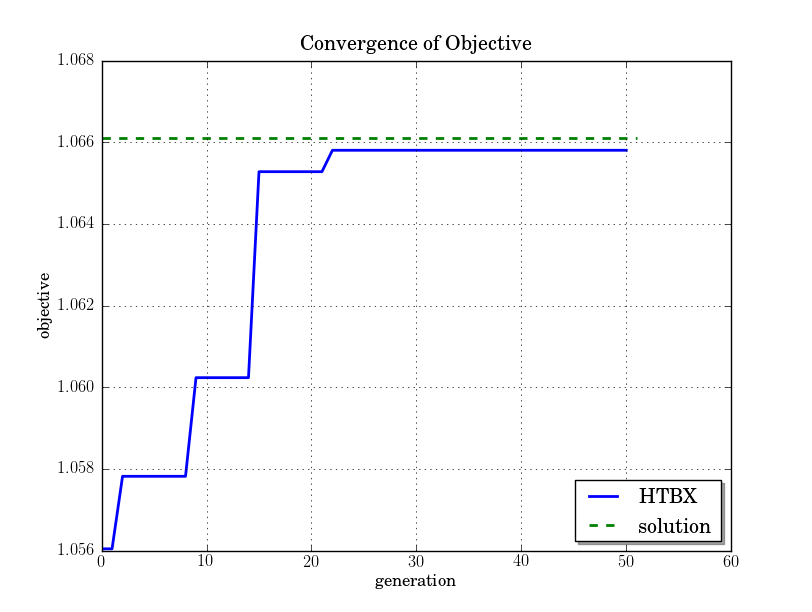
\includegraphics{slab.png}


\chapter{Methods}
\label{methods:sec-methods}\label{methods::doc}\label{methods:methods}
To be completed.


\chapter{API Reference}
\label{api_reference:api-reference}\label{api_reference:sec-reference}\label{api_reference::doc}

\section{Introduction}
\label{api_reference:introduction}
This section provides a reference for all functions
defined in the \code{pypgapack} module that are \emph{extensions} of the basic
PGAPack API.  All PGAPack functions are contained in the
\code{pypgapack.PGA} class.  The PGAPack library is typically
used as follows:

\begin{Verbatim}[commandchars=\\\{\}]
\PYG{k+kt}{double} \PYG{n}{evaluate}\PYG{p}{(}\PYG{n}{PGAContext} \PYG{o}{*}\PYG{n}{ctx}\PYG{p}{,} \PYG{k+kt}{int} \PYG{n}{p}\PYG{p}{,} \PYG{k+kt}{int} \PYG{n}{pop}\PYG{p}{)}\PYG{p}{;}
\PYG{n}{PGAContext} \PYG{o}{*}\PYG{n}{ctx}\PYG{p}{;}
\PYG{n}{ctx} \PYG{o}{=} \PYG{n}{PGACreate}\PYG{p}{(}\PYG{o}{\&}\PYG{n}{argc}\PYG{p}{,} \PYG{n}{argv}\PYG{p}{,} \PYG{n}{PGA\PYGZus{}DATATYPE\PYGZus{}BINARY}\PYG{p}{,} \PYG{l+m+mi}{100}\PYG{p}{,} \PYG{n}{PGA\PYGZus{}MAXIMIZE}\PYG{p}{)}\PYG{p}{;}
\PYG{n}{PGASetUp}\PYG{p}{(}\PYG{n}{ctx}\PYG{p}{)}\PYG{p}{;}
\PYG{n}{PGARun}\PYG{p}{(}\PYG{n}{ctx}\PYG{p}{,} \PYG{n}{evaluate}\PYG{p}{)}\PYG{p}{;}
\PYG{n}{PGADestroy}\PYG{p}{(}\PYG{n}{ctx}\PYG{p}{)}\PYG{p}{;}
\end{Verbatim}

The \code{ctx} object is created explicitly by the user and then passed as
the first argument to all subsequent function calls, with function
names taking the form \code{PGAxxx}.  For \code{pypgapack}, \code{ctx} is
a \emph{private} member of {\hyperref[api_reference:PGA]{\code{PGA}}} created during construction, and all
{\hyperref[api_reference:PGA]{\code{PGA}}} members drop the \emph{PGA} prefix and the initial
\code{ctx} argument. So, for example,

\begin{Verbatim}[commandchars=\\\{\}]
\PYG{n}{ctx} \PYG{o}{=} \PYG{n}{PGACreate}\PYG{p}{(}\PYG{o}{\&}\PYG{n}{argc}\PYG{p}{,} \PYG{n}{argv}\PYG{p}{,} \PYG{n}{PGA\PYGZus{}DATATYPE\PYGZus{}BINARY}\PYG{p}{,} \PYG{l+m+mi}{100}\PYG{p}{,} \PYG{n}{PGA\PYGZus{}MAXIMIZE}\PYG{p}{)}\PYG{p}{;}
\PYG{n}{PGASetUp}\PYG{p}{(}\PYG{n}{ctx}\PYG{p}{)}\PYG{p}{;}
\end{Verbatim}

in C/C++ becomes

\begin{Verbatim}[commandchars=\\\{\}]
\PYG{n}{obj} \PYG{o}{=} \PYG{n}{pypgapack}\PYG{o}{.}\PYG{n}{PGA}\PYG{p}{(}\PYG{n}{sys}\PYG{o}{.}\PYG{n}{argv}\PYG{p}{,} \PYG{n}{PGA}\PYG{o}{.}\PYG{n}{DATATYPE\PYGZus{}BINARY}\PYG{p}{,} \PYG{l+m+mi}{100}\PYG{p}{,} \PYG{n}{PGA}\PYG{o}{.}\PYG{n}{MAXIMIZE}\PYG{p}{)}
\PYG{n}{obj}\PYG{o}{.}\PYG{n}{SetUp}\PYG{p}{(}\PYG{p}{)}
\end{Verbatim}

in Python. For all functions included in PGAPack, the user is directed to the
pgapack documentation.  What follows is a description of the few new
methods added for \code{pypgapack} that make life in Python a
bit easier.


\section{pypgapack API}
\label{api_reference:pypgapack-api}
The easiest way to see what \code{pypgapack} offers is to
do the following:

\begin{Verbatim}[commandchars=\\\{\}]
\PYG{g+gp}{\textgreater{}\textgreater{}\textgreater{} }\PYG{k+kn}{import} \PYG{n+nn}{pypgapack} \PYG{k+kn}{as} \PYG{n+nn}{pga}
\PYG{g+gp}{\textgreater{}\textgreater{}\textgreater{} }\PYG{n+nb}{dir}\PYG{p}{(}\PYG{n}{pga}\PYG{p}{)}
\PYG{g+go}{['PGA', 'PGA\PYGZus{}swigregister', '\PYGZus{}\PYGZus{}builtins\PYGZus{}\PYGZus{}', '\PYGZus{}\PYGZus{}doc\PYGZus{}\PYGZus{}', '\PYGZus{}\PYGZus{}file\PYGZus{}\PYGZus{}',}
\PYG{g+go}{ '\PYGZus{}\PYGZus{}name\PYGZus{}\PYGZus{}', '\PYGZus{}\PYGZus{}package\PYGZus{}\PYGZus{}', '\PYGZus{}newclass', '\PYGZus{}object', '\PYGZus{}pypgapack',}
\PYG{g+go}{ '\PYGZus{}swig\PYGZus{}getattr', '\PYGZus{}swig\PYGZus{}property', '\PYGZus{}swig\PYGZus{}repr', '\PYGZus{}swig\PYGZus{}setattr',}
\PYG{g+go}{ '\PYGZus{}swig\PYGZus{}setattr\PYGZus{}nondynamic']}
\end{Verbatim}

This command works with any Python module.  Our interest is in the
{\hyperref[api_reference:PGA]{\code{PGA}}} class.  We do the same for this:

\begin{Verbatim}[commandchars=\\\{\}]
\PYG{g+gp}{\textgreater{}\textgreater{}\textgreater{} }\PYG{n+nb}{dir}\PYG{p}{(}\PYG{n}{pga}\PYG{o}{.}\PYG{n}{PGA}\PYG{p}{)}
\PYG{g+go}{['BinaryBuildDatatype', 'BinaryCopyString', 'BinaryCreateString',}
\PYG{g+go}{ 'BinaryDuplicate', 'BinaryHammingDistance', 'BinaryInitString',}
\PYG{g+go}{ 'BinaryMutation', 'BinaryOneptCrossover', 'BinaryPrint',}
\PYG{g+go}{ 'BinaryPrintString', 'BinaryTwoptCrossover', 'BinaryUniformCrossover',...}
\end{Verbatim}

and find a really long list of class members, most of which are
directly from PGAPack.  In the following, we document only those
not included in PGAPack, as use of the PGAPack functionality is
covered above (i.e. drop the \code{ctx} argument and \code{PGA} prefix).
\index{PGA (built-in class)}

\begin{fulllineitems}
\phantomsection\label{api_reference:PGA}\pysigline{\strong{class }\bfcode{PGA}}
PGA wrapper class.
\index{\_\_init\_\_() (PGA method)}

\begin{fulllineitems}
\phantomsection\label{api_reference:PGA.__init__}\pysiglinewithargsret{\bfcode{\_\_init\_\_}}{\emph{argv}, \emph{datatype}, \emph{n}, \emph{direction}}{}
Construct the PGA context.  This essentially wraps the PGACreate
function, so see the PGAPack documentation.
\begin{quote}\begin{description}
\item[{Parameters}] \leavevmode\begin{itemize}
\item {} 
\textbf{argv} -- system argument

\item {} 
\textbf{datatype} -- allele dataype; can be \code{PGA.DATATYPE\_XXX},
where \code{XXX} is \code{BINARY}, \code{INTEGER}, and so on.

\item {} 
\textbf{n} -- size of the unknown, i.e. number of alleles of type
\code{datatype}

\item {} 
\textbf{direction} -- either \code{PGA.MAXIMIZE} or \code{PGA.MINIMIZE}

\end{itemize}

\end{description}\end{quote}

\end{fulllineitems}

\index{GetIntegerChromosome() (PGA method)}

\begin{fulllineitems}
\phantomsection\label{api_reference:PGA.GetIntegerChromosome}\pysiglinewithargsret{\bfcode{GetIntegerChromosome}}{\emph{p}, \emph{pop}}{}
Get direct access to the \emph{p}-th integer chromosome string in
population \emph{pop} .
\begin{quote}\begin{description}
\item[{Parameters}] \leavevmode\begin{itemize}
\item {} 
\textbf{p} -- string index

\item {} 
\textbf{pop} -- population index

\end{itemize}

\item[{Returns}] \leavevmode
string as numpy array of integers

\end{description}\end{quote}

\end{fulllineitems}

\index{GetRealChromosome() (PGA method)}

\begin{fulllineitems}
\phantomsection\label{api_reference:PGA.GetRealChromosome}\pysiglinewithargsret{\bfcode{GetRealChromosome}}{\emph{p}, \emph{pop}}{}
Get direct access to the \emph{p}-th double chromosome string in population \emph{pop}.
\begin{quote}\begin{description}
\item[{Parameters}] \leavevmode\begin{itemize}
\item {} 
\textbf{p} -- string index

\item {} 
\textbf{pop} -- population index

\end{itemize}

\item[{Returns}] \leavevmode
string as numpy array of floats

\end{description}\end{quote}

\end{fulllineitems}

\index{SetInitString() (PGA method)}

\begin{fulllineitems}
\phantomsection\label{api_reference:PGA.SetInitString}\pysiglinewithargsret{\bfcode{SetInitString}}{\emph{f}}{}
Set a function for initializing strings.  The function \code{f} provided
\textbf{must} have the signature \code{f(p, pop)}, but should almost certainly
be an inerited class member with the signature \code{f(self, p, pop)}.
See PGAPack documentation for more about user functions.
\begin{quote}\begin{description}
\item[{Parameters}] \leavevmode
\textbf{f} -- Python function

\end{description}\end{quote}


\strong{See Also:}


{\hyperref[examples:sec-initstringexamples]{\emph{Example 4: User-defined String Initialization}}} for an example on string initialization.



\end{fulllineitems}

\index{SetCrossover() (PGA method)}

\begin{fulllineitems}
\phantomsection\label{api_reference:PGA.SetCrossover}\pysiglinewithargsret{\bfcode{SetCrossover}}{\emph{f}}{}
Set a function for the crossover operation.  The function \code{f} provided
\textbf{must} have the signature \code{f(a,b,c,d,e,f)}, but should almost
certainly be an inerited class member with the signature
\code{f(self,a,b,c,d,e,f)}.
See PGAPack documentation for more about user functions.
\begin{quote}\begin{description}
\item[{Parameters}] \leavevmode
\textbf{f} -- Python function

\end{description}\end{quote}


\strong{See Also:}


{\hyperref[examples:sec-crossoverexamples]{\emph{Example 5: User-defined Crossover Operator}}} for an example on setting the crossover
operator.



\end{fulllineitems}

\index{SetMutation() (PGA method)}

\begin{fulllineitems}
\phantomsection\label{api_reference:PGA.SetMutation}\pysiglinewithargsret{\bfcode{SetMutation}}{\emph{f}}{}
Set a function for the mutation operator.  The function \code{f} provided
\textbf{must} have the signature \code{f(p, pop, prob)}, but should almost
certainly be an inerited class member with the signature
\code{f(self, p, pop, prob)}.
See PGAPack documentation for more about user functions.
\begin{quote}\begin{description}
\item[{Parameters}] \leavevmode
\textbf{f} -- Python function

\end{description}\end{quote}


\strong{See Also:}


{\hyperref[examples:sec-mutationexamples]{\emph{Example 6: User-defined Mutation Operator}}} for an example on setting the mutation
operator.



\end{fulllineitems}

\index{SetEndOfGen() (PGA method)}

\begin{fulllineitems}
\phantomsection\label{api_reference:PGA.SetEndOfGen}\pysiglinewithargsret{\bfcode{SetEndOfGen}}{\emph{f}}{}
Set a function for an operator to be performed at the end of each
generation.  The function \code{f} provided
\textbf{must} have the signature \code{f(pop)}, but should almost certainly
be an inerited class member with the signature \code{f(self, pop)}.
Such an operator can be used to implement hill-climbing heuristics.
See PGAPack documentation for more about user functions.
\begin{quote}\begin{description}
\item[{Parameters}] \leavevmode
\textbf{f} -- Python function

\end{description}\end{quote}


\strong{See Also:}


{\hyperref[examples:sec-endofgenexamples]{\emph{Example 7: User-defined End of Generation Operator}}} for an example on setting the an end of
generation operator.



\end{fulllineitems}


\end{fulllineitems}



\chapter{License}
\label{license:sec-license}\label{license::doc}\label{license:license}
\code{pypgapack} itself is licensed under the MIT license, as follows:

\begin{Verbatim}[commandchars=\\\{\}]
Copyright (c) 2011 Jeremy Roberts

Permission is hereby granted, free of charge, to any 
person obtaining a copy of this software and associated 
documentation files (the "Software"), to deal in the 
Software without restriction, including without limitation 
the rights to use, copy, modify, merge, publish, distribute, 
sublicense, and/or sell copies of the Software, and to 
permit persons to whom the Software is furnished to do so, 
subject to the following conditions:

The above copyright notice and this permission notice shall 
be included in all copies or substantial portions of the Software.

THE SOFTWARE IS PROVIDED "AS IS", WITHOUT WARRANTY OF ANY KIND, 
EXPRESS OR IMPLIED, INCLUDING BUT NOT LIMITED TO THE WARRANTIES 
OF MERCHANTABILITY, FITNESS FOR A PARTICULAR PURPOSE AND 
NONINFRINGEMENT. IN NO EVENT SHALL THE AUTHORS OR COPYRIGHT 
HOLDERS BE LIABLE FOR ANY CLAIM, DAMAGES OR OTHER LIABILITY, 
WHETHER IN AN ACTION OF CONTRACT, TORT OR OTHERWISE, ARISING 
FROM, OUT OF OR IN CONNECTION WITH THE SOFTWARE OR THE USE OR 
OTHER DEALINGS IN THE SOFTWARE.
\end{Verbatim}

PGAPack is under its own U-Chicago license that explicitly allows derivatives and redistribution:

\begin{Verbatim}[commandchars=\\\{\}]
COPYRIGHT

The following is a notice of limited availability of the code, and disclaimer
which must be included in the prologue of the code and in all source listings
of the code.

(C) COPYRIGHT 2008 University of Chicago

Permission is hereby granted to use, reproduce, prepare derivative works, and
to redistribute to others. This software was authored by:

D. Levine
Mathematics and Computer Science Division 
Argonne National Laboratory Group

with programming assistance of participants in Argonne National 
Laboratory's SERS program.

GOVERNMENT LICENSE

Portions of this material resulted from work developed under a
U.S. Government Contract and are subject to the following license: the
Government is granted for itself and others acting on its behalf a paid-up,
nonexclusive, irrevocable worldwide license in this computer software to
reproduce, prepare derivative works, and perform publicly and display
publicly.

DISCLAIMER

This computer code material was prepared, in part, as an account of work
sponsored by an agency of the United States Government. Neither the United
States, nor the University of Chicago, nor any of their employees, makes any
warranty express or implied, or assumes any legal liability or responsibility
for the accuracy, completeness, or usefulness of any information, apparatus,
product, or process disclosed, or represents that its use would not infringe
privately owned rights.
\end{Verbatim}


\chapter{Indices and tables}
\label{index:indices-and-tables}\begin{itemize}
\item {} 
\emph{genindex}

\item {} 
\emph{modindex}

\item {} 
\emph{search}

\end{itemize}



\renewcommand{\indexname}{Index}
\printindex
\end{document}
